% !TEX program = lualatex
% Online appendix to the working paper. Built from the thesis text: everything
% here was cut from paper.tex. Tables and figures come from Tables_and_Figures/.
\documentclass[12pt]{article}
% Shared preamble for paper.tex and online_appendix.tex
% Standard economics working-paper layout: 12pt, 1-inch margins, 1.5 spacing,
% author-year citations. Compile with LuaLaTeX.

\usepackage[margin=1in]{geometry}
\usepackage{setspace}
\onehalfspacing
\usepackage{amsmath, amssymb}
\usepackage{graphicx}
\graphicspath{{Tables_and_Figures/figures/}{static_figures/}}
\usepackage{booktabs, tabularx, threeparttable, array, makecell, longtable}
\usepackage{ragged2e}
\usepackage{placeins}
\usepackage{xcolor}
\usepackage[bottom]{footmisc}
\usepackage[font=small, labelfont=bf]{caption}
\usepackage{enumitem}
\setlist{itemsep=2pt, topsep=4pt}

% Author-year citations, as in most economics working papers
\usepackage[backend=biber, style=authoryear, natbib=true, maxcitenames=2,
  uniquename=false, uniquelist=false, giveninits=true, dashed=false]{biblatex}
\addbibresource{articles.bib}
% Undated web sources show "n.d." instead of the year they were accessed
\DeclareLabeldate{\field{date}\field{year}\field{eventdate}\field{origdate}\literal{nodate}}
% Let long URLs in the references break across lines
\usepackage{xurl}
\setcounter{biburllcpenalty}{7000}
\setcounter{biburlucpenalty}{8000}
\setcounter{biburlnumpenalty}{9000}

% Web links are blue and clickable; internal references and citations stay
% black but are still clickable. URLs use the same font as the text.
\usepackage[colorlinks=true, urlcolor=blue, filecolor=blue, linkcolor=black, citecolor=black]{hyperref}
\urlstyle{same}
\newcommand{\appendixurl}{https://github.com/calvinpan1/thesis_india_diaspora_engagement_policies/blob/main/online_appendix.pdf}
\newcommand{\repourl}{https://github.com/calvinpan1/thesis_india_diaspora_engagement_policies}

% Column types and helpers used by the generated tables
\newcolumntype{L}[1]{>{\RaggedRight\arraybackslash}p{#1}}
\newcolumntype{Y}{>{\RaggedRight\arraybackslash}X}
\newcolumntype{Z}{>{\Centering\arraybackslash}X}
\newcolumntype{C}[1]{>{\Centering\arraybackslash}p{#1}}
\renewcommand{\arraystretch}{1.2}
\setlength{\emergencystretch}{2em}
\setlength{\LTcapwidth}{\textwidth}
\newcommand{\fulltablenote}[2]{%
  \multicolumn{#1}{@{}>{\RaggedRight\arraybackslash}p{\dimexpr\linewidth-2\tabcolsep\relax}@{}}{\footnotesize #2}\\%
}

% Tables and figures read single-spaced
\AtBeginEnvironment{table}{\singlespacing}
\AtBeginEnvironment{figure}{\singlespacing}
\AtBeginEnvironment{longtable}{\singlespacing}

% Generated by make_crossrefs.py -- do not edit by hand.
% \oaref{label}: number of a section, table, or figure in the online appendix.
% \pref{label}:  number of a section, table, or figure in the paper.
\newcommand{\oaref}[1]{\ifcsname oaref@#1\endcsname\csname oaref@#1\endcsname\else\textbf{??}\fi}
\newcommand{\pref}[1]{\ifcsname pref@#1\endcsname\csname pref@#1\endcsname\else\textbf{??}\fi}
\expandafter\def\csname oaref@FDI threats\endcsname{4.1.2}
\expandafter\def\csname oaref@fig:Non-Econ vs Econ\endcsname{A15}
\expandafter\def\csname oaref@fig:admin_unit_creation_date\endcsname{A19}
\expandafter\def\csname oaref@fig:all companies by sector\endcsname{A22}
\expandafter\def\csname oaref@fig:bengali speakers\endcsname{A5}
\expandafter\def\csname oaref@fig:commercialcount\endcsname{A11}
\expandafter\def\csname oaref@fig:dravidian_languages\endcsname{A2}
\expandafter\def\csname oaref@fig:econ DEP types over time\endcsname{A20}
\expandafter\def\csname oaref@fig:econ DEPs by state\endcsname{A17}
\expandafter\def\csname oaref@fig:fditop50_noindialine\endcsname{A7}
\expandafter\def\csname oaref@fig:fdivalue\endcsname{A8}
\expandafter\def\csname oaref@fig:ictcount\endcsname{A10}
\expandafter\def\csname oaref@fig:indo_aryan_key\endcsname{A1}
\expandafter\def\csname oaref@fig:info_timing\endcsname{A21}
\expandafter\def\csname oaref@fig:jaccard\endcsname{A18}
\expandafter\def\csname oaref@fig:jobs\endcsname{A9}
\expandafter\def\csname oaref@fig:nepali speakers\endcsname{A6}
\expandafter\def\csname oaref@fig:non-econ DEPs by state\endcsname{A16}
\expandafter\def\csname oaref@fig:punjabisovertime\endcsname{A3}
\expandafter\def\csname oaref@fig:sample 3\endcsname{A14}
\expandafter\def\csname oaref@fig:sample1\endcsname{A13}
\expandafter\def\csname oaref@fig:sample1 gujarati diaspora\endcsname{A12}
\expandafter\def\csname oaref@fig:tamil speakers\endcsname{A4}
\expandafter\def\csname oaref@sec:oa_deps\endcsname{5}
\expandafter\def\csname oaref@sec:oa_discussion\endcsname{8}
\expandafter\def\csname oaref@sec:oa_identification\endcsname{6}
\expandafter\def\csname oaref@sec:oa_measurement\endcsname{4}
\expandafter\def\csname oaref@sec:oa_replication\endcsname{1}
\expandafter\def\csname oaref@sec:oa_results\endcsname{7}
\expandafter\def\csname oaref@sec:oa_roadmap\endcsname{2}
\expandafter\def\csname oaref@sec:oa_states\endcsname{3}
\expandafter\def\csname oaref@sec:oa_techhubs\endcsname{9}
\expandafter\def\csname oaref@ss: bundled, rare policies\endcsname{6.4}
\expandafter\def\csname oaref@ss: model mechanics\endcsname{6.5}
\expandafter\def\csname oaref@ss: sector\endcsname{7.1}
\expandafter\def\csname oaref@ss:activity\endcsname{7.2}
\expandafter\def\csname oaref@ss:are there deps\endcsname{3.2}
\expandafter\def\csname oaref@ss:comp size\endcsname{7.3}
\expandafter\def\csname oaref@ss:diaspora description\endcsname{4.2.4}
\expandafter\def\csname oaref@ss:diaspora languages, state selection\endcsname{3.1}
\expandafter\def\csname oaref@ss:diaspora_measurement_strategy\endcsname{4.2.1}
\expandafter\def\csname oaref@ss:endogeneity\endcsname{6.8}
\expandafter\def\csname oaref@ss:expectations\endcsname{6.9}
\expandafter\def\csname oaref@ss:ict\endcsname{7.4}
\expandafter\def\csname oaref@ss:logical threats\endcsname{6.6}
\expandafter\def\csname oaref@ss:operationalizing DEPs\endcsname{5.2}
\expandafter\def\csname oaref@ss:operationalizing FDI\endcsname{4.1}
\expandafter\def\csname oaref@ss:operationalizing diasporas\endcsname{4.2}
\expandafter\def\csname oaref@ss:reliability\endcsname{4.2.3}
\expandafter\def\csname oaref@ss:samples\endcsname{4.2.2}
\expandafter\def\csname oaref@ss:source_country_roadmap\endcsname{2.1}
\expandafter\def\csname oaref@ss:specification\endcsname{6.2}
\expandafter\def\csname oaref@ss:spillovers\endcsname{6.7}
\expandafter\def\csname oaref@ss:why the us?\endcsname{2.2}
\expandafter\def\csname oaref@ss:why_ppml\endcsname{6.1}
\expandafter\def\csname oaref@subsection:DEPs descriptives\endcsname{5.2.1}
\expandafter\def\csname oaref@subsection:FDI descriptives\endcsname{4.1.3}
\expandafter\def\csname oaref@subsection:no operationalizing DDI\endcsname{4.1.1}
\expandafter\def\csname oaref@tab:appendix_singlepolicy\endcsname{A25}
\expandafter\def\csname oaref@tab:dep_turnon_events\endcsname{A7}
\expandafter\def\csname oaref@tab:final_activity_appendix_singlepolicy\endcsname{A12}
\expandafter\def\csname oaref@tab:final_activity_table2_h1\endcsname{A10}
\expandafter\def\csname oaref@tab:final_activity_table4_h3\endcsname{A11}
\expandafter\def\csname oaref@tab:final_cluster_appendix_singlepolicy\endcsname{A9}
\expandafter\def\csname oaref@tab:final_cluster_table4_h3\endcsname{A8}
\expandafter\def\csname oaref@tab:final_company_size_h0\endcsname{A13}
\expandafter\def\csname oaref@tab:final_company_size_table1_baseline\endcsname{A14}
\expandafter\def\csname oaref@tab:final_company_size_table3_h2\endcsname{A15}
\expandafter\def\csname oaref@tab:final_ict_company_size_appendix_singlepolicy\endcsname{A22}
\expandafter\def\csname oaref@tab:final_ict_company_size_table2_h1\endcsname{A20}
\expandafter\def\csname oaref@tab:final_ict_company_size_table4_h3\endcsname{A21}
\expandafter\def\csname oaref@tab:final_ict_company_size_techhubs_table2_h1\endcsname{A23}
\expandafter\def\csname oaref@tab:final_ict_company_size_techhubs_table4_h3\endcsname{A24}
\expandafter\def\csname oaref@tab:final_ict_generations_education_appendix_singlepolicy\endcsname{A17}
\expandafter\def\csname oaref@tab:final_ict_generations_education_table4_h3\endcsname{A16}
\expandafter\def\csname oaref@tab:final_ict_worker_appendix_singlepolicy\endcsname{A19}
\expandafter\def\csname oaref@tab:final_ict_worker_table2_h1\endcsname{A18}
\expandafter\def\csname oaref@tab:jaccard_top10\endcsname{A6}
\expandafter\def\csname oaref@tab:language_fdi_a1\endcsname{A2}
\expandafter\def\csname oaref@tab:language_fdi_a2\endcsname{A3}
\expandafter\def\csname oaref@tab:language_fdi_a3\endcsname{A4}
\expandafter\def\csname oaref@tab:language_fdi_a4\endcsname{A5}
\expandafter\def\csname oaref@tab:language_fdi_sample\endcsname{A1}
\expandafter\def\csname oaref@tab:single_firm_tech_localities\endcsname{A26}


% Keep each section's tables and figures inside that section
\let\oldsection\section
\renewcommand{\section}{\FloatBarrier\oldsection}
\let\oldsubsection\subsection
\renewcommand{\subsection}{\FloatBarrier\oldsubsection}

% Language tables (Section 3) use these
\newcommand{\apptablefontsize}{\footnotesize}
\newcommand{\apptablespacing}{\setstretch{1}}
\newcommand{\langtableheader}{
\toprule
State
& \makecell[l]{Dominant\\language}
& \makecell[l]{In ACS\\data?}
& \makecell[l]{\% pop.\\L1}
& \makecell[l]{Significant L1 in\\other Indian state?}
& \makecell[l]{Significant L1 in\\other country?}
& \makecell[l]{Avg. US FDI,\\2005--17\\(2023 USD)} \\
\midrule
}

% Appendix floats are numbered A1, A2, ... so they never clash with the paper
\renewcommand{\thetable}{A\arabic{table}}
\renewcommand{\thefigure}{A\arabic{figure}}

\title{Online Appendix to ``Do Subnational Diaspora Engagement Policies Attract FDI? Evidence from India''}
\author{Calvin Pan}
\date{October 2026}

\begin{document}
\maketitle
\tableofcontents
\newpage


\section{Replication Package} \label{sec:oa_replication}

Every data-driven table and figure in the paper and this appendix is rebuilt by one Stata do file, \texttt{0\_master.do} in the \texttt{Syntax} folder, which takes about seven minutes. The package runs in four stages: \texttt{1\_build} reads the IPUMS ACS extract once and keeps everyone born in India or speaking an Indian state language; \texttt{2\_clean} builds the diaspora samples, the FDI extracts, and the DEP panels and merges them; \texttt{3\_tables} writes every table; and \texttt{4\_figures} writes every figure. Each output file starts with the stage and script that made it.

Two data sources cannot be redistributed. IPUMS USA microdata must be downloaded by each user; the README lists the exact extract (the 2005--2017 ACS 1-year samples and the variables YEAR, STATEFIP, MET2013, PERWT, AGE, BPL, LANGUAGE, EDUC, and OCC1990). fDi Markets project data and CRSP matches are licensed, so the package instead ships aggregated extracts built from them: project counts by US metro, Indian state, and year; state-year totals of projects, capital, and jobs; projects by sector; and the investor-name shares in Figure~\pref{fig:indian_names} of the paper. The DEP and DEP budget data are original to this project and are included in full.

Both \texttt{paper.tex} and \texttt{online\_appendix.tex} compile with LuaLaTeX from the root of the package.


\section{Case Selection: A Roadmap for Studying Subnational DEPs} \label{sec:oa_roadmap}

This section lays out the five filters summarized in Section~\pref{sec:setting} of the paper and walks through which countries pass them.

It is incredibly difficult to do a multi-country study on subnational DEPs. Even with sending-country FE, recipient-country FE, and a host of other fixed effects, any such study would require controlling for time-varying differences between the countries that may affect both DEPs and DDI. Possible threats include adoption of other policies, spikes in national or local corruption, tech booms in one sector in one country but not the other that disproportionately affect high-diaspora-population countries. As such, any empirical study must begin with the selection of a single DDI source country and a single DDI recipient country. 

        \subsection{A Roadmap for Selecting Source Countries} \label{ss:source_country_roadmap}
Any DDI source country/subnational diaspora home country we select must pass five essential conditions. 

    First, the country must 1a) have subnational diasporas that conceptualize themselves as separate diasporas. Our whole theory of subnational DDI relies on diaspora individuals from certain regions behaving differently than those from other regions, which then amplifies the mechanisms for DDI we discussed. Additionally, the country must 1b) be multilingual. As detailed later, this is primarily a measurement constraint. Though some countries collect census data on individuals' birthplace, this is flawed as a construct because it excludes second+ generation  diaspora and remigrants (e.g. German-speaking individuals born in Poland who may think of themselves as German will be recorded as Polish). Primary language is thus a more reliable measure of diaspora, though there are issues with this still that will be addressed later. These first filters wash out countries like Mexico that may have subnational DEPs but unfortunately are unmeasurable with our empirical strategy.

    Second, the country must have administrative units that map closely to languages. Put differently, these administrative units must not be under-inclusive of the area where the language is spoken. This can be because the language area is divided into two or more administrative units within the country (e.g. people from Catalonia, Valencia, and the Balearics all being recorded as just Catalan speakers). These situations pose a problem because diaspora may feel attached to one unit, both, or neither; and because two+ separate subnational DEPs may be trying to attract FDI from the individual at once. This problem can also emerge when the language area extends outside of the country. This poses a problem because, for example, Swiss French, Italian, and German subnational diaspora members would just appear as French, Italian, and German speakers in data. This problem can be bypassed if the language diaspora in a country is  largely from a single subnational unit. For example, even though French speakers exist in both France and Switzerland and Swiss French are administered by 7 Swiss cantons, the French-speaking diaspora in South Korea could be 95\% from Switzerland and 90\% from the canton of Geneva. Note that this is conditional on the 10\%  of non-Genevans and 90\% of Genevans sharing similar enough characteristics that the 10\% do not disproportionately dominate DDI to Geneva.

    The countries with regions that pass these first two filters are:
\begin{itemize}
    \item Russia's 20+ minority-language republics,
    \item Belgium (assuming Flemish and Walloon are coded separately in available data from French and German),
    \item Spain: Galicia \footnote{Catalan and Basque fail due to multi-provincial language areas, but Galician could pass conditional on Portuguese Galician diaspora not dominating Spanish Galician.}
    \item China: Hunan (Xiang), Jiangxi (Gan), possibly Guangxi (Ping), southern Anhui (Hui) \footnote{Cantonese fails due to Hong Kong, Guangdong, and Guangxi; Wu fails due to Shanghai, Zhejiang, and Jiangsu. Hakka and Min/Fujianese provisionally fail due to large populations in Taiwan, Southeast Asia, and elsewhere that speak it, but if one can demonstrate that Hakka/Min diasporas from Taiwan/SEA still have a positive effect on investment to the mainland, this may stand.}
    \item India: for the non-Hindi speaking provinces\footnote{Tamil Nadu runs into issues with Sri Lanka, West Bengal with Bangladesh, and Punjab with Pakistan, but as demonstrated later those can be ignored dependent on sending-country diaspora percentages.} 
    \item Ethiopia
    \item Indonesia: Bengkulu, Aceh, Bali, various other provinces in Borneo, Sulawesi, Nusa Tenggara and Papua\footnote{Essentially anywhere that does not speak Javanese, Sundanese, Malayan, or any other multi-provincial language predominantly. Note that many of those provinces are multi-lingual, so regency-level DEPs may be a better fit for analysis.}
    \item Phillippines\footnote{Excluding languages that cross either province or regional lines, depending the administrative division that implements the DEP.}
\end{itemize}

    Third, some of those subnational units of interest must actually have DEPs, so that we can compare them to control units without DEPs. From the list, the following localities have subnational DEPs:
    \begin{itemize}
        \item Russia: Tartarstan, Bashkortostan, and other Republics with strong DEPs \citep{albina_external_2010}.
        \item Spain: Galicia, with its Secretaría Xeral da Emigración \citep{noauthor_galiciaaberta_nodate}.
        \item China, with Overseas Chinese Affairs Offices in many provinces until their 2018 centralization and abolishment \citep{guotu_chinas_2013}.
        \item Ethiopia: only for the Somali Regional State \citep{berhanu_ethiopian_2019}.
        \item India: many non-Hindi speaking states have DEPs, such as Kerala's NORKA \citep{rajan_assessment_2012}.
        \item Indonesia: Nusa Tenggara Timur, Papua, and West Sumatra \citep{noauthor_dinas_nodate, noauthor_badan_nodate, noauthor_portal_nodate}.
        \item Phillippines: with the 2020 creation of Overseas Phillippines Workers Desks in local governments \citep{noauthor_dilg_nodate}.
    \end{itemize}

     Fourth, there should be no simultaneous nation-wide turn-on of those subnational DEPs of interest. Examining the effects of a DEP necessitates control units, and if every single unit turns a DEP on or off simultaneously, there are no control units. This excludes the Phillippines' OPW desks. 
     
     Localities that pass those four filters are ones where, assuming language data availability in the sending country, we can connect DEPs to diasporas. 
    
    Our final filter is that the subnational units with DEPs must receive sufficient amounts of the financial flow in question to make substantial, non-noisy inferences. For this paper, we will focus on just FDI as that is our outcome of interest, but this thinking also applies to remittances and other flows. In a widely-cited article, \citet{desbordes_effects_2017} note that FDI values are a poor measure of multinational expansion because they are net, mix together different kinds of transactions, and can miss real investment funded locally, and argue instead for using project counts. In the fixed-effects Poisson models traditionally used in FDI contexts, sparse data can create low power, many zeros, or separation \citep{santos_silva_further_2011}. five projects/province/year from a single sending country provides high enough precision and low enough shielding from single-year shocks. This equates to around 50 projects/year. \footnote{To benchmark how many projects/year may be needed nationally for this FDI, India had an average of 200 FDI projects/year in 2005-2017 from its largest sending country, the US. At this level of national FDI, the six Indian states that received the most FDI received anywhere from 10 to 50 projects/year from the US. Roughly speaking, a country would then need around 100 projects/year to ensure all of its larger subnational units were analyzable, and perhaps around 20 projects if its FDI was concentrated in just its largest units and it only had a couple subnational units. As a compromise between those two, we will be using 50 projects/year as a benchmark.} 
    
    Using \citet{unctad_world_2025} data on FDI counts, we can examine our chosen subnational units with DEPs:
        \begin{itemize}
        \item Russia (350 projects/year before 2022): Tartarstan and Bashkortostan have large enough cities (Kazan, 6th-largest nationally and Ufa, 10th-largest) that could attract enough FDI to warrant study. There are also a number of other republics with subnational diasporas identifiable by language that can serve as control observations.
        \item Spain (535 projects/year): Galicia could reasonably get enough FDI to warrant study. However, there are no other autonomous communities apart from the Basque Country with subnational diasporas identifiable by language to be control observations.
        \item India (773 projects/year): Enough projects to the point where any province is likely investigatable.
        \item China (1,037 projects/year): Enough projects to the point where any province is likely investigatable.
        \item Ethiopia (14 projects/year): Not enough projects to warrant study.
        \item Indonesia (128 projects/year): Nusa Tenggara Timur, Papua, and West Sumatra could possibly get enough FDI to warrant study, but given how peripheral they are to the national economy, this is unlikely.
    \end{itemize}
    
    Overall, it seems like India and China provide the two most promising cases of subnational DEPs' effects on FDI to investigate, though studies of Tartarstan/Bashkortostan and Galicia could also be worthwhile. This paper will focus on India over China for several reasons. First, there are more Indian subnational units that can be investigated. As will later be demonstrated, eight Indian states present real promise. Meanwhile, only two full Chinese provinces (Hunan and Jiangxi) really stand up to confounding, and neither Xiang nor Gan are recorded in most FDI-sending-country census data.\footnote{For example, US Census Data has not included Xiang as a separate language since 2000, and has not included Gan as a language since at least 1980: https://usa.ipums.org/usa-action/variables/LANGUAGE\#codes\_section} Secondly, there is more variation of what DEPs look like in the Indian case. Though \citeauthor{liu_chinas_2016} show that there was real variation in China's subnational DEPs, they also found that Beijing supplied the ideological and institutional framework for many provincial \textit{qiaowu} policies. In contrast, India's policies largely evolved in contestation with the central Indian state \citep{sharma_partisan_2020} and as such demonstrate more heterogeneity in policy design and mechanisms that could be interesting to investigate.

\subsection{Why the US as our FDI sending country?} \label{ss:why the us?}
    The process of finding an appropriate sending country to measure is much easier now that we have a recipient country. We are choosing the US for four reasons:
    1. The US is, by far, the country that sends the most FDI to India. Over the period 2005-2017 for which I have FDI data, the US sent 35\% of all inward FDI projects to India. The next largest was the UK, with 10\% of all inward FDI projects.
    2. The US has incredibly granular data on languages specifically that enable the collection of data on diaspora FDI. After 2000, the American Community Survey and US Census combined offer yearly estimates of 1\% of the population broken down into 524 languages, including 12 languages spoken in the Indian subcontinent. \citep{noauthor_ipums_nodate} Though UK data has 12 Indian languages as well, there is no ACS equivalent, and so data is only available once every 10 years. \citep{service_language_nodate}
    3. The US has the largest population of non-citizen Persons of Indian Origin (PIO) and citizen Non-Resident Indians (NRI) combined (2.1 million NRI + 3.3 PIO = 5.4 million diaspora). The UAE does have a larger NRI population (3.5 million), but has only 14k PIOs. \citet{noauthor_population_nodate}
    4. Past studies have demonstrated that US FDI abroad is positively correlated with the presence of migrants from the host country. \citet{javorcik_migrant_2011}

\section{Indian States, Languages, and DEP Budgets} \label{sec:oa_states}

This section walks through the first three filters for India in detail: which states' languages map cleanly onto US diasporas, and whether Indian states' DEPs are real.

We will walk through the five aforementioned filters for the case of India to understand its DEP context and determine which states to include in our sample.

\subsection{Filter 1 \& 2: Diaspora Languages and State Selection} \label{ss:diaspora languages, state selection}
On the first filters of 1a) if Indian subnational diasporas exist and 1b) if the country is multilingual, India squarely checks both boxes. India has many languages, with Indo-Aryan languages in the north and Dravidian languages in the south. As aforementioned, diaspora members tend to self-divide and identify along those linguistic lines \citep{sahoo_issues_2006, gautam_indian_2013}. 

\begin{figure}
    \centering
    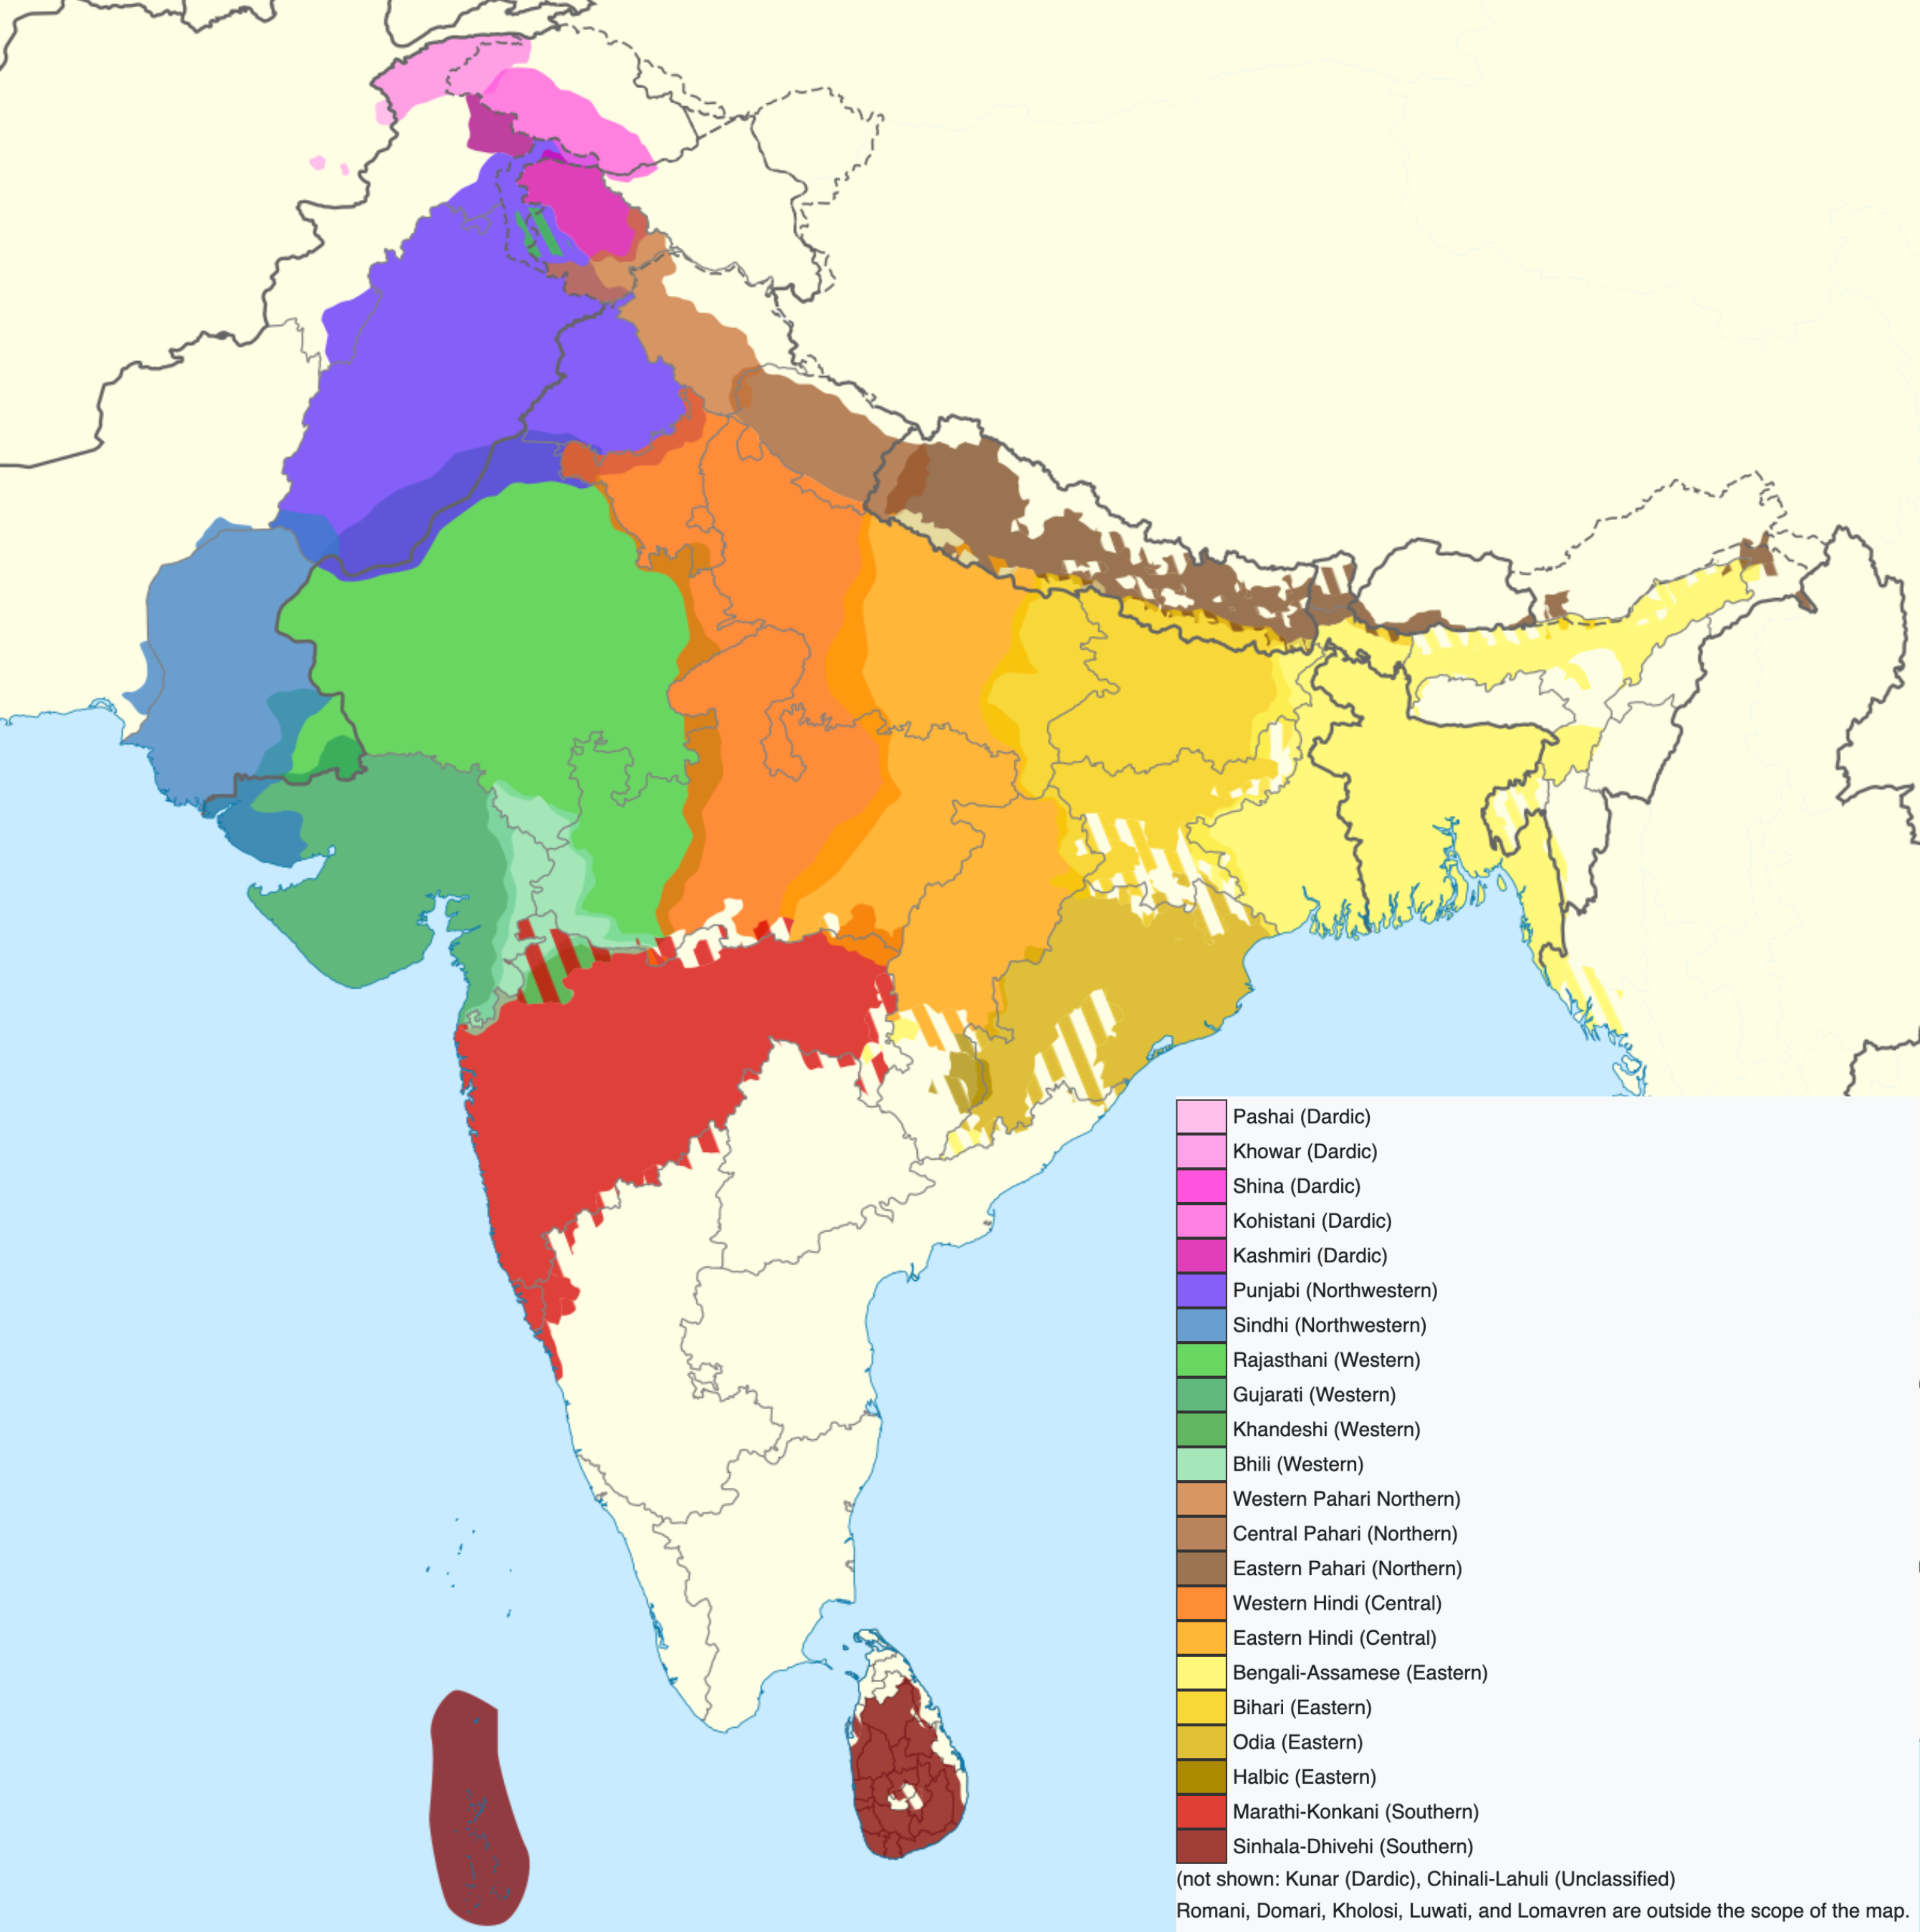
\includegraphics[width=1\linewidth]{indo_aryan_languages.png}
    \caption{Indo-Aryan languages by Indian state. Source: Noahedits, CC BY-SA 4.0 <https://creativecommons.org/licenses/by-sa/4.0>, via Wikimedia Commons \citep{noahedits_english_2020}}
    \label{fig:indo_aryan_key}
\end{figure}
\begin{figure}
    \centering
    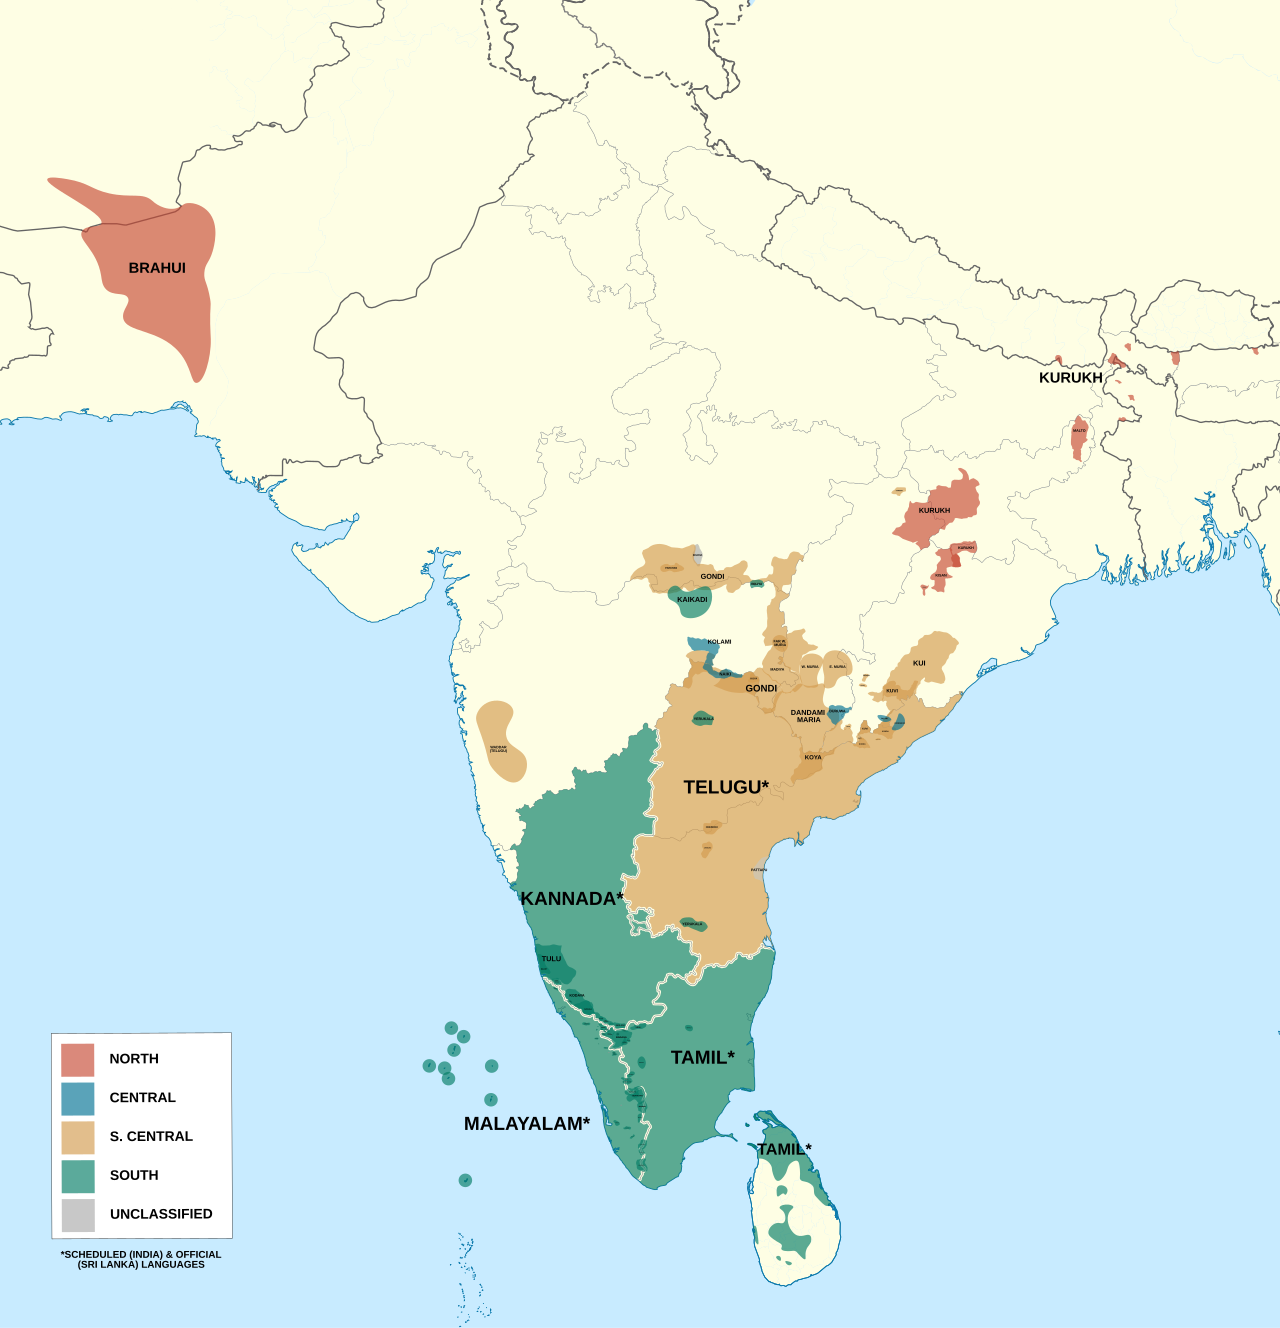
\includegraphics[width=1\linewidth]{dravidian_languages.png}
    \caption{Dravidian languages and Indian states. Source: Own work based on Uwe Dedering, CC BY-SA 3.0 <https://creativecommons.org/licenses/by-sa/3.0>, via Wikimedia Commons \citep{dedering_english_2020}}
    \label{fig:dravidian_languages}
\end{figure}
The second filter, how closely administrative units map to languages, is more problematic: though some languages are mapped to only one state, there are still many exceptions. I decided whether or not to include a state based on four criteria:
\begin{enumerate}
    \item State has one single dominant language 
    \item State’s dominant language is not significantly spoken in any other Indian state
    \item State’s dominant language is not significantly spoken in another country
    \item State has ACS data
\end{enumerate}
A full table of all 28 Indian states and 8 union territories and their ratings on each criterion is included in Section~\ref{sec:oa_states}. In particular, criterion 2 and 3 deserve more detailed discussion.  
    One edge case in criterion 2 was Andhra Pradesh. In 2014, the inland parts of Andhra were split to form Telangana. Both states are still Telugu-language-dominant, and diaspora from both states interact as one single community. This makes identification impossible. As such, Andhra Pradesh will be included in our sample up to the year 2013, and thereafter both Andhra and Telangana will be dropped.
    There were four states that had problems with criterion 3: their language communities crossed state lines. Whether to include those states can be decided based on what percentage of their diasporas in the US is from India vs. the other country. The measures below were constructed using ACS data. 
    
Punjab, our first case, shares the Punjabi language with the Pakistani state of Punjab. Yet, Indian Punjabis are routinely around 10x more numerous in the US than Pakistani Punjabis. As such, Punjabis can be safely kept in the sample as a population.
\begin{figure}
    \centering
    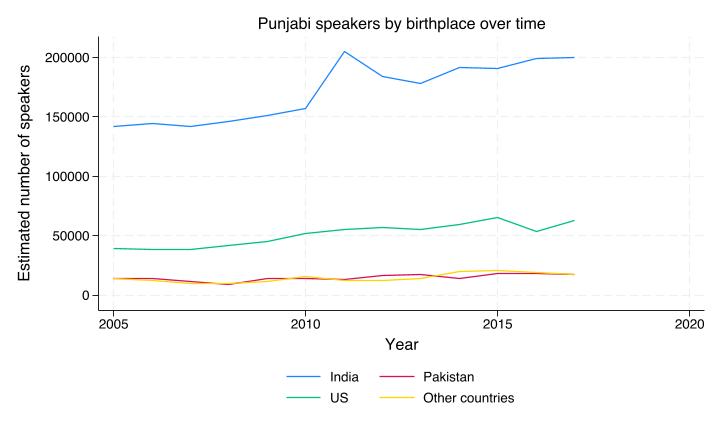
\includegraphics[width=1\linewidth]{4_2_figA3_punjabi_birthplace.png}
    \caption{Punjabi speakers in the US by birthplace. Created by author using ACS data.}
    \label{fig:punjabisovertime}
\end{figure}
Tamil Nadu, our second case, shares the Tamil language with Sri Lanka. Yet, Tamil speakers in the US are almost entirely India-born. As such, Tamils can be safely kept in the sample as a population.
\begin{figure}
    \centering
    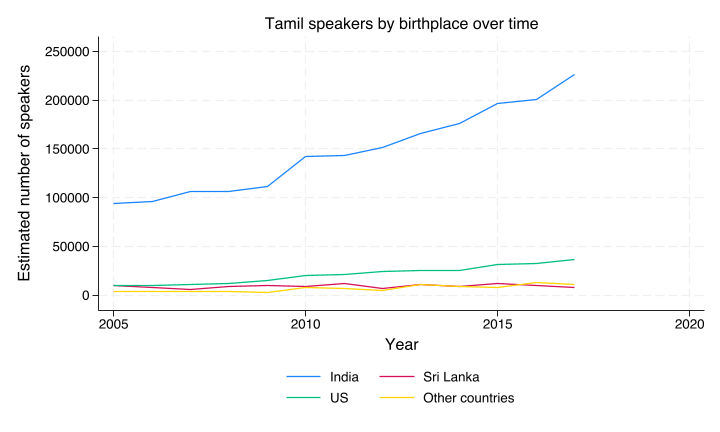
\includegraphics[width=1\linewidth]{4_2_figA4_tamil_birthplace.png}
    \caption{Tamil speakers in the US by birthplace. Created by author using ACS data.}
    \label{fig:tamil speakers}
\end{figure}
West Bengal, our third case, shares the Bengali language with Bangladesh. Contrary to our first couple cases, Bengalis of Indian origin are dwarfed in the US by Bengalis of Bangladeshi origin (who are roughly 3x larger in population). However, they are still a large population (\~90k), and our empirics would increase in confirmatory power if they included an 8th additional state, making the inclusion of West Bengal still worthwhile. If we attempted to include West Bengal by including all Bengali immigrants born in India and also second-generation immigrants marked as born in the US, then most of this second-generation population will likely be those who feel more attachment to Bangladesh rather than West Bengal. Therefore, the only way to include Bengalis is to create a separate sample of all states that only includes first-generation immigrants (i.e. those that are marked as being born in India). We will also exclude West Bengal and Bengali speakers from our larger sample of all-generation all workers.
   \begin{figure}
       \centering
       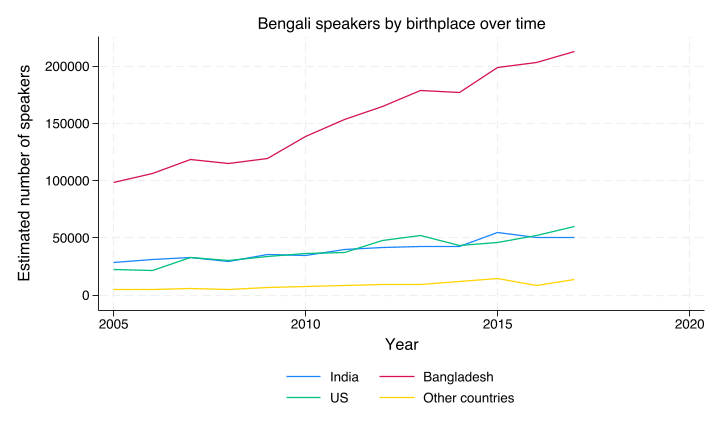
\includegraphics[width=1\linewidth]{4_2_figA5_bengali_birthplace.png}
       \caption{Bengali speakers in the US by birthplace. Created by author using ACS data.}
       \label{fig:bengali speakers}
   \end{figure}
Sikkim, our last case, has a much worse case for inclusion than West Bengal. It shares the Nepali language with Nepal and parts of Bhutan. Yet, there are almost zero Nepali speakers in the US who were born in India. Unlike the Bengal case, the incredibly small population of Indian-born Nepali speakers in the US means that there is no case for their inclusion in either sample.
\begin{figure}
    \centering
    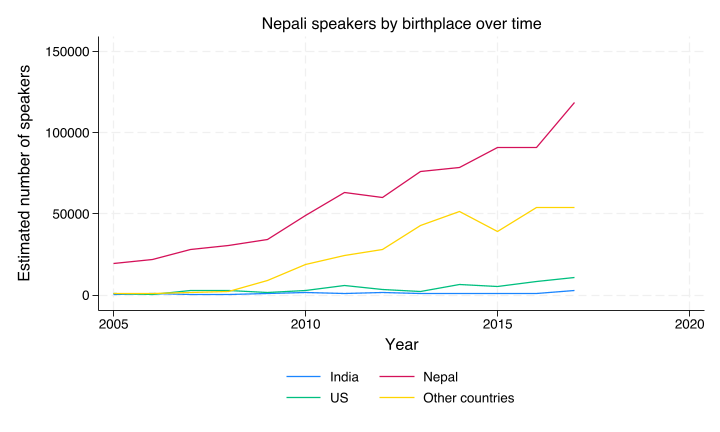
\includegraphics[width=1\linewidth]{4_2_figA6_nepali_birthplace.png}
    \caption{Nepali speakers in the US by birthplace. Created by author using ACS data.}
    \label{fig:nepali speakers}
\end{figure}

After the discussion of criterion 2 and 3, we are left with a sample of 8 states: Tamil Nadu, Kerala, Karnataka, Maharashtra, Andhra Pradesh (before 2014), Gujarat, Punjab, and West Bengal (included in first-gen-only sample, excluded from all-generation sample). This sample includes 5 South Indian states and 3 non-South Indian states, meaning that though it skews relatively to the south of the country, results can be generalized for the rest of India.

\subsection{Filter 3: Do Indian states have real DEPs?}\label{ss:are there deps}
    Before spending a long time coding DEPs, it is wise to qualitatively examine whether DEPs in India are just names in newspaper announcements or governmental websites, or whether they truly exist and do real work. 
   DEPs have also become essential in the minds of many state government decision makers. In Kerala, NORKA has been a top level department since 1996, and has been given its own section almost every year since 2001 in the Kerala Chief Minister's annual budget speeches. In 2016, Chief Minister Oommen Chandy viewed diaspora engagement as an important enough priority that when PM Narendra Modi wanted to merge the national Ministry of Overseas Indian Affairs with the Ministry of External Affairs, he publicly denounced the move as an "insult to the whole NRI community" and met with Modi over it \citep{ttn_team_kerala_2016}. In Punjab, diaspora engagement has also been mentioned in budget speeches since 2017. 
   We know from those budget speeches and state budgets themselves that policy-makers put their money where their mouths were. From 2005 to 2017, Kerala multiplied its DEP budget 43 times, from 1,881 lakhs (2023 INR) to 82,050 lakhs (2023 INR), equivalent to \$88 million in 2026 USD.\footnote{Budgets derive from Kerala budget speeches, 2005-2017, under \citet{noauthor_kerala_nodate}. All new items under any header related to NORKA or NRIs were counted as an increase on the previous budget. Yearly fixed-cost spending on staff, administration, and other general expenses were assumed to be the same if not explicitly mentioned.} Punjab multiplied its budget 220 times, from 158 lakhs to 34,952 lakhs (\$38 million, 2026 USD) \footnote{Data taken from \citet{noauthor_department_nodate} for 2013 onward and from miscellaneous budget documents available online for before 2013. Accounting for all spending, 2005-2017, under headers that mention NRI, which can be found with a search in Non-Plan Budget Book Volume 2/3s and Plan Budget Books. Both revenue and capital expenditures considered.}. From 2010, when it first created a DEP agency, to 2017, Tamil Nadu multipied its DEP budget from 3,268 lakhs to 17,246 lakhs (\$20 million, 2026 USD)\footnote{All line items taken from the Demand No. 38: Public Department books published between 2010 (the renaming of the Department of Rehabilitation to ``Commissionerate of Rehabilitation and Welfare of Non-Resident Tamils')-2017 by the Tamil Nadu government here \citep{noauthor_budget_nodate}
   }. The only state that we have budget data for\footnote{Gujarat and Karnataka had DEPs during this time, but their available budget data did not mention DEPs specifically. For Gujarat, this was likely because I could only find budget speeches, not granular budgets, so this does not indicate the non-intensiveness of DEPs.} which did not see as large of an increase was Andhra Pradesh, which went from 166 lakhs in 2008 to 253 lakhs in 2014 before its partition. \footnote{Budget documents for Andhra Pradesh are hard to find, but I was able to find Appropriations Accounts documents for AP from the 2008 creation of the Andhra Pradesh NRI Cell to 2014, when Andhra was split. Documents look like this one: \citep{government_of_andhra_pradesh_government_2009}.}

   
   These large investments have allowed DEPs to leave a genuine imprint in the migrant consciousness. A 2023 study conducted for NORKA, India's oldest state-level diaspora engagement agency, found that awareness of some NORKA programs is nearing 30\% of all emigrant households, with 29.7\% being aware of the Non-Resident Keralite ID Card and 26.3\% being aware of certificate attestation programs (for proving certification in trades for working overseas) \citep{rajan_kerala_2023}. Evidence from Facebook also shows that they have also reached a large number of individuals: at the time of writing, NORKA Roots had 113K followers and the Non-Resident Gujaratis' Foundation had 76K followers. This rivals Indian national government ministries like the Ministry of Law and Justice (19k followers, founded in 1949) and Ministry of Consumer Affairs (80k followers, founded in 1946). 
   
    This abundance of qualitative evidence that DEPs are prominent in the minds of lawmakers, receive real investment, and in turn are prominent in the minds of migrants enables this paper to code DEP data with confidence that DEPs are more than just 'paper programs.' This evidence also provides a foundation upon which the correlations derived from ensuing quantitative analysis can be plausibly causal.
    
    An important additional learning from those budget speeches is that that policymakers across states have the same primary goal of investment, but very different secondary goals in mind for their DEPs. Policymakers across all states appear to believe that the primary goal of DEPs is to promote NRI investment in the state: budget speeches across Kerala and Punjab reference most frequently ideas like helping "NRIs [who] want to repay their community" \citep{singh_badal_speech_2017}. Where policymakers diverge across states, however, is their secondary goal. In Kerala, budget speech sections on diaspora members are titled "Welfare of Non-Resident Keralites," matching the state's extensive focus on providing welfare for its large overseas population as another key goal of its DEPs \citep{isaac_government_2016}. Meanwhile in Punjab, DEP revenue expenditures are placed under the major head of 2515: Other Rural Development Programs, suggesting that the state views rural development as key secondary goal of DEPs in addition to industrial development \citep{finance_department_punjab_detailed_2013}. States whose DEPs align with the Kerala model of more DEPs in the abroad category will likely have very different outcomes on FDI than those whose DEPs that align with the Punjab model of more economic and specifically economic advantage DEPs.

\subsection{Language classification tables}

\begin{table}[htbp]
\centering
\caption{Languages of Indian states included in sample}
\label{tab:language_fdi_sample}
\begin{threeparttable}
\footnotesize
\setstretch{1}

\begin{tabularx}{\textwidth}{@{}Y Y Z Z Y Y Y@{}}
\toprule
& \makecell[l]{State's\\dominant \\ language}
& \makecell[l]{Is lang. \\ in ACS \\ data?}
& \makecell[l]{\% of\\pop.\\L1}
& \makecell[l]{Is lang.\\signif. L1\\in other\\Indian\\state?}
& \makecell[l]{Is lang.\\signif. L1\\in other\\country?}
& \makecell[l]{Avg. yearly\\US FDI\\to state,\\2005--17\\(2023 USD)} \\
\midrule
Kerala & Malayalam & Y & 97.03\% &Y, but Lakshadweep only (pop 64K, Kerala 36M) & N & \$161M \\
Tamil Nadu & Tamil & Y & 88.37\% & Y, but Puducherry only (pop 1.4M, Tamil Nadu 72M) & N & \$769M \\
Gujarat & Gujarati & Y & 85.97\% & Y, but Daman and Diu (50\% L1, pop 585K) and Dadra and Nagar Haveli (21\% L1, pop 343K) only; Gujarat pop: 66M & N & \$855M \\
Karnataka & Kannada & Y & 66.54\%, no other lang. >10\% L1 & N & N & \$1,519M \\
Maharashtra & Marathi & Y & 68.93\%, 12.9\% Hindi, no other lang. >10\% L1 & N & N & \$1,809M \\
Andhra Pradesh* & Telugu & Y & 83.55\% & Y after 2014 creation of Telangana from Andhra & N & \$1,342M \\
\bottomrule
\end{tabularx}

\begin{tablenotes}[flushleft]
\footnotesize
\item *: Andhra is only included in the sample for the years 2005-2013, as Telangana was split from it in 2014.
\item[Source:] "Language – India, States and Union Territories," Census of India 2011 (Most recent census). Paper 1 of 2018. Office of the Registrar General. pp. 13–14. \url{https://www.censusindia.gov.in/nada/index.php/catalog/42458}
\end{tablenotes}

\end{threeparttable}
\end{table}

\begin{table}[htbp]
\centering
\caption{States with identification problems because other states share their language}
\label{tab:language_fdi_a1}
\begin{threeparttable}
\footnotesize
\setstretch{1}

\begin{tabularx}{\textwidth}{@{}Y Y Z Z Y Y Y@{}}
\toprule
& \makecell[l]{State's\\dominant \\ language}
& \makecell[l]{Is lang. \\ in ACS \\ data?}
& \makecell[l]{\% of\\pop.\\L1}
& \makecell[l]{Is lang.\\signif. L1\\in other\\Indian\\state?}
& \makecell[l]{Is lang.\\signif. L1\\in other\\country?}
& \makecell[l]{Avg. yearly\\US FDI\\to state,\\2005--17\\(2023 USD)} \\
\midrule
% States with identification problems because other states share their language
Telangana & Telugu & Y & 75.5\%\textsuperscript{1} & Y after 2014 creation of Telangana from Andhra & N & \$535M\textsuperscript{2} \\
Himachal Pradesh & Hindi & Y & 85.88\% & Y, Hindi belt & N & \$81M \\
Chandigarh & Hindi & Y & 73.60\% & Y, Hindi belt & N & \$34M \\
Uttarakhand & Hindi & Y & 89.15\% & Y, Hindi belt & N & \$43M \\
Haryana & Hindi & Y & 88.05\% & Y, Hindi belt & N & \$458M \\
NCT of Delhi & Hindi & Y & 84.92\% & Y, Hindi belt & N & \$418M \\
Rajasthan & Hindi & Y & 89.39\% & Y, Hindi belt & N & \$119M \\
Uttar Pradesh & Hindi & Y & 94.08\% & Y, Hindi belt & N & \$339M \\
Bihar & Hindi & Y & 77.25\% & Y, Hindi belt & N & \$14M \\
Jharkhand & Hindi & Y & 61.95\% & Y, Hindi belt & N & \$4M \\
Chhattisgarh & Hindi & Y & 83.62\% & Y, Hindi belt & N & \$141M \\
Madhya Pradesh & Hindi & Y & 88.57\% & Y, Hindi belt & N & \$165M \\
Daman \& Diu & Gujarati \& Hindi & Y & Gujarati 50.83\%, Hindi 36.31\% & Y, Gujarat (pop: 66M, Daman \& Diu pop: 585K) & N & \$3M \\
Dadra \& Nagar Haveli & Gujarati \& Hindi & Y & Gujarati 21.48\%, Hindi 26.16\% & Y, Gujarat (pop: 66M, Dadra \& Nagar Haveli pop: 343K) & N & \$0M \\
Lakshadweep & Malyalam & Y & 84.17\% & Y, Kerala  (pop: 36M, Lakshadweep pop: 64K) & N & \$0M \\
Puducherry & Tamil & Y & 88.22\% & Y, Tamil Nadu  (pop: 72M, Puducherry pop: 1.4M) & Y, Sri Lanka (US pop: ) & \$9M \\
Andaman \& Nicobar Islands & 4 languages (Bengali, Hindi, Tamil, Telugu)  & Y & Bengali 28.49\%, Hindi 19.29\%, Tamil 15.20\%, Telugu 13.24\% & Y, states speaking those 4 langs & Y for Tamil, Sri Lanka & \$0M \\
\bottomrule
\end{tabularx}

\begin{tablenotes}[flushleft]
\footnotesize
\item 1: Telangana's Telugu speaker \% was not directly reported in the 2011 Census as Telangana did not exist yet; statistics are tabulated from mandal/locality-level data of the area that became present-day Telangana, excluding mandals transferred to Andhra Pradesh.
\item 2: This average of FDI to Telangana is from 2015 (the year after its creation in 2014) to 2017.
\item[Source:] "Language – India, States and Union Territories," Census of India 2011 (Most recent census). Paper 1 of 2018. Office of the Registrar General. pp. 13–14. \url{https://www.censusindia.gov.in/nada/index.php/catalog/42458}
\end{tablenotes}

\end{threeparttable}
\end{table}

\begin{table}[htbp]
\centering
\caption{States with identification problems because other countries share their language}
\label{tab:language_fdi_a2}
\begin{threeparttable}
\footnotesize
\setstretch{1}

\begin{tabularx}{\textwidth}{@{}Y Y Z Z Y Y Y@{}}
\toprule
& \makecell[l]{State's\\dominant \\ language}
& \makecell[l]{Is lang. \\ in ACS \\ data?}
& \makecell[l]{\% of\\pop.\\L1}
& \makecell[l]{Is lang.\\signif. L1\\in other\\Indian\\state?}
& \makecell[l]{Is lang.\\signif. L1\\in other\\country?}
& \makecell[l]{Avg. yearly\\US FDI\\to state,\\2005--17\\(2023 USD)} \\
\midrule
% States with identification problems because other countries share their language
West \\ Bengal & Bengali & Y & 86.22\% & Y, Tripura (pop: 4.2M, West Bengal pop: 92.1M) & Y, Bangladesh (US: ) & \$116M \\
Tripura & Bengali & Y & 65.73\% & Y, West Bengal (pop: 91M, Tripura pop: 4.2M) & Y, Bangladesh (US: ) & \$0M \\
Sikkim & Nepali & Y & 62.60\%, 7.96\% Hindi, many smaller langs & N & Y, Nepal (US: ) & \$0M \\
\bottomrule
\end{tabularx}

\end{threeparttable}
\end{table}

\begin{table}[htbp]
\centering
\caption{States with identification problems because their language is not in ACS data}
\label{tab:language_fdi_a3}
\begin{threeparttable}
\footnotesize
\setstretch{1}

\begin{tabularx}{\textwidth}{@{}Y Y Z Z Y Y Y@{}}
\toprule
& \makecell[l]{State's\\dominant \\ language}
& \makecell[l]{Is lang. \\ in ACS \\ data?}
& \makecell[l]{\% of\\pop.\\L1}
& \makecell[l]{Is lang.\\signif. L1\\in other\\Indian\\state?}
& \makecell[l]{Is lang.\\signif. L1\\in other\\country?}
& \makecell[l]{Avg. yearly\\US FDI\\to state,\\2005--17\\(2023 USD)} \\
\midrule
% States with identification problems because their language is not in ACS data
Odisha & Odia & N & 82.70\% & N & N & \$8M \\
Goa & Konkani & N & 66.11\% & N & N & \$17M \\
Jammu \& Kashmir & Kashmiri & N & 53.27\%, 20\% Hindi, 20\% Dogri & N & Y, in Pakistani Kashmir & \$0M \\
Manipur & Manipuri & N & 53.30\% & N & N & \$0M \\
Mizoram & Mizo & N & 73.1\% & N & N & \$0M \\
Meghalaya & Khasi \& Garo & N & Khasi 33.8\%, \& Garo 31.6\% & N & N & \$0M \\
Assam & Assamese & N & 48.38\% & N & N & \$1M \\
\bottomrule
\end{tabularx}

\end{threeparttable}
\end{table}

\begin{table}[htbp]
\centering
\caption{States with identification problems because they have no primary language}
\label{tab:language_fdi_a4}
\begin{threeparttable}
\footnotesize
\setstretch{1}

\begin{tabularx}{\textwidth}{@{}Y Y Z Z Y Y Y@{}}
\toprule
& \makecell[l]{State's\\dominant \\ language}
& \makecell[l]{Is lang. \\ in ACS \\ data?}
& \makecell[l]{\% of\\pop.\\L1}
& \makecell[l]{Is lang.\\signif. L1\\in other\\Indian\\state?}
& \makecell[l]{Is lang.\\signif. L1\\in other\\country?}
& \makecell[l]{Avg. yearly\\US FDI\\to state,\\2005--17\\(2023 USD)} \\
\midrule

% States with identification problems because they have no primary language
Arunachal Pradesh & None (many smaller langs) & N/A & N/A & N/A & N/A & \$0M \\
Nagaland & None (many smaller langs) & N/A & N/A & N/A & N/A & \$1M \\
\bottomrule
\end{tabularx}

\end{threeparttable}
\end{table}

\section{Measurement Framework, FDI, and Diaspora Data} \label{sec:oa_measurement}

    We have now demonstrated that India is the best case for us to test our hypotheses with, and that Indian states have sufficiently cleared our first three filters such that a causal relationship between DEPs and DDI can plausibly exist and be proven. We are now ready to discuss how to measure our hypotheses.

    The fundamental equation of all statistical inference, as laid out by \citet{bueno_de_mesquita_thinking_2021}, is below:
\[Estimate = Estimand + Bias + Noise\]
   This can alternatively be expressed as the following:  \[\bar{Y}_{1T}-\bar{Y}_{0U} = 
    [\bar{Y}_{1T}-\bar{Y}_{0T}] + 
    [\bar{Y}_{0T}-\bar{Y}_{0U}] + Noise
    \]
    However, we run into the fundamental problem of causal inference here. We can never observe the counterfactuals for each treatment group ($\bar{Y}_{0T}$ and $\bar{Y}_{1U}$), so both our estimand and bias terms are un-calculatable. We will talk about how to combat this in our research design section. For now, let us rewrite all of our hypotheses in this format. 
    
    The first step is to define our outcome variable, which is the influence of diaspora on FDI at a certain year. Put a different way, this is \[
\Delta_i(t) \equiv Y_i(d_H,t)-Y_i(d_L,t)
\]
    where $d_H$ indicates high diaspora at time $t$ for the locality, and $d_L$ indicates low diaspora at time $t$ for the locality. 

    We can now use this shorthand to rewrite each hypothesis into $Estimate = Estimand + Bias $ form.
    
\textbf{$H_0$:  As the location-specificity of a diaspora group increases, the positive effect it has on foreign direct investment to that location increases.}
\[
\bar{\Delta}_T(1)-\bar{\Delta}_U(0)
=
\left[\bar{\Delta}_T(1)-\bar{\Delta}_T(0)\right]
+
\left[\bar{\Delta}_T(0)-\bar{\Delta}_U(0)\right]
\]
Where $T$ is being part of a highly location-specific diaspora group (e.g. city or state diaspora), and $U$ is being part of a non-location-specific diaspora group (e.g. national diaspora).

\textbf{$H_1$:  As localities adopt any DEP, the positive effect diasporas have on FDI to that locality increases.}
\[
\bar{\Delta}_T(1)-\bar{\Delta}_U(0)
=
\left[\bar{\Delta}_T(1)-\bar{\Delta}_T(0)\right]
+
\left[\bar{\Delta}_T(0)-\bar{\Delta}_U(0)\right]
\]
Where $T$ is the locality having any DEP, and $U$ is the locality having no DEPs.

\textbf{$H_2$:  As localities' number of DEPs increases, the positive effect diasporas have on FDI to that locality increases.}
\[
\bar{\Delta}_T(1)-\bar{\Delta}_U(0)
=
\left[\bar{\Delta}_T(1)-\bar{\Delta}_T(0)\right]
+
\left[\bar{\Delta}_T(0)-\bar{\Delta}_U(0)\right]
\]
Coding as strict binaries is difficult here because this is about dose response, but this can be interpreted as $T$ being the locality having many DEPs, and $U$ being the locality having few DEPs.

\textbf{$H_3$:  As the economic advantage provided by a DEP increases, its impact on DDI becomes more positive.}
\[
\bar{\Delta}_T(1)-\bar{\Delta}_U(0)
=
\left[\bar{\Delta}_T(1)-\bar{\Delta}_T(0)\right]
+
\left[\bar{\Delta}_T(0)-\bar{\Delta}_U(0)\right]
\]
Where $T$ is the locality having a high economic advantage DEP, and $U$ is the locality having a low economic advantage DEP.

    We need to operationalize four variables to be able to measure these equations. For $H_0$, we will need to operationalize the components of $\Delta_it$, 1) diaspora $d_{H/L}$ and 2) FDI $Y_i$. We will also need to operationalize the treatment, 3) diaspora location specificity $T/U$. For $H_{1-3}$, we will need to operationalize another treatment, 4) diaspora engagement policies $T/U$.  

     We know that in order to have zero bias, we need to have $\left[\bar{\Delta}_T(0)-\bar{\Delta}_U(0)\right]$ equal to zero. For this to be true, though, $
\Delta_i(t) \equiv Y_i(d_H,t)-Y_i(d_L,t)$ must be measured without bias. In other words, the error terms $e_i$ in $d_i​=d_i^∗​+e_i$, $Y_i​=Y_i^∗​+e_i$, and $T_i​=T_i^∗​+e_i$ must be zero. 

    There are two ways in which our measurements may cause the error term $e_i$ to be non-zero. The first way is issues with validity. This occurs when there is distance between the theoretical construct we are trying to capture and the empirical strategy we are using to measure it. To use an example from \citet{yeung_self-reported_2025}, if our theoretical construct is how liberal/conservative someone is, but our empirical strategy is just to ask people if they identify more with the term 'liberal' or 'conservative,' then we may run into issues if people's understandings of those terms are "weakly aligned with the conventional definitions of these terms.'
    
    If this distance between the indicator and the construct exists, there are three validity issues we have to worry about. First, the indicator could capture elements that belong to other constructs; second, the indicator could miss theoretical elements that are central to the construct; or third, the application of our operational rules induces systematic measurement errors.

    The other way our measurements could cause error would be issues with reliability. An unreliable measurement is not systematically biased, but rather is randomly noisy and thus can produce readings that are quite far away from reality. Using the earlier example, even if asking someone if they are 'liberal' or 'conservative' does not produce ideology averages that are systematically more liberal or conservative-skewed than reality, this measure may still be unreliable if both liberals respond they are conservative and conservatives respond they are liberal at concerningly high rates. 

   In this paper, I will prioritize making sure my measures are valid before ensuring they are reliable. Though it would be ideal for both to be true, bias should be dealt with before noise is a concern: bias skews our results; noise simply makes them more underpowered. I will discuss each measurement below in terms of how valid and reliable they are.
   
           
        \subsection{Operationalizing FDI} \label{ss:operationalizing FDI}
    The data I have is for FDI is all greenfield FDI projects to India in the fDiMarkets database. To start off with, fDiMarkets collects the date, source US city, and destination Indian state of every FDI project, which is what we will be using to join the FDI database.
    
    \subsubsection{Why we cannot directly operationalize DDI} \label{subsection:no operationalizing DDI}
    Another variable that fDiMarkets collects is investor names for projects where it is available. It would be tempting at this stage to simply code all investors' names by whether they are of Indian origin, and then filter to those projects with Indian names. Unfortunately, this strategy is flawed at several stages.
    Firstly, name data is not available for a lot of observations: 1,080/3,184 projects into India (34\%) are blank in this category. Dropping all those observations would introduce both an issue of error and of power (what if smaller projects or defense-sector projects are more likely to not have investor names)? Secondly, the idea of coding names as Indian or non-Indian introduces a whole host of issues. Even if we had a way to identify Indian names with 100\% accuracy, we would still run into issues like individuals with Indian names not identifying with the diaspora.
    Thirdly, the way fDiMarkets codes these data is that they are those who were recorded making the announcement of the FDI or interviewed in the news release of the article. However, there may be many more diaspora members behind the scenes that helped facilitate investment or indeed were the final decision makers. But even if this dataset was a perfect measure of 'diaspora decision makers,' the fourth concern is that our theory is not about what percentage of DDI was by 'diaspora decision makers,' but rather what the effect of the overall size of a diaspora on investment is by virtue of attributes that all scale with size: networks, knowledge of home region, home preference. Finally and most fatally, we have no reliable way to code what ``subnational DDI'' is from this data. Indian names do differ by state of origin and by caste, but even the best prediction algorithms only have around a \~80\% accuracy, which is too low for our paper. \citep{dhingra_instate_2023}
    We will thus draw from \citet{leblang_familiarity_2010}'s measure of what DDI instead: we will regress diasporas on FDI and capture this effect as DDI. The research design section will specify more about what our exact regression looks like.
   However, this name data can still provide us directional answers about if our construct of DDI is valid. The investors in the dataset had job titles largely recorded as either President, C-Suite, or heads of Indian divisions of companies. Both large multinationals and smaller firms were included, including startups led by diaspora entrepreneurs. I used a script for processing names by geographic origin to check those  \citep{dhingra_instate_2023}. I found that around half of the FDI investors had Indian names and about 1/3rd of all projects were undertaken by them, which is a robust finding on the idea of DDI and that diaspora members in this dataset do influence investment decisions.

    \subsubsection{Threats to measurement reliability and validity} \label{FDI threats}
        There are several threats to $e_i$ being zero in $Y_i​=Y_i^∗​+e_i$. The first possible threat to validity is the error from the way fDiMarkets generates data. The way fDiMarkets works is that their team scrapes public announcements of FDI projects every day and combines that with various other sources of information: government registries, etc. The end goal is to capture all FDI project flows happening around the world. It is therefore the closest thing available to an exhaustive database of FDI inflows. There could very well be systematic observation error in fDiMarkets' data collection strategy, but this would only be harmful if certain India states were disproportionately less captured by the database. I have seen nothing qualitatively or quantitatively to suggest this is occurring. Additionally, their FAQs say that the database undergoes rigorous quality controls before being included in monthly updates, and fDiMarkets is trusted by researchers around the world.
        The second possible threat to validity could come from the joining process to diaspora data. During the process of joining fDiMarkets to ACS data, I had to convert the city names fDiMarkets saved into MET2013 areas. This was done through an ArcGIS spatial join of the coordinates each fDiMarkets city had in the ArcGIS dataset to MET2013 areas, a method which tried to ensure the minimum amount of loss possible. However, a small number of fDiMarkets cities (around 5) had portions in 2 or more MET2013 areas, and so this process may have placed some projects in the wrong metro area. The error from this is likely negligible, and it is also unlikely to be systematically skewed.
    There are several credible threats to reliability. fDiMarkets' announcement-based system likely misses some amount of unannounced FDI projects. The data also may code projects as belonging to the wrong company, state, or sector. However, those limitations exist with any FDI dataset.
        
            \subsubsection{Descriptives of FDI data} \label{subsection:FDI descriptives}
    Project counts data from the FDI markets data can be seen below. In a confirmation of data fidelity, these data clearly show canonical effect of India's 2005 FDI liberalization in 2006, with a large spike in FDI that year that soon tapers off. 
        \begin{figure}
            \centering
            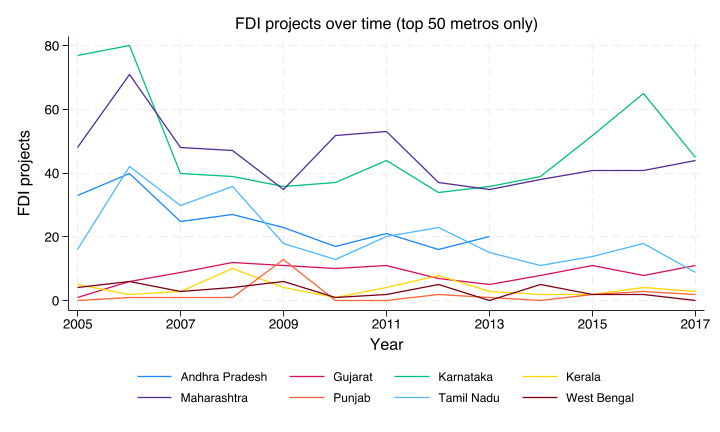
\includegraphics[width=1\linewidth]{4_1_figA7_fdi_projects_by_state_no_total.png}
            \caption{FDI projects, 2005-17, including only top 50 US source metro areas for each diaspora, without an all-of-India line. Created by author using fDiMarkets data.}
            \label{fig:fditop50_noindialine}
        \end{figure}
     As seen above, each Indian state receives at least 5 projects a year and some receive up to 20-40. This means that India successfully passes our fourth case selection filter of each unit of observation receiving enough FDI as to make causal inferences.
        
        In addition to raw counts of FDI, fDiMarkets also estimates capital investment amount and jobs numbers. However, those are not helpful outcomes for us to measure. As shown in the visualizations below, both tend to spike with very large projects: in the data, most of those spikes can be attributed to single large projects, and not an increase in the number of jobs or capital investment for the average project in the associated year. As such, inferences based on those outcomes would likely be capturing just this large-project variation and not any other variation.
\begin{figure}
            \centering
            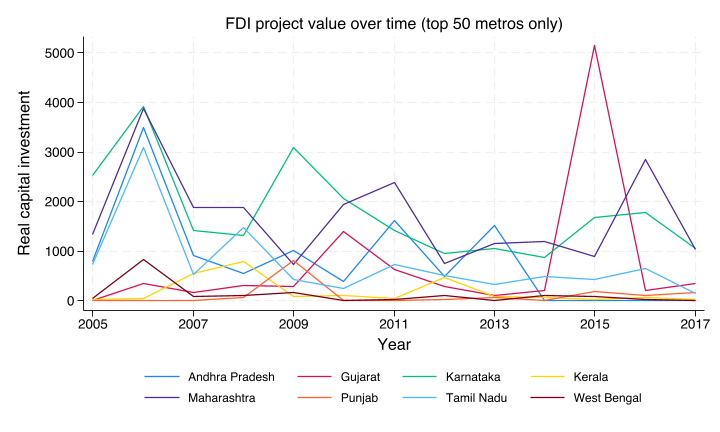
\includegraphics[width=1\linewidth]{4_1_figA8_fdi_value_by_state.png}
            \caption{FDI project value, 2005-2017. Created by author using fDiMarkets data. Note that this has tremendous spikes due to single large projects: the 2015 Gujarat spike is due to SunEdison's \$4 billion investment in Gujarat in 2016 to build India's largest photovoltaic plant, \citep{inc_sunedison_nodate} which is 4 times larger than the next largest investment in our dataset.}
            \label{fig:fdivalue}
        \end{figure}
\begin{figure}
    \centering
    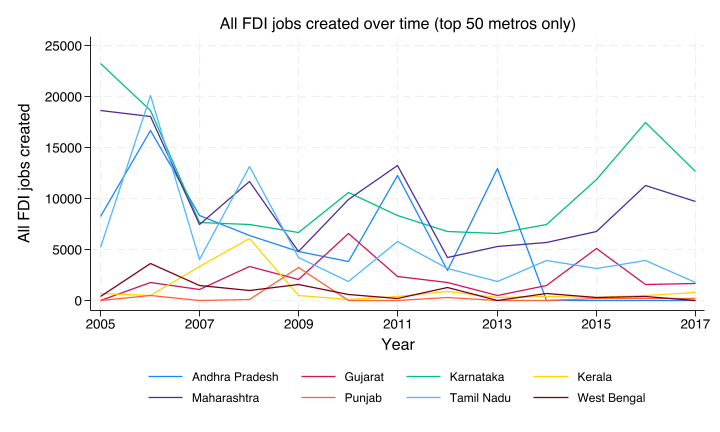
\includegraphics[width=1\linewidth]{4_1_figA9_fdi_jobs_by_state.png}
    \caption{FDI jobs generated, 2005-2017. Created by author using fDiMarkets data. Note this has some reliability issues: SunEdison's announcement of its \$4 billion investment into Gujarat announces that it will create 20,000 jobs (4,500 direct and 15,000 indirect), \citep{inc_sunedison_nodate} but only 3,000 is marked for the project in the data.}
    \label{fig:jobs}
\end{figure}
fDiMarkets also captures sectoral variation in projects. This could be very interesting to investigate if DEPs are more effective for certain types of invesment, e.g. tech investment facilitated by tech workers. As demonstrated below, around half of all FDI projects to India come in the Information and Communications Technology (ICT) sector.
                \begin{figure}
                    \centering
                    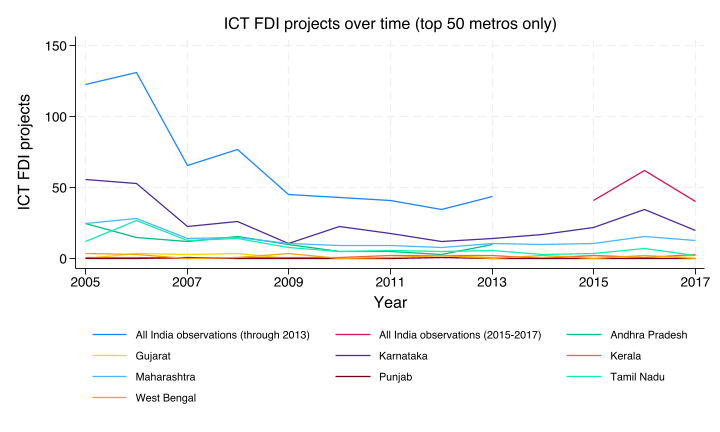
\includegraphics[width=1\linewidth]{4_1_figA10_fdi_ict_projects_by_state.png}
                    \caption{Information and Communications Technology (ICT) projects, 2005-17. Created by author using fDiMarkets data. Note that this is roughly half of all projects in earlier years and 1/3rd in later years.}
                    \label{fig:ictcount}
                \end{figure}
One sector that could potentially be interesting to explore would be retail/consumer goods. In 2012, the Indian government moved from heavy restrictions on retail FDI to allowing for 100\% FDI in single-brand retail and 51\% FDI in multi-brand retail, subject to certain conditions. It would be interesting to interact this shock with DEPs, and see how DEPs either moderate or facilitate them. However, as shown below, this is not something we can currently investigate, as there are at most \~5 retail FDI projects per state/year, and for most states, zero. Any such test would be too underpowered to succeed.
        \begin{figure}
            \centering
            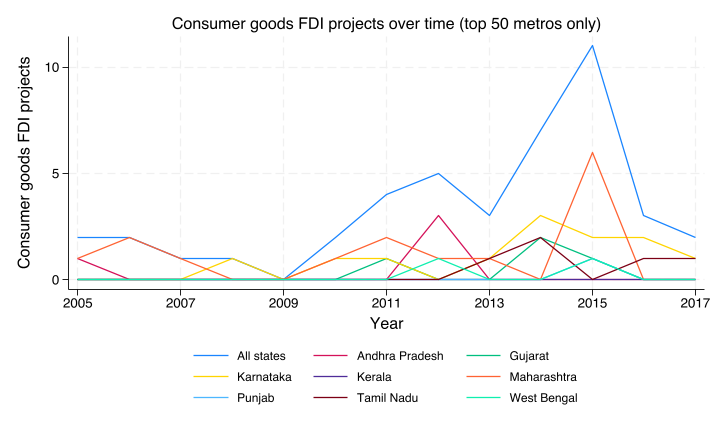
\includegraphics[width=1\linewidth]{4_1_figA11_fdi_consumer_goods_by_state.png}
            \caption{Consumer goods FDI projects, 2005-17. Created by author using fDiMarkets data. Note that there is a marked spike in 2012 and again in 2015 after the liberalization of commercial FDI, but counts in each state are still too low for us to reliably make causal inferences.}
            \label{fig:commercialcount}
        \end{figure}

 \subsection{Operationalizing diasporas} \label{ss:operationalizing diasporas}
            \subsubsection{Strategy} \label{ss:diaspora_measurement_strategy}
We must find a valid and reliable measure of diasporas that gets $e_i$ in $d_i = d_i^* + e_i$ as close as possible to zero. 

A threat to reliability is sampling error. This is when our dataset systemically undercounts or overcounts some segments of the diaspora in the US. To avoid this, I have chosen the US Census Bureau's 1\% samples, as processed by the data provider IPUMS. Each year, the Census Bureau uses a time-tested methodology to collect a sample of 1\% of the US population that is as representative as possible, with minimal sampling error or underinclusion/overinclusion of any group. In addition to correcting Census errors, IPUMS adds on a number of helpful variables to this set, each of which is widely used in the literature. I have confidence that there is minimal sampling error in these data. These 1\% data are available yearly from the year 2000 onward. 

The first threat to validity, meanwhile, is systematic error in the way we define diaspora. As already alluded to, we will be using the Census/IPUMS variable LANGUAGE as a measure of subnational diaspora, with those that report speaking a certain language the most at home being marked as associated with a certain Indian state. There is a large gap between this empirical indicator and the theoretical construct of "subnational diaspora," i.e. someone that feels a strong connection to a certain Indian state.

The second threat to validity is that people who are recorded as speaking the language may not actually affiliate with the Indian state's diaspora, but rather a different state/nation's diaspora. We have already tried to rectify this by only including Indian states that have a highly 1:1 link with US speakers of the language (see Section~\ref{sec:oa_states}). Another source of systematic error is the definition of the LANGUAGE variable itself. LANGUAGE measures the language a respondent spoke at home. This is not a measure of their native language, the language they most identify with, or even just the Indian heritage language that they knew. This is an issue if LANGUAGE undercounts or overcounts certain Indian diaspora groups. For example, Telugu diaspora members could be disproportionately likely to speak Urdu instead at home with their kids, or Tamil second-generation immigrants could be disproportionately likely to stop using Tamil and assimilate. Both those effects of language self-selection and intergenerational language loss are well-documented in the literature, \citep{escobar_indian_2022} making this a massive problem.

One way to mitigate this validity threat is, following in the logic of \citet{mayda_refugees_2022}, disaggregating the diaspora into metro areas. If we simply use the diaspora in the entire US as a measure, we would be comparing the effect of Gujarati non-resident IDs on Gujarati speakers across the entire US vs the effect of Keralan non-resident IDs on Malayalam speakers across the entire US. This would likely be very biased by these language measurement issues. However, if we can just compare the effect of Gujarati non-resident IDs on Gujarati speakers in Los Angeles vs in New Jersey, that would remove a lot of the problems here. This still rests on the assumption that there are no metro-variant measurement errors, like "Gujarati speakers in Los Angeles are more likely to speak Hindi with their kids than Gujarati speakers in New Jersey." Those errors likely still exist: studies find that the coethnic concentration of a metro area matter in language retention by increasing children's heritage language use \citep{chondrogianni_heritage_2023, white_neighborhood_2017}. However, metro disaggregation is likely still better than national aggregation, because national aggregation has a) larger errors, and b) averages over those very different local language-retention environments. 

All in all, LANGUAGE is still our best and realistically only way of identifying subnational diasporas. There will be a number of measures taken throughout the rest of this strategy to minimize its bias. LANGUAGE is only available on a yearly basis from 2005 onward, so that is when we will start our observation.

Let us now discuss more in detail the possible threats from disaggregating into metro areas. One threat to validity here is omitted heterogeneity in the kinds of diaspora members who settle in different places. Our eventual aim is to measure the impact on FDI of the interaction of diasporas $\times$ DEPs. Depending on where they settle, different diaspora groups can have massively different wealth, career paths, and employee statuses that either amplify or diminish the impacts of DEPs on their FDI decision making. This can be a self-selection mechanism: higher-educated Gujaratis can self-select into living in Silicon Valley because that is where all the tech companies are, and then those higher-educated Gujaratis are much more inspired by tax credits to invest back in Ahmedabad. This can also be an environmental mechanism: if two Gujarati twins settle in Silicon Valley and Charlottesville, VA respectively, the Silicon Valley twin is much more likely than the Charlottesville, VA one to start going to college, work for a tech company, and then get inspired by that tax credit. Disaggregating metro areas allows us to apply pair (metro-state) fixed effects to our analysis, allowing us to remove all those time-invariant, metro-specific differences of what kind of Gujarati investors live where.

Another threat to validity here is error in metro area definition. Metro area definition matters because if we undercount or overcount a metro area, we could be skewing some of those crucial fixed effects. Say for some reason we treated Cupertino as separate from the Bay Area. Then, because of all the Apple employees in Cupertino, we would underestimate the fixed effects for the Bay Area (meaning we would overestimate the effects of DEPs on Bay investors), and we would overestimate the fixed effects for whatever metro area we decide to lump Cupertino with (Santa Cruz?). 

There are three metro area measures that IPUMS offers, each with its own flaws. \citep{noauthor_ipums_nodate} The first is METAREA, which uses different metro area delineations from the Office of Management and Budget (OMB) for each decennial Census. This cannot work for our sample, as we are analyzing starting in 2005 and definitely beyond 2010, when the next census took place. Additionally, METAREA "identifies metro areas \textit{only} for residents of areas... that lie entirely within a single metro area. This approach prevents errors of commission (no non-residents of a metro area are identified as residents), but it puts no limit on errors of omission (many residents of metro areas are not identified as residents). METAREA's omissions are widespread and can be very large, occasionally leaving more than half of a metro area's population unidentified." 

The second and third options are MET2013 and MET2023, which use OMB delineations from those years across all years, even back into the 1900s. Those measures ``use an alternative identification protocol that maximizes representativeness. These variables also do not identify any areas where the sum of omission and commission errors would be 15\% or more.'' Since our analysis will stop in 2017 due to FDI data availability reasons, MET2013 is better than MET2023, being closer to most of our observed time period. There is inherent error in any delineation of metro areas. This is only a systematic error if there are disproportionately more errors of commission/omission for some diaspora groups more than others.


    \subsubsection{Separation into samples} \label{ss:samples}
    To ensure our results are robust against those errors, we can run models on different samples. 
    
    One error that we can disaggregate is this idea that diaspora wealth, education, and other baseline characteristics moderate their expected DDI. We can pick out higher education as a especially robust test of this, as whether someone has a college degree determines a lot about what job they work, their wealth \& income, and a whole host of other attributes. We will use the EDUC variable in ACS/IPUMS to create two separate samples here: one of those with a college degree, and one of all diaspora members.
    
    Per our discussion of West Bengal earlier, we will also divide our sample into first-gen diaspora only and all-generation diaspora. Not only does this provide an easy way to include West Bengal, we also will be able to get at if second+-generation diaspora have different effects than non-second-generation-diaspora. 
    
    We will run samples across the following lines:
\begin{enumerate}
    \item Generation (first-gen vs all-gen)
    \item Diaspora education
    \item Diaspora occupation
    \item Age of diaspora (25+, i.e. working adults, vs non-25+)
    \item Type of FDI
    \begin{enumerate}
        \item Sector of company (e.g. information and communication technology vs creative)
        \item Primary activity of the project (e.g. manufacturing vs R\&D)
    \end{enumerate}
\end{enumerate}

   The exact nature of those samples will be detailed later.
   
   \subsubsection{Reliability} \label{ss:samples}
Another issue that emerges is with the reliability of Census/IPUMS data. Because their estimates are 1\% data, how we construct whole-US population numbers is by multiplying each individual's values by their \textit{perwt}, or how many US individuals they are able to represent. This 1\% nature is bad news when dealing with smaller populations like subnational Indian diasporas, as we can have, for example, just 8 people sample out of a 800 population sample.

    For small metro areas, this inserts huge variation into their population estimates per year. This is a global issue that affects all subnational diasporas equally, so this error is not systemic. However, it is still concerning. 
    
    As such, we are restricting our analysis only to the top 50 US metros for each diaspora. This does change how generalizeable our results are: large diaspora metros are likely to differ systematically from small metros in education, industry mix, venture ecosystems, and immigrant network density. Our results will have to be taken as just applying to large metro areas anyways. Luckily, evidence shows that Indian subnational diaspora members tend to overly agglomerate in singular metro areas. For example, nearly 25\% of Gujaratis live in a single metro area (Edison, NJ).

    \begin{figure}
        \centering
        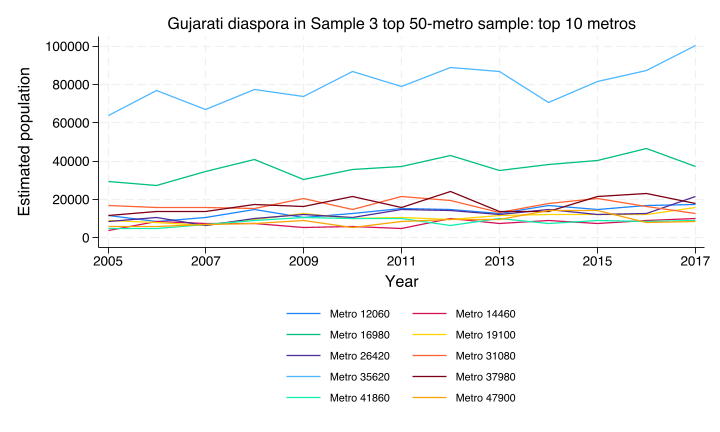
\includegraphics[width=1\linewidth]{4_1_figA12_gujarati_top10_metros.png}
        \caption{Gujarati diaspora (all generations) in its ten largest US metro areas. Restriction to top 50 US metros will reduce generalizability, but that is actually a somewhat minor concern given the tendency of Indian subnational diaspora to agglomerate.}
        \label{fig:sample1 gujarati diaspora}
    \end{figure}
    One potential fix here would have been to use the ACS' 5\% estimates. However, doing so would mean giving up on analyzing events on a yearly level, as ACS explicitly says not to join 5\% estimates on this yearly basis. That is too much of a trade off, so this is the best we can do. 

    \subsubsection{Descriptive statistics of diasporas} \label{ss:diaspora description}
\begin{figure}
    \centering
    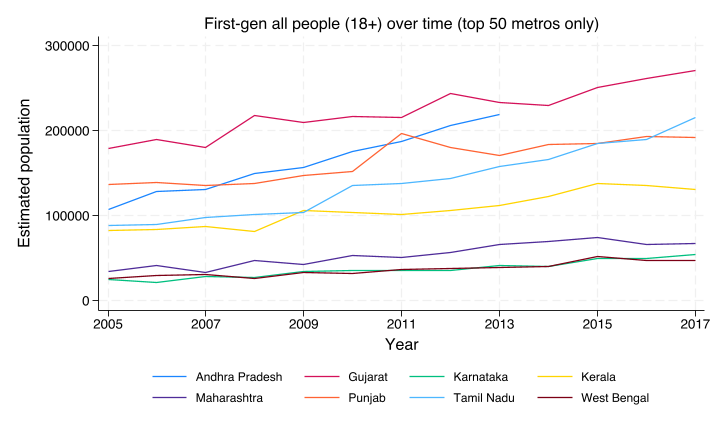
\includegraphics[width=1\linewidth]{4_1_figA13_firstgen_diaspora_by_state.png}
    \caption{First-generation diaspora (born in India) by Indian state, top 50 metros, over time}
    \label{fig:sample1}
\end{figure}
\begin{figure}
    \centering
    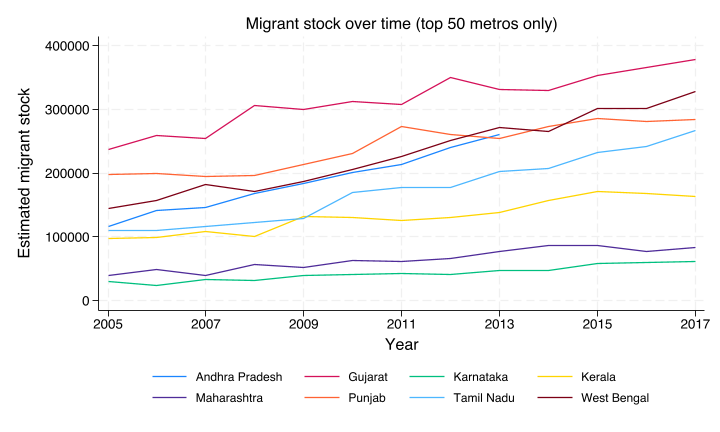
\includegraphics[width=1\linewidth]{4_1_figA14_allgen_diaspora_by_state.png}
    \caption{All-generation diaspora by Indian state, top 50 metros, over time (Bengali speakers of any birthplace included)}
    \label{fig:sample 3}
\end{figure}

\section{DEP Taxonomy, Coding, and Descriptives} \label{sec:oa_deps}

\subsection{Taxonomy}

Figure~\pref{fig:deps_list} in the paper lists all 44 DEPs and the category each belongs to, and Figure~\pref{fig:variable diagram of pathways} shows how the categories map onto the mechanisms of diaspora direct investment.



The list of DEPs and categories is long because it is meant to avoid measurement bias. By being exhaustive of all possible DEPs a state could enact, this paper aims to avoid faulty claims about the efficacy of a category of DEPs that can be disproven with the inclusion or exclusion of a particularly strong or weak DEP.
       \subsection{Operationalizing diaspora engagement policies} \label{ss:operationalizing DEPs}
			In contrast to the other two datasets, the DEP dataset for this project is an original dataset. This dataset consists of 104 state-year observations (8 states across 13 years), with the 44 DEPs in Figure~\pref{fig:deps_list} coded as dummies for each observation.
            Because this is an original dataset, how close $e_i$ in $T_i​=T_i^∗​+e_i$ is to 0 depends largely how we code. Very strict rules were followed in the data generation process to ensure that we would avoid validity issues and have minimal distance between our theoretical construct and empirical indicator. The construct we want to measure is subnational DEPs undertaken by state governments that were actually implemented. To ensure that my measurement matched this construct, I only coded a DEP a 1 if it met the following conditions:
 \begin{enumerate}
     \item \textbf{The policy was implemented by the state government itself. }This excluded many NGOs, civil society organizations, business councils, cultural organizations, etc. that could be considered as fostering diaspora engagement. Even if those organizations received funding from or were partly owned/operated by the government, I did not code those as 1s for the sake of clarity. The only such organizations I included were those fully owned, operated, and advertised as part of the government.\footnote{An investigation of civil society organizations could be helpful in a future paper.} This also excluded policies implemented by local governments like cities, though I could not find many instances of this occurring.
     \item  \textbf{The policy was exclusively targeted towards the subnational diaspora}. This was particularly important for economic policies. Many state policies designed for investor promotion, e.g. single-window facilitation portals, were advertised to and undoubtedly used extensively by the diaspora, but were not designed to give them any special advantage. What is interesting to me is how subnational diaspora agencies can amplify the unique mechanisms of DDI with their policies. Policies not targeted towards the diaspora do not accomplish this.
     \item   \textbf{The DEP did not just exist on paper, but was actually carried out.} Unfortunately, many DEPs are announced by state governments or websites are made, and then no follow-through ever happens. \footnote{Karnataka is the clearest example of this: though it has a DEP website full of promises that were made in 2016, not a single one was ever carried out \citep{noauthor__nodate}. In 2020, over 120 Kannada organizations across 30 countries launched a campaign, \#NRIAPPEALDAY, to call on the Karnataka government to finally install a policy. \citet{noauthor_international_nodate} This campaign is still happening every year.}
 \end{enumerate}

            I went about coding DEPs using a standardized research process:
            \begin{enumerate}
                \item I looked through news announcements, budget speeches, NRI agency websites for announcements of new policies.
                \item I then looked for confirmatory evidence from a trusted source that they had actually ocurred:
                \begin{enumerate}
                    \item Government budgets (the best option)
                    \item Official paper trails from programs (e.g. court documents for NRI police forces)
                    \item Politicians' mentions
                    \item Internet Archive of websites from 2005-2017, confirming that there was a way to actually enroll in the program
                    \item Mentions in official national government documents, generally the Overseas Indian Facilitation Centre (OIFC) or India Center for Migration (ICM)'s documents.\footnote{https://www.mea.gov.in/oia-publications.htm}.
                \end{enumerate}
            \item Secondhand accounts via news articles, social media, etc. were helpful, but I would not code a policy a 1 using those secondhand accounts exclusively unless I found two or more corroborating accounts of the same policy.
            \end{enumerate}

I started by creating state-year audit tables for each state, listing meticulously the first year a policy turned on, if it ever turned off, and listing the evidence for it. Once I finished those audit tables, I then filled out my spreadsheet of dummies.

Despite this meticulous coding process, there are still possible remaining threats to validity and reliability. The first remaining threat to validity is that the dataset may still miss informal or partially institutionalized forms of diaspora engagement. By coding only policies that were implemented by state governments themselves, I gained conceptual clarity, but I may also exclude policies that meaningfully shaped diaspora investment behavior despite not being fully state-owned or formally advertised as government programs. For example, a state-backed business council, diaspora association, or public-private investment forum might plausibly reduce informational or familiarity barriers for diaspora investors even if it does not meet my strict coding threshold. This means that my measure may understate the true level of state-supported diaspora engagement in some state-years. However, this is a conservative validity tradeoff: I prefer to measure a narrower construct clearly rather than include ambiguous quasi-governmental activities that blur the distinction between state policy and civil society activity.

The second remaining threat to validity is that dummy coding may flatten meaningful differences in policy intensity. A state-year is coded as 1 if a policy exists and 0 if it does not, but this does not capture whether the policy was large or small, well-funded or symbolic, actively used or barely maintained. For instance, two states may both have diaspora investment facilitation programs, but one may have a staffed agency, clear application procedures, and regular outreach, while the other may have only a lightly maintained webpage or occasional event. Both would be coded the same way. This creates distance between the theoretical construct of an effective DEP and the empirical indicator of DEP existence. I partially address this by requiring evidence that policies were actually carried out, but the measure still captures the extensive margin of policy adoption more cleanly than the intensive margin of policy strength. Future work could focus on this intensive margin by coding ordinal generosity/restrictiveness scores (0-4 e.g. for how strong a policy is), following in the model of other migration literature like \citet{scipioni_migration_2018}, or correlate this with usage intensity (e.g. how many complaints a grievance redressal policy gets) or budget of a policy. However, those all come with their own issues with standardization across states and validity.

The first remaining threat to reliability is that historical documentation is uneven across states and years. Some state governments preserved budgets, agency websites, policy reports, and archived program materials much more consistently than others. Other states may have implemented policies that left fewer public traces, especially in the earlier part of the sample period. This creates a risk that observed differences in DEPs partly reflect differences in documentation rather than true differences in policy activity. I tried to reduce this risk by using multiple types of confirmatory evidence, including government budgets, official documents, archived websites, and corroborated secondary accounts. Still, because the dataset is original and retrospective, some coding decisions necessarily depend on the survival and accessibility of historical records.

The second remaining threat to reliability is coder judgment. Even with strict coding rules, some policies are difficult to classify because they sit near the boundary between categories. For example, an investment roadshow may also involve business networking, a diaspora conference may include grievance redressal, and an NRI helpdesk may provide both welfare and investment facilitation. To minimize this problem, I used a standardized coding process and coded policies based on their clearest implemented function rather than every possible secondary effect. However, because I am the sole coder, the dataset may still contain some judgment-based inconsistencies. Future work could improve reliability by using multiple coders, calculating intercoder agreement, and adjudicating ambiguous cases through a pre-registered codebook.

\subsubsection{Descriptives of DEPs} \label{subsection:DEPs descriptives}

First, note the total number of DEPs per state increases on average quite substantially over 2005-2017. 

There were some DEPs that did turn off over time. The most notable of those was diaspora conferences, which many states hosted once or twice, but infrequently enough that I could not count it as a recurring DEP.
\begin{figure}
    \centering
    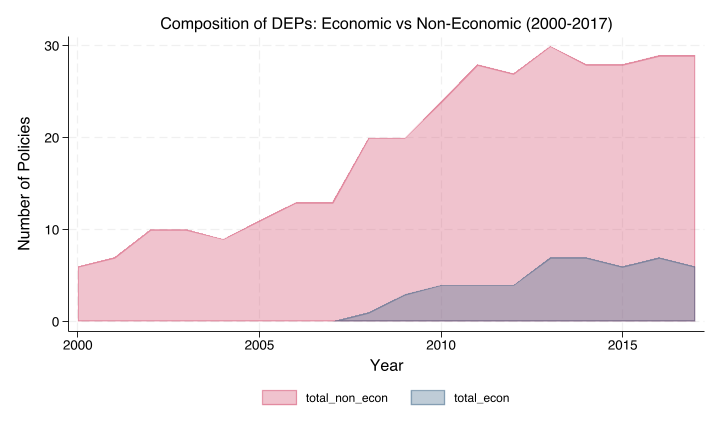
\includegraphics[width=1\linewidth]{4_1_figA15_econ_vs_nonecon_deps.png}
    \caption{Non-econ vs Econ DEPs. Note this is total \# of policies turned on, not total \# of categories of policies turned on. Andhra and Kerala turning on a diaspora admin unit is considered two policies here.}
    \label{fig:Non-Econ vs Econ}
\end{figure}
\begin{figure}
    \centering
    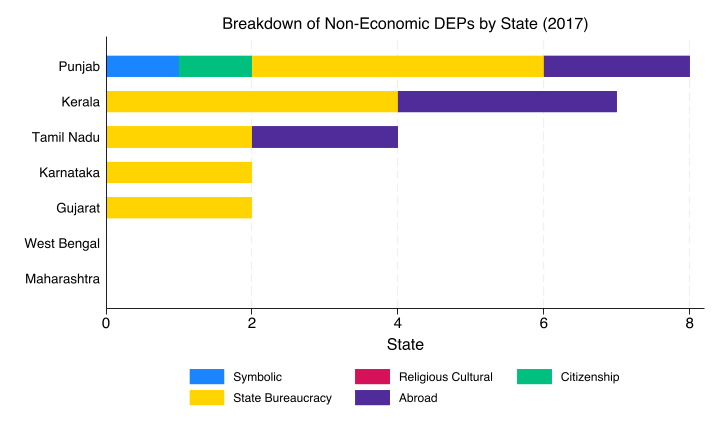
\includegraphics[width=1\linewidth]{4_1_figA16_nonecon_deps_by_state_2017.png}
    \caption{Non-economic DEPs by state in 2017}
    \label{fig:non-econ DEPs by state}
\end{figure}
\begin{figure}
    \centering
    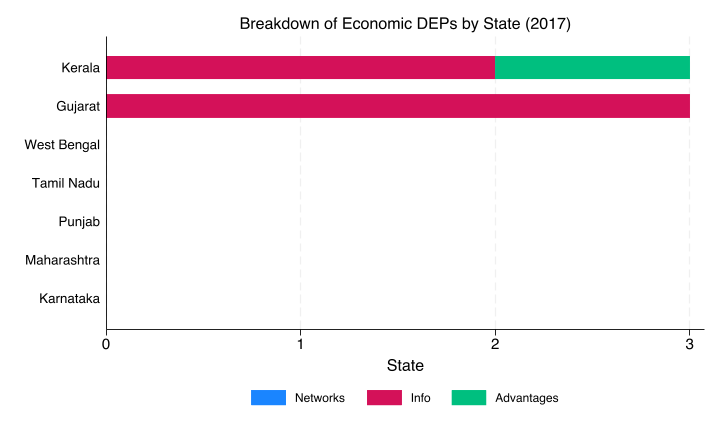
\includegraphics[width=1\linewidth]{4_1_figA17_econ_deps_by_state_2017.png}
    \caption{Economic DEPs by state in 2017}
    \label{fig:econ DEPs by state}
\end{figure}

I also structured my policy buckets to be as mutually exclusive, collectively exhaustive as possible, which is why I have 44 policies. This mutually exclusive part is especially important because having policies that are essentially the same thing would introduce collinearity: if I have both diaspora\_admin\_unit and diaspora\_program\_maintenance, then they would be turned on at the same time for every observation, meaning that inferences would be unstable. I have excluded policies with a high degree of co-adoption.
\begin{figure}
    \centering
    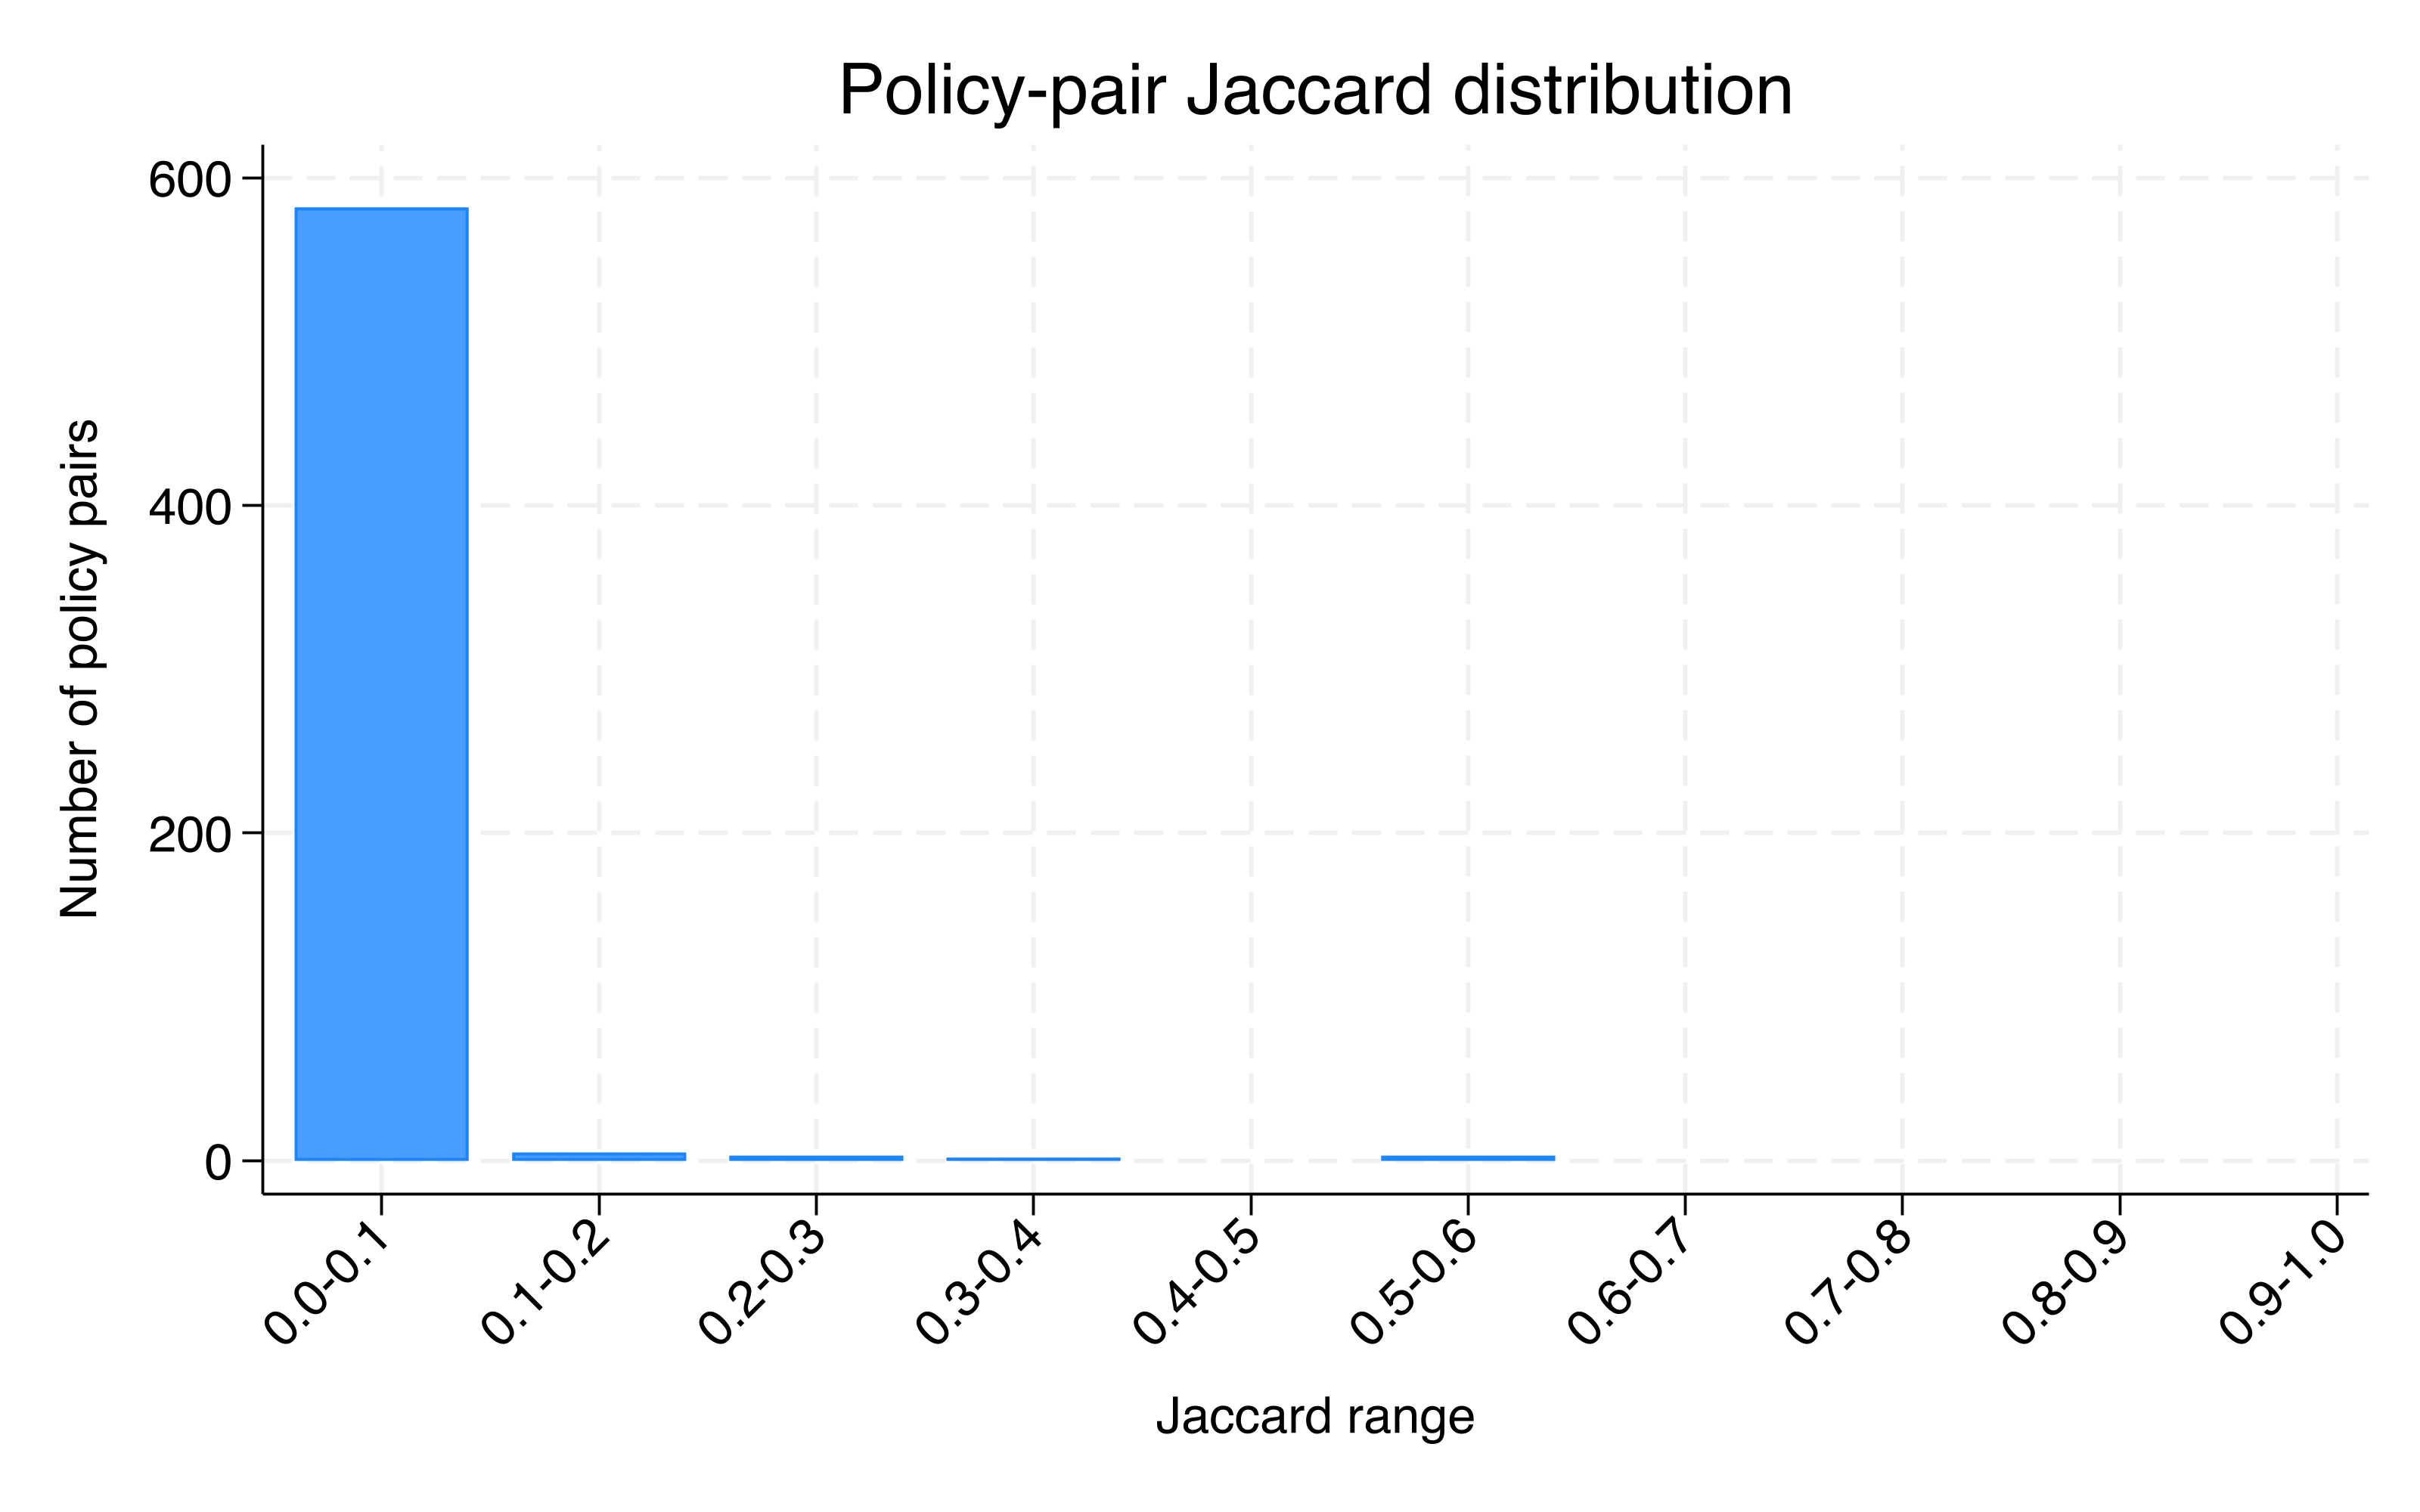
\includegraphics[width=1\linewidth]{4_4_figA18_jaccard_distribution.png}
    \caption{Analysis of policy pairs' Jaccard scores, which refer to how often policies are co-adopted. \citep{jaccard_etude_1901} A score of 1 means that a pair of policies appear together 100\% of the time, while a score of 0.5 means that a pair appears together 50\% of the time. Very few pairs have a Jaccard score higher than 0.1, making co-adoption not a real threat in this sample.}
    \label{fig:jaccard}
\end{figure}
\begin{table}[htbp]
\centering
\footnotesize
\setlength{\tabcolsep}{3pt}
\renewcommand{\arraystretch}{1.08}
\caption{Policy Pairs with the Top 10 Highest Jaccard Scores (Rates of Co-Adoption)}
\label{tab:jaccard_top10}
{\small
\begin{tabular}{r p{2.7cm} p{2.7cm} r r r}
\hline
rank\_jaccard\_pair & row\_item & col\_item & coadopt\_count & union\_count & jaccard \\
\hline
1 & diaspora\_admin\_unit & grievance\_reporting & 2 & 4 & .5 \\
2 & entrepreneurship\_support & tax\_regulatory\_guidance & 1 & 2 & .5 \\
3 & single\_window\_facilitation & tax\_regulatory\_guidance & 1 & 2 & .5 \\
4 & diaspora\_admin\_unit & remains\_repatriation & 1 & 3 & .3333333 \\
5 & grievance\_reporting & remains\_repatriation & 1 & 3 & .3333333 \\
6 & grievance\_reporting & manpower\_companies & 1 & 4 & .25 \\
7 & investment\_promotion\_roadshows & single\_window\_facilitation & 1 & 4 & .25 \\
8 & investment\_promotion\_roadshows & tax\_regulatory\_guidance & 1 & 5 & .2 \\
9 & diaspora\_conferences & investment\_promotion\_roadshows & 2 & 11 & .1818182 \\
10 & diaspora\_conferences & nri\_police & 1 & 9 & .1111111 \\
\hline
\end{tabular}
}
\end{table}


There were cases, however, where policies or policy reform packages fell into two buckets. I would code those cases as a 1 in both buckets. This does introduce some co-adoption risk, but as the Jaccard analysis table shows, the risk is rather minimal. This means that my coding of DEPs is less "how many policies does the state government recognize as separate policies" and more "how many distinct mechanisms does a state government use to engage diasporas." 

    \begin{figure}
        \centering
        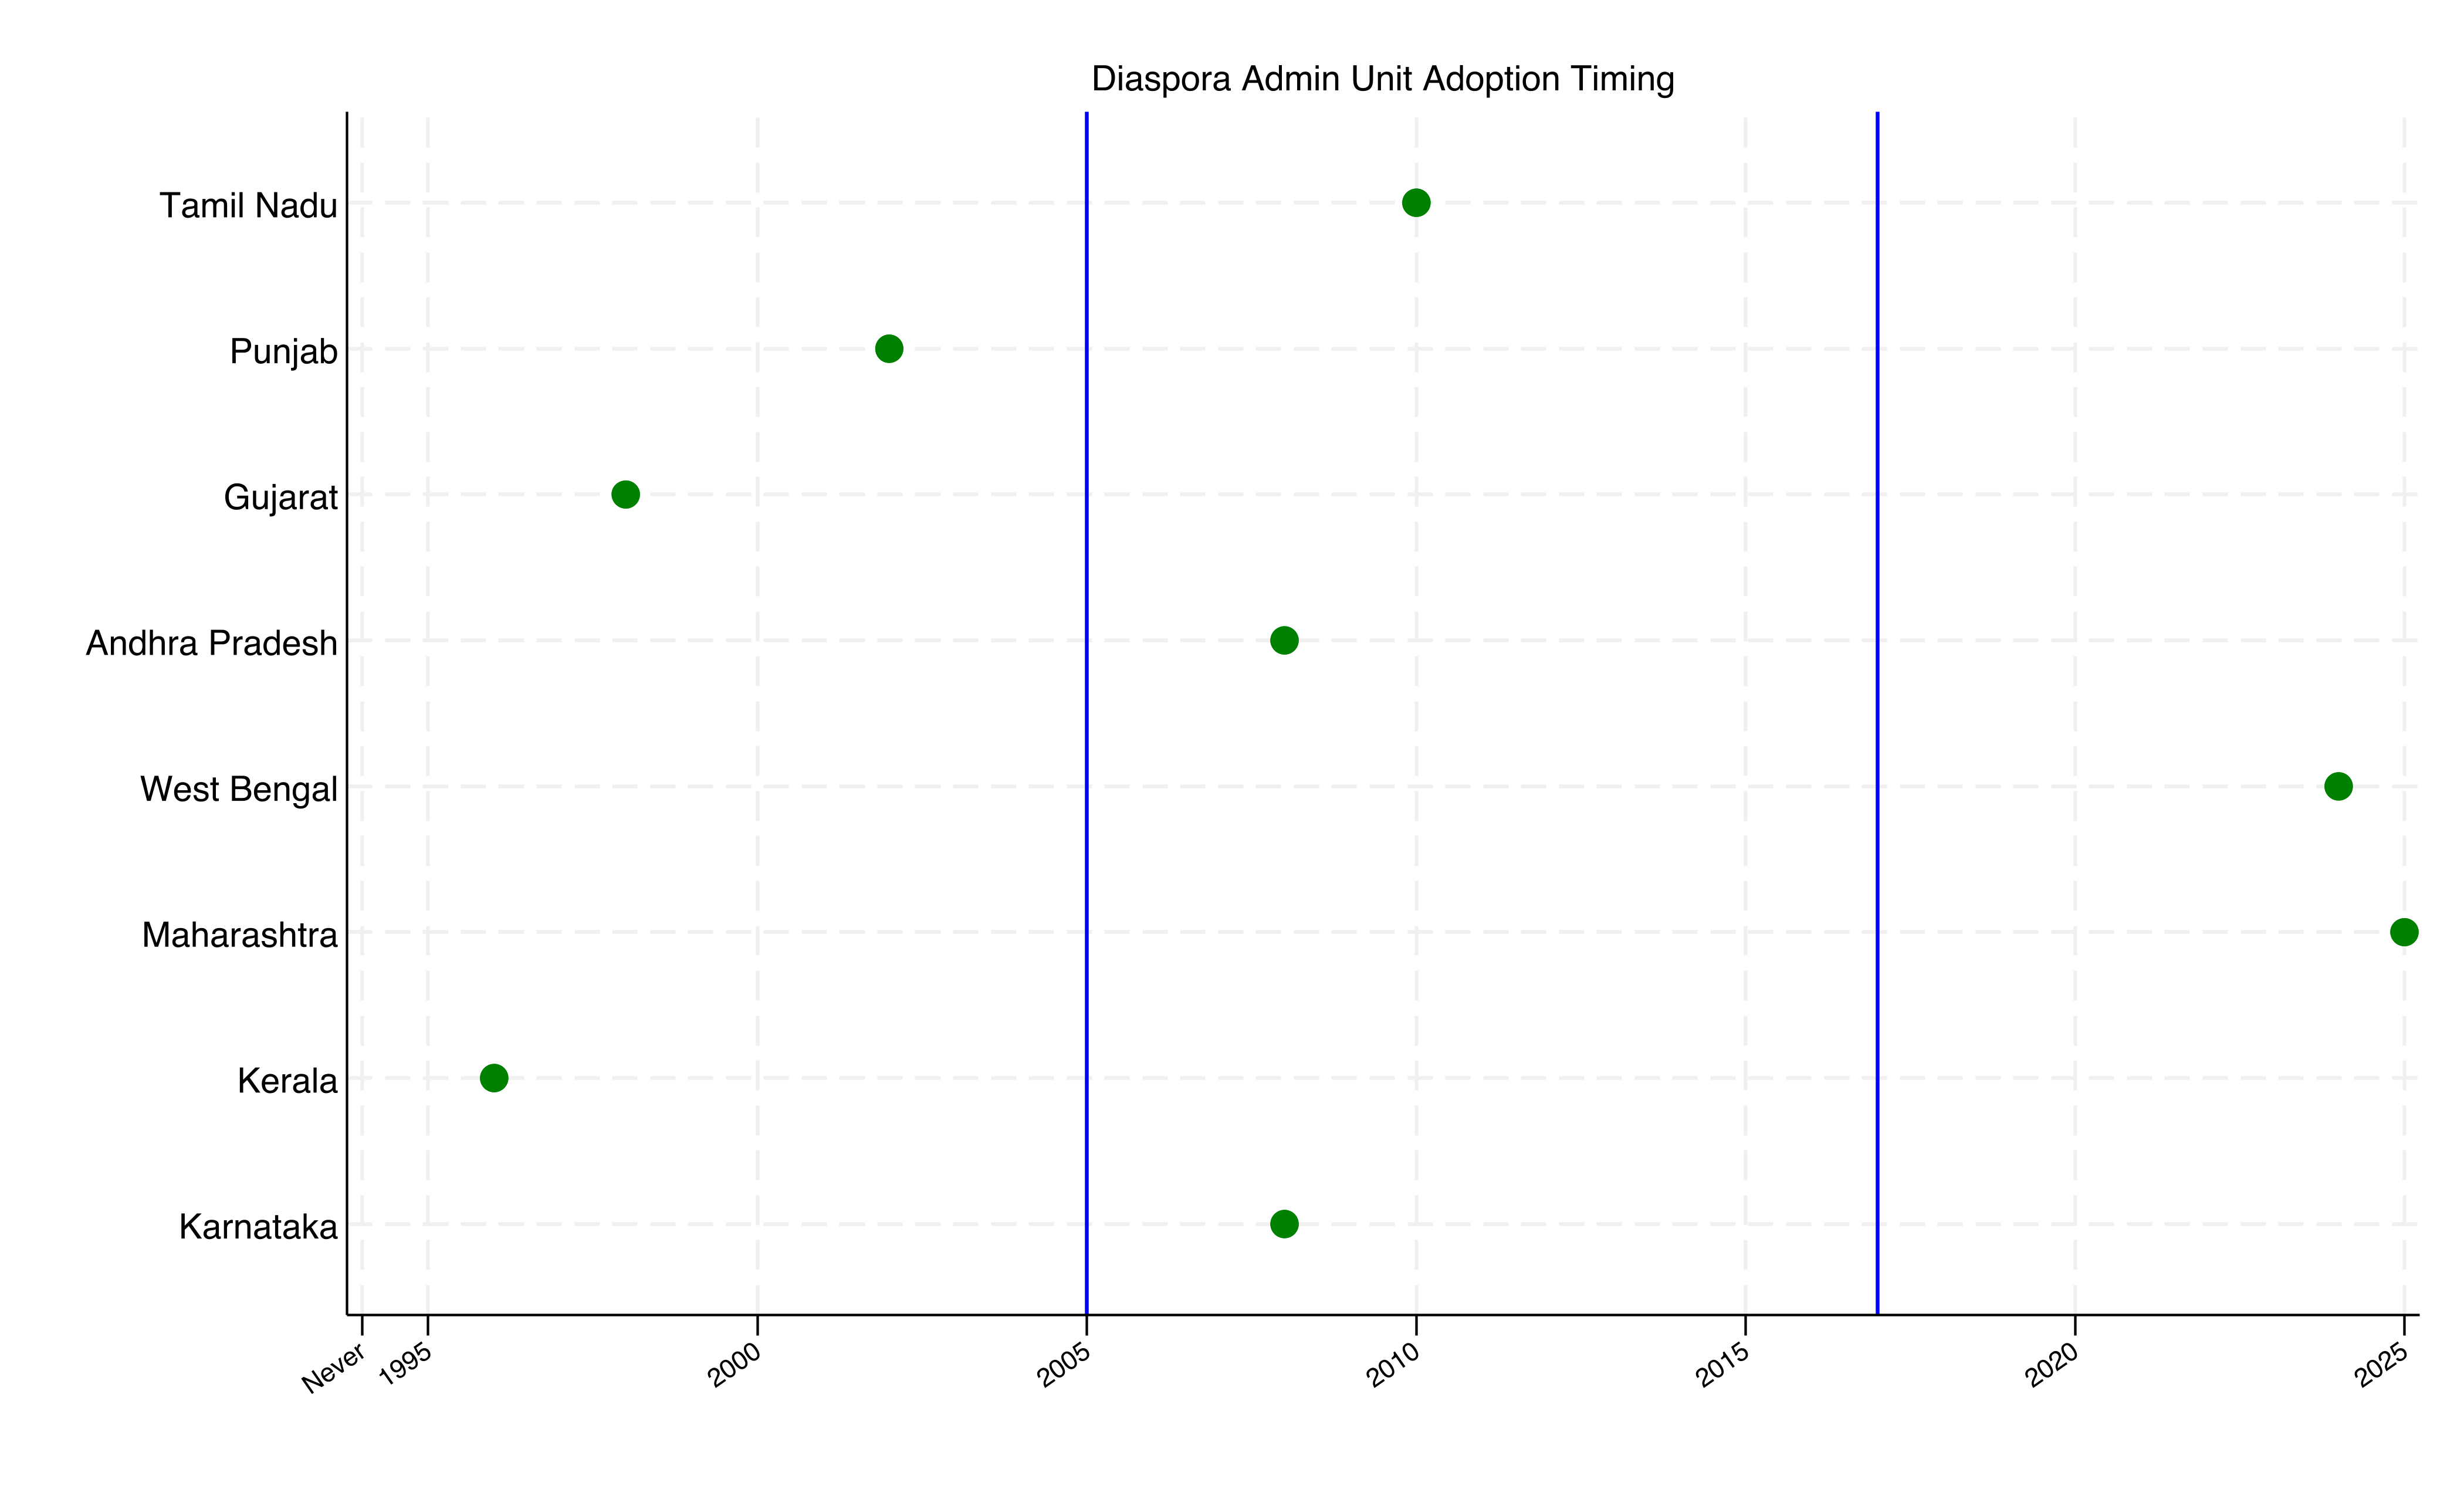
\includegraphics[width=1\linewidth]{4_4_figA19_admin_unit_timing.png}
        \caption{Creation date of governmental diaspora administrative units for each Indian state (note this includes anything from cabinet-level agencies to small working groups).}
        \label{fig:admin_unit_creation_date}
    \end{figure}
    
    As can be seen above, there is no one uniform date where states begin to adopt DEPs. Rather, states adopt DEPs in a staggered manner. This means that India passes our fifth filter of having heterogenous DEP adoption times. Because this case passes all our filters, we can thus discuss how to design our research.

Two more figures describe economic DEPs specifically: how economic DEP types grow over time, and when each state first adopted each informational DEP.

\begin{figure}
    \centering
    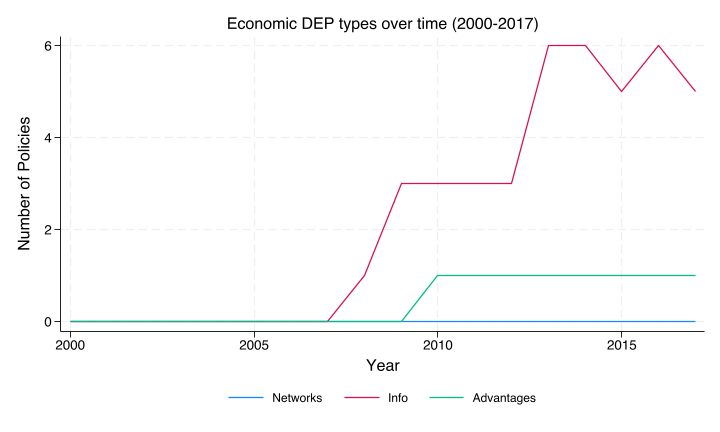
\includegraphics[width=1\linewidth]{4_1_figA20_econ_dep_types.png}
    \caption{Economic DEP types over time}
    \label{fig:econ DEP types over time}
\end{figure}
\begin{figure}
    \centering
    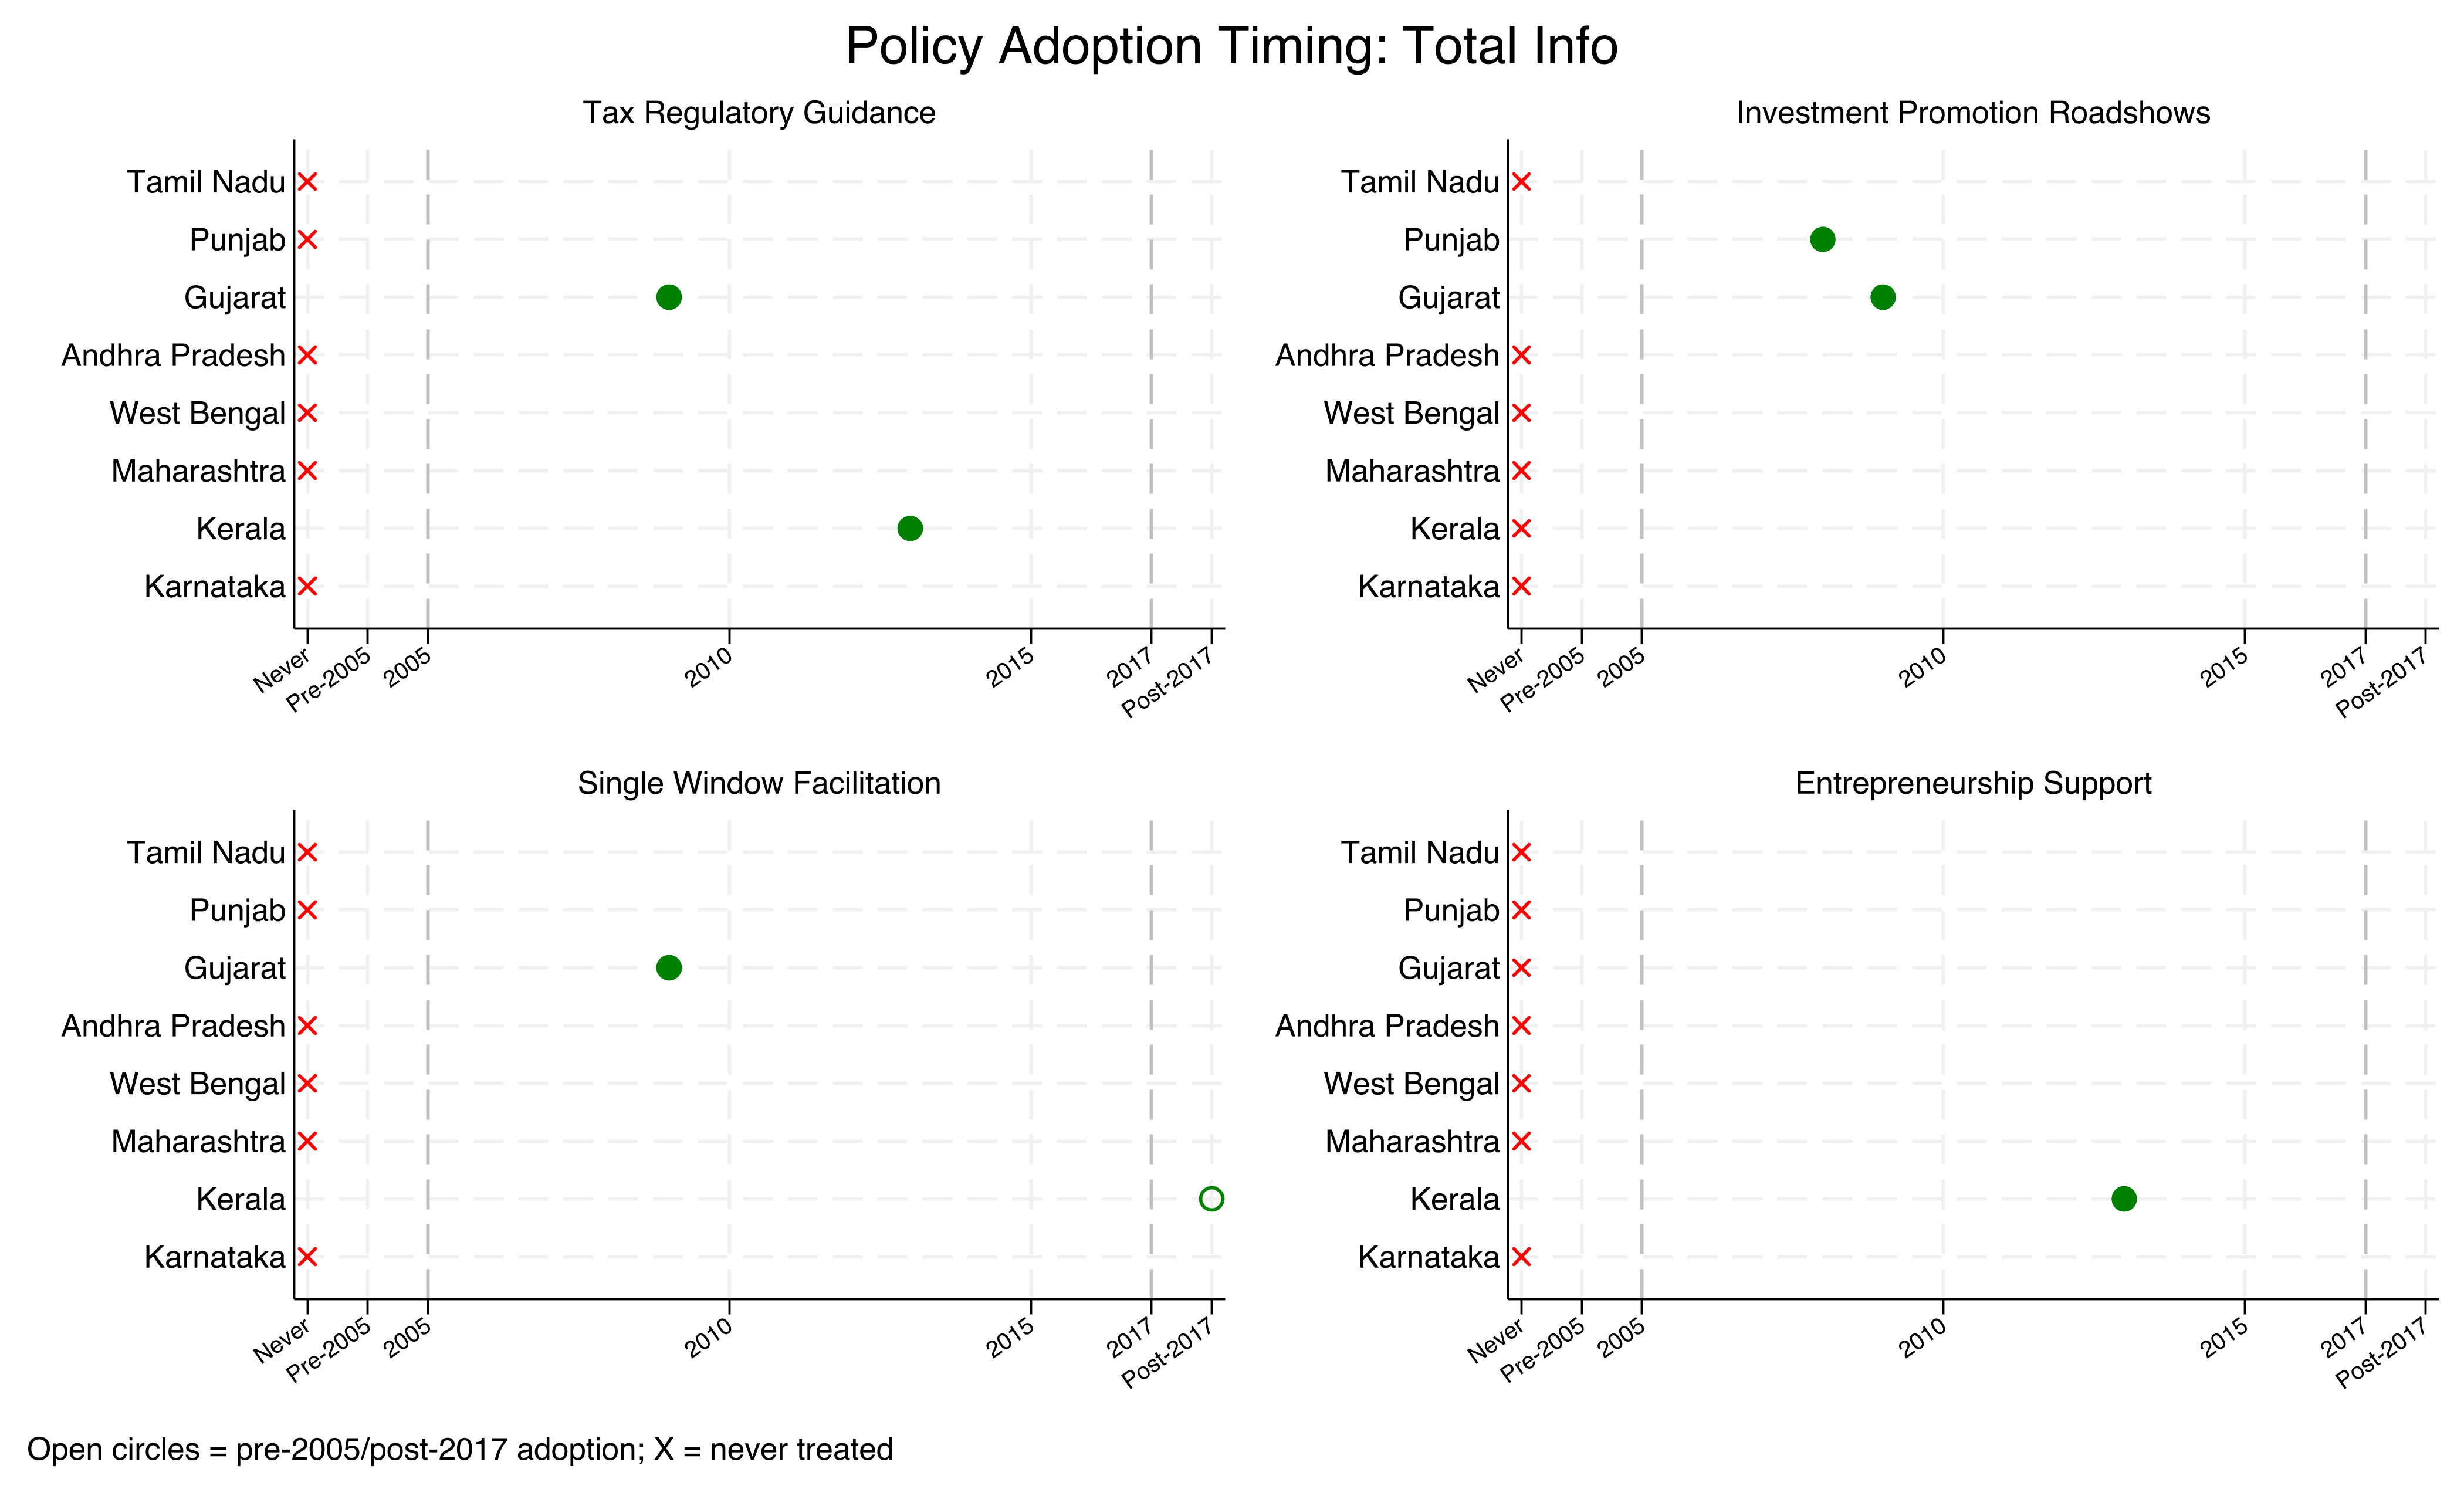
\includegraphics[width=1\linewidth]{4_4_figA21_info_policy_timing.png}
    \caption{Adoption timing of informational DEPs by state. Filled circles mark adoption in 2005--2017, open circles adoption before 2005 or after 2017, and X marks states that never adopted the policy.}
    \label{fig:info_timing}
    \end{figure}

\section{Estimation and Identification Details} \label{sec:oa_identification}

This section gives the full version of the estimation and identification discussion in Section~\pref{sec:strategy} of the paper.

    The goal of research design is to do two things. First is identification, or what causal or descriptive quantity we are trying to learn, and what assumptions let our observed data remove the bias term and recover it. Second is estimation, which is which model we select to implement those assumptions. In order to talk about our identification issues in a non-abstract way later, let us first begin with estimation.

\subsection{Estimation: Why PPML?} \label{ss:why_ppml}
    
   Following in the extant literature on FDI, the only estimator I use in this paper is Poisson pseudo-maximum likelihood (PPML \citep{li_repelling_2026}). This is because the outcome is a count, this is a 'gravity-based' situation, and the data have many zeros.
    
    A Poisson distribution is a type of probability distribution for count variables exclusively (i.e. those that cannot be expressed in decimals and cannot be negative). It describes how likely we are to observe 0, 1, 2, etc. of some event in a fixed unit of time, space, or another observational cell. The classic examples are how many calls a help desk gets per hour, how many accidents happen at an intersection per month, or how many customers arrive at a store per day.  Here, this is how many FDI projects go from US metro $m$ to Indian state $s$ in year $t$. 

    
    The key idea with Poisson is that, unlike with a standard normal distribution, we are not measuring a continuous quantity, but rather the number of times something happens. In the simplest Poisson setting, there is some average rate at which events occur, and the distribution tells us the probability of observing different count values around that average. If the expected number of events is low, zeros and ones are common. If the expected number is high, larger counts become more likely. The standard Poisson regression model takes that intuition and lets the expected count vary with observed covariates. It assumes that the conditional mean is positive and can be written as an exponential function:
\[
E[Y_{mst} \mid X_{mst}] = \exp(X_{mst}\beta).
\]

Poisson is commonly used for gravity models. A gravity model, named so because it borrows from the Newtonian concept of gravity, explains flows (trade, FDI,  remittances, etc.) between two places as a function of connection and barriers. Just like in physics, flows rise when two places are larger or more connected, and fall  when barriers between them are higher.   In my context, the flow is the number of FDI projects from US metro $m$ to Indian state $s$ in year $t$. The ``mass'' or connection between those places is partly captured by the size of the relevant subnational diaspora in metro $m$, while the barriers are the informational, bureaucratic, legal, and familiarity costs that make investing in a particular Indian state difficult.

Poisson's exponential conditional-mean structure makes it especially natural for gravity models like mine. Taking logs of the Poisson mean gives
\[
\log E[Y_{mst} \mid X_{mst}] = X_{mst}\beta,
\]
so each covariate shifts the expected flow in percentage-like terms rather than by adding a fixed number of projects. This is good because FDI flows are likely to scale multiplicatively, not additively. A larger diaspora probably does not add the same fixed number of FDI projects to every metro-state pair. Instead, it likely changes the expected rate of investment proportionally, with larger effects in dyads where baseline investment is already larger. Similarly, if DEPs reduce informational, bureaucratic, legal, or familiarity barriers, they should make investment more likely by lowering the effective cost of investing in that state, not by mechanically adding the same number of projects to every dyad.

    This model is multiplicative and not additive, because in these models, variables typically scale flows proportionally, not additively. For example, if a larger diaspora doubles expected FDI rather than adding exactly 0.7 projects to every metro-state pair, that is multiplicative. Similarly, if a policy raises expected investment by 20\%, that is naturally multiplicative, not linear. This is why FDI researchers often start with this Poisson gravity mean.

    One useful thing is that Poisson can deal with many zeroes, as is common in trade/FDI settings. Most cells in my data of metro $m$ $\times$ Indian state $s$ $\times$ year $t$ have zero FDI projects, while a smaller number have one or more. Older gravity models often used OLS and just logged the dependent variable. But $\log(0)$ does not exist. Additionally, in this dataset, zeros are meaningful. If Punjabi-heavy Los Angeles sends zero FDI projects to Punjab in 2009, that is substantively meaningful. Dropping those observations would mean throwing away exactly the information that tells us whether DEPs actually change the extensive margin of investment.

    An additional useful thing about this type of Poisson gravity model is that it cannot predict negative FDI projects. OLS can, because OLS is just fitting a line. Poisson cannot, because exponentials are always positive. 

    A note is that PPML does not require the outcome to literally follow a perfect Poisson distribution. This is where the ``pseudo'' part matters. In a literal Poisson distribution, the mean and variance are equal. FDI project counts almost definitely violate that. There are too many zeros, and investment arrives in lumps. But PPML only needs the conditional mean to be correctly specified, not the full distribution \citep{gourieroux_pseudo_1984, wooldridge_distribution-free_1999}. This is why \citep{santos_silva_log_2006} argue for PPML in gravity models. According to them, OLS is biased in situations where the real data generating process is multiplicative. It is also biased in heteroskedastic situations (i.e. when the variance changes systematically across observations -- say, high-FDI metro-state dyads have more variance than low-FDI dyads). Meanwhile, PPML can remain consistent under weaker assumptions. 

\subsection{Estimation: PPML Specification} \label{ss:specification}

We will be using two PPML specifications, one for $H_0$, and one for $H_{1-3}$. 

In both, $Y_{mst}$ is the count of FDI projects from US metro $m$ to Indian state $s$ in year $t$. $Diaspora_{mst}$ is the relevant diaspora population in US metro $m$ associated with Indian state $s$ in year $t$, measured from ACS/IPUMS. $DEP_{st}$ is the state-year DEP variable. Depending on the model, it is either an any-policy indicator, a total policy count, or an active individual policy variable.

For \textbf{$H_0$:  As the location-specificity of a diaspora group increases, the positive effect it has on foreign direct investment to that location increases}, I will use:
\[
E[Y_{mst} \mid X_{mst}] =
\exp \Bigl(
\beta_1 \ln(1+Diaspora_{mst})
\Bigr).
\]
We will be running this on both subnational diasporas and the broader Indian diaspora for each metro area, then doing a simple  comparison of $\beta_1$ in both. For this specification, I will be clustering at the metro level. This is because the treatment (location-specificity of the diaspora group) is being applied at the US metro level, meaning that if we did not cluster, we would assume more independent variation than there actually is.

For \textbf{$H_{1-3}$, which are concerned with adoption of any DEP ($H_1$), total number of DEPs ($H_2$), and the degree of economic advantage given by a DEP ($H_3$)}, I will use:
\[
\begin{aligned}
E[Y_{mst} \mid X_{mst}] =
\exp \Bigl(
&\beta_1 \ln(1+Diaspora_{mst}) \\
&+ \beta_2 DEP_{st} \\
&+ \beta_3 \left[\ln(1+Diaspora_{mst}) \times DEP_{st}\right] \Bigr).
\end{aligned}
\]
For this specification, I will be clustering at the Indian state level, because the treatment (states' DEPs) are being applied at the state level. Note that this leaves us with only 8 clusters (8 Indian states), which means that any inferences will be fragile. We must thus be cautious about interpreting borderline p-values, and emphasize effect direction, magnitude, and consistency instead of just significance.

Note that our $H_{1-3}$ specifications are single-policy estimates on DEPs, not multi-policy estimates. Single-policy estimates simply swap out one DEP/one DEP category for another in the DEP term. Econometrics literature states to use this in situations where the main goal is a clean reduced-form estimate for one treatment at a time rather than decomposition across overlapping treatments \citep{goldsmith-pinkham_estimating_2021}. Our $H_{1-3}$ specifications fit this bill because they estimate very separate treatments: any DEPs at all, total number of DEPs, and very separate categories of DEPs. I have also attached a table that uses a single-policy version of our DEP PPML specification to estimate individual policy coefficients in Section~\ref{sec:oa_results}.

Multi-policy estimates, meanwhile, add \textit{all} DEPs to our regression. Econometrics literature states to use this only if we have a \textit{small} number of conceptually distinct policy variables and you want the incremental effect of each, conditional on the others \citep{yotov_advanced_nodate}. Because we have 40+ policies, we cannot very accurately estimate the effects of individual policies using a multi-policy estimate. 

A final note is that running a triple interaction with one of India's two FDI liberalizations -- 2005 and 2012 -- would be a massive boon to causal identification. Unfortunately, we are simply constrained by data for 2005: we do not have project-level FDI data from before 2005. Even if we did have this data, there were only 3 states with DEPs in 2005 (Gujarat, Punjab, and Kerala), none of which were large FDI recipient states, and only 10 DEPs active. Causal identification would be very difficult in this setting. The 2012 retail liberalization, meanwhile, did lead to a spike in consumer goods projects, but there are simply too little consumer goods projects in our sample to make inferences, and any consumer goods spikes would get drowned out by the non-movement of all-sector FDI in that time period.

We will be using \citet{correia_fast_2020}'s widely used Stata package, ppmlhfde, to estimate our regressions. ppmlhfde stands for (pseudo-)Poisson regression models with multiple high-dimensional fixed effects (HDFE).

\subsection{Identification: Fixed Effects}

The models described above are simple, and do not control for many omitted variables that are time-variant and invariant. We can use fixed effects to wash out a lot of those omitted variables. Let us discuss our two models with fixed effects:

For \textbf{$H_0$:  As the location-specificity of a diaspora group increases, the positive effect it has on foreign direct investment to that location increases}, I will use:
\[
E[Y_{mst} \mid X_{mst}] =
\exp \Bigl(
\beta_1 \ln(1+Diaspora_{mst})
+ \alpha_{m}
+ \delta_{st}
\Bigr).
\]

Here for $H_0$, we are using state-year fixed effects, $\delta_{st}$; and \textbf{\textit{metro}} fixed effects, $\alpha_{m}$. State-year fixed effects absorb all factors common to a given Indian state in a given year, including both persistent state differences and state-specific shocks in that year. This will also wash out any time-invariant differences between US metros (e.g. if San Francisco is more tech oriented than Little Rock, Arkansas).

We cannot use metro-year fixed effects here because total Indian diaspora size would be perfectly collinear with those FE: it only varies at the metro $\times$ year level. Subnational diaspora size varies at the state $\times$ metro $\times$ year level and so we can use metro-year here, but for the sake of comparison with Indian national diaspora, we will exclude them. As such, this does not capture metro-year shocks that may hit different metros differently (e.g. the 2008 recession). 

For \textbf{$H_{1-3}$, which are concerned with adoption of any DEP ($H_1$), total number of DEPs ($H_2$), and the degree of economic advantage given by a DEP ($H_3$)}, I will use:
\[
\begin{aligned}
E[Y_{mst} \mid X_{mst}] =
\exp \Bigl(
&\beta_1 \ln(1+Diaspora_{mst}) \\
&+ \beta_2 DEP_{st} \\
&+ \beta_3 \left[\ln(1+Diaspora_{mst}) \times DEP_{st}\right] \\
&+ \alpha_{ms}
+ \gamma_{mt}
+ \delta_{st}
\Bigr).
\end{aligned}
\]

Here, I will be using state-year fixed effects; $\delta_{st}$; \textbf{\textit{metro-year}} fixed effects, $\gamma_{mt}$; and metro-state \textbf{dyad} fixed effects, $\alpha_{ms}$. Note the change from using metro FE in $H_0$ to metro-year FE in $H_{1-3}$: because we are looking at subnational diasporas and not the national Indian diaspora, we can now deploy these FE. This captures not just all time-invariant differences between metros, but also any metro-year shocks, like a tech boom in San Francisco. Dyad FE lets us net out time-invariant bilateral factors: persistent metro-state affinity, historical business ties, etc. 

What these fixed effects do not absorb are metro-state-year shocks, or state-level shocks whose effects differ systematically across metro-state dyads. For example, if Andhra Pradesh implements a general investment facilitation policy in 2008, and that raises FDI by +8 in high-diaspora metro-state dyads, and only by +3 in low-diaspora dyads, that differential effect would not be removed by metro-year, state-year, and dyad fixed effects alone. In other words, these fixed effects absorb additive metro-year and state-year confounders, but not confounders that operate through the diaspora-exposure margin itself. We will discuss strategies to combat these \textit{diaspora-skewed} shocks later.

\subsection{Identification: Bundled \& Rare Policies } \label{ss: bundled, rare policies}

There are a number of threats posed by the structure of our DEP data to testing of $H_{1-3}$ specifically.

As already discussed in the DEP measurement section, the first possible threat is bundling: if a state creates multiple DEPs in the same reform package, we may not be able to separate the effect of each component cleanly. This matters most for policy-type and individual-policy estimates. For example, if a state adopts diaspora conferences, investment roadshows, and matching funds in the same year, then a coefficient on one of those policies may partly reflect the broader package rather than that instrument alone. The design therefore identifies the net effect of a state-level DEP environment more cleanly than it identifies the independent causal effect of each policy component.

This distinction is less problematic for $H_1$ and $H_2$. Those hypotheses are explicitly about the extensive and intensive margins of DEP adoption: whether having any DEP, or having more DEPs, changes the relationship between diaspora size and FDI. For those models, a bundled reform package is part of the treatment itself. It becomes more important for $H_3$ and the individual-policy appendix, where coefficients should be interpreted as reduced-form associations with policy types rather than fully separable causal effects of each instrument.

Empirically, however, bundling appears limited in this dataset. The Jaccard tables show that only a small number of policy pairs co-adopt to a meaningful degree, and the adoption-timing table does not reveal many large simultaneous reform packages. The largest same-year package contains three DEPs. Thus, bundling may move the interpretation of the more disaggregated estimates for a select few policies, but it is unlikely to drive the main $H_1$ and $H_2$ findings entirely.

\begin{table}[htbp]
\centering
\caption{Timing and Bundling of New Diaspora Engagement Policies across Indian States, 2005--2017}
\label{tab:dep_turnon_events}
\scriptsize
\setlength{\tabcolsep}{2pt}
\renewcommand{\arraystretch}{1.08}
\begin{tabularx}{\textwidth}{@{}l *{8}{>{\RaggedRight\arraybackslash}X}@{}}
\hline
\textbf{Year} & \textbf{Andhra Pradesh} & \textbf{Gujarat} & \textbf{Karnataka} & \textbf{Kerala} & \textbf{Maharashtra} & \textbf{Punjab} & \textbf{Tamil Nadu} & \textbf{West Bengal} \\
\hline
2005 & 0 & 0 & 0 & \makecell[tl]{2: Diaspora\\Conferences,\\Welfare\\for\\Returnees} & 0 & 0 & 0 & 0 \\
\hline
2006 & \makecell[tl]{1: Manpower\\Companies} & 0 & 0 & \makecell[tl]{2: Grievance\\Reporting,\\Manpower\\Companies} & 0 & 0 & 0 & 0 \\
\hline
2007 & 0 & 0 & 0 & 0 & 0 & 0 & 0 & 0 \\
\hline
2008 & \makecell[tl]{2: Diaspora\\Admin\\Unit,\\Grievance\\Reporting} & 0 & \makecell[tl]{1: Diaspora\\Admin\\Unit} & \makecell[tl]{2: Diaspora\\Conferences,\\Origin\\ID\\for\\Non-Citizens} & 0 & \makecell[tl]{2: Diaspora\\Conferences,\\Investment\\Promotion\\Roadshows} & 0 & 0 \\
\hline
2009 & 0 & \makecell[tl]{3: Tax\\Regulatory\\Guidance,\\Investment\\Promotion\\Roadshows,\\Single-Window\\Facilitation} & 0 & 0 & 0 & 0 & 0 & 0 \\
\hline
2010 & 0 & 0 & 0 & \makecell[tl]{1: Loan\\Advantages} & 0 & 0 & \makecell[tl]{3: Diaspora\\Admin\\Unit,\\Grievance\\Reporting,\\Remains\\Repatriation} & 0 \\
\hline
2011 & 0 & 0 & \makecell[tl]{1: Diaspora\\Conferences} & \makecell[tl]{1: Diaspora\\Conferences} & 0 & \makecell[tl]{2: Diaspora\\Conferences,\\NRI\\Police} & 0 & 0 \\
\hline
2012 & \makecell[tl]{1: Diaspora\\Conferences} & 0 & 0 & 0 & 0 & \makecell[tl]{1: Other\\Predeparture\\Support} & 0 & 0 \\
\hline
2013 & 0 & 0 & 0 & \makecell[tl]{2: Tax\\Regulatory\\Guidance,\\Entrepreneurship\\Support} & 0 & \makecell[tl]{2: Diaspora\\Conferences,\\Investment\\Promotion\\Roadshows} & 0 & 0 \\
\hline
2014 &  & 0 & 0 & 0 & 0 & \makecell[tl]{1: NRI\\Courts} & 0 & 0 \\
\hline
2015 &  & 0 & 0 & \makecell[tl]{2: Diaspora\\Conferences,\\NRI\\Courts} & 0 & 0 & 0 & 0 \\
\hline
2016 &  & 0 & \makecell[tl]{1: Improved\\Statistics\\Reports} & 0 & 0 & \makecell[tl]{1: Investment\\Promotion\\Roadshows} & 0 & 0 \\
\hline
2017 &  & 0 & 0 & 0 & 0 & \makecell[tl]{1: Diaspora\\Affinity\\Proclamation} & 0 & 0 \\
\hline
\end{tabularx}

\vspace{0.4em}
\begin{minipage}{0.97\textwidth}
\scriptsize
\textit{Notes:} Entries report diaspora engagement policies (DEPs) that switch on in a given state-year. Cells beginning with a number indicate the count of newly adopted policies, followed by the specific policy names. A value of 0 indicates no new policy adoption in that year. Blank Andhra Pradesh cells in 2014--2017 reflect the state bifurcation period and corresponding coding treatment.
\end{minipage}
\end{table}


Another possible threat is rare policies. If a policy only turns on in one state or one year, PPML can still estimate something, but it is much more like a case-study contrast than a reliable panel estimate. We will exclude rare policies (identified as those either adopted by less than 2 states or for less than 10 state-years) from $H_2$ and $H_3$. In our appendix table of individual policy estimates, we will also list tiers of policies by how rare they are (3+ states and 20 + state-years; 2+ states and 10+ state-years; less).

\subsection{Identification: Model Mechanics } \label{ss: model mechanics}

There are two features of our model that are meant to prevent bias, but we must also ensure that those features do not become sources of bias themselves.

The first is PPML's separation handling. Separation is when some observations make the likelihood want to send a coefficient or fixed effect toward positive or negative infinity. This happens when certain combinations of regressors and FE perfectly predict zeros or perfectly isolate a pattern the model can fit only with an extreme parameter. 

ppmlhdfe was built to handle separation, but it does so by dropping observations that cause it. ppmlhfde also drops singletons (fixed effects groups that only appear once). The net effect of these drops is that we often end up with smaller samples in PPML than we begin with. To ensure that my estimates are not being created off tiny samples, I report for every sample the number of observations pre-drop, number we are left with post-drops, number of singletons, and number of separated observations.

Another threat to identification that emerges from our PPML specification is small-cluster inference. As previously discussed, we only have 8 states/clusters on $H_{1-3}$, making inferences fragile. As we have mapped out in our criteria for selecting states (see Section~\ref{sec:oa_states}), there is unfortunately no justifiable way to increase the number of state observations. As such, this is the best that we can do.

\subsection{Identification: Reverse Causation} \label{ss:logical threats}

We have concluded our discussion of how the structure of our data and specification itself may pose a threat to identification. We will now turn our attention to the identifying assumption of PPML.

The identifying assumption of PPML is that after conditioning on metro-state FE, metro-year FE, state-year FE, and our included regressors, there are no omitted shocks correlated with the regressor of interest. A violation of this assumption would represent $Estimate \neq Estimand$ because the $Bias$ term,  $\left[\bar{\Delta}_T(0)-\bar{\Delta}_U(0)\right]$ is not 0. In words, this is when states that adopt DEPs would be different on FDI than states without DEPs even without the DEPs. We will walk through ways in which this may happen.

First, reverse causation is a threat. If states adopt DEPs in response to rising FDI, our estimates could actually reflect states that adopt DEPs having higher untreated paths and not the causal effect of DEPs. 
We can evaluate this by comparing FDI data with the amount of DEPs adopted over time. On the FDI trends, we note that there is a large spike in 2006 after the 2005 FDI liberalization, followed by a taper off across 2011-2017. States may have expected higher FDI either after 2005 or after the 2012 liberalization of consumer good FDI.  On the DEP trends, we note that some states do adopt more DEPs around this time: Gujarat turns on tax \& regulatory guidance and roadshows around 2009, Andhra turns on diaspora admin unit and grievance reporting in 2008, and Punjab turns on diaspora conferences, investment roadshows, and matching funds in 2008. But this mostly comes 3-4 years after the FDI liberalization. Though an argument can be made that there is a time lag in terms of policy ideation, announcement, and implementation, we know qualitatively that out of those states, only Gujarat thought about those DEPs in terms of the increase in FDI. 

In Andhra Pradesh, the contemporaneous institutional architecture was centered on migrant welfare and protection: the AP-NRI Cell was providing services like ambulance and repatriation assistance for migrants in distress, while associated state migration programming emphasized safe migration, skills upgrading, grievance handling, and reintegration rather than investment attraction \citet{society_andhra_nodate}. In Punjab, the 2008 NRI push was framed above all around solving NRIs’ concrete problems with the state: at the 2008 NRI Sammelan, the government paired new NRI police stations, fast-track courts, web-enabled grievance channels, and legal assistance with promises to support village schools, hospitals, and other local development projects \citep{noauthor_nri_nodate, noauthor_nine_2013}. The state’s own matching-grant materials similarly presented the scheme as an infrastructure and roots-based development program rather than a response to an FDI boom. Gujarat is the least clean case, since its 2009 initiatives were openly pro-business, but even there the official rationale was broad developmental mobilization of the diaspora rather than a response to rising FDI flows. The NRG Foundation’s stated objectives stressed communication with overseas Gujaratis, addressing their social and cultural issues, assessing their skills, monitoring their welfare, and channeling their resources into Gujarat’s general development effort \citep{noauthor_home_nodate}. Meanwhile, Vibrant Gujarat 2009 was marketed as a general ‘Gujarat Going Global’ platform to explore opportunities in the state, not as a measure adopted because policymakers had observed a recent increase in diaspora FDI.

Another important note is that the states with the most extensive DEPs are those without much FDI: Kerala, Punjab, Gujarat; while those with a lot of FDI (Andhra, Maharashtra, Tamil Nadu, Karnataka) do not adopt much in the way of DEPs. This furthers weakens the idea that FDI causes DEPs.
We can substantiate this by comparing FDI data with the timing of adoption of governmental diaspora administrative units. Those administrative units are logically the most intentionally created of any DEP. Instead of just being a program that an administrator created without much higher oversight or approval, DEP admin units likely were implemented only after intensive deliberation by high-level decision makers. Three states do create administrative units during this time: Karnataka and Andhra Pradesh in 2008,  and Tamil Nadu in 2010. However, we also do see that many states created administrative units long before our window began, in the 1990s and early 2000s, long before any FDI spike -- and those states were low-FDI states like Kerala, Gujarat, and Punjab. A couple states have also just recently created DEPs, including Maharashtra, a state that gets much more FDI than Punjab or Gujarat. 

A final piece of evidence is that many states' DEP administrations are broadly oriented toward goals that are not FDI. As detailed in Section~\ref{sec:oa_states}, there are a lot of DEPs that are placed under departments/budgetary headings of migrant welfare (Andhra, Tamil Nadu, Kerala) and rural development (Punjab), and who have policies mainly oriented around those ideas. 

We can conclude that any reverse causation issues are likely to be minimal.


\subsection{Identification: Spillovers} \label{ss:spillovers}

A final identification threat is spillovers across Indian states. The concern is that one state's DEP adoption may change another state's FDI outcomes, violating the assumption that each state's treatment affects only its own potential outcomes. This could happen through substitution: for example, a Gujarati DEP might attract an investor who otherwise would have invested in Maharashtra or Karnataka. If so, the estimate would capture redistribution of diaspora-responsive FDI across Indian states, not necessarily an increase in total FDI to India. Spillovers could also work in the opposite direction: a state roadshow or diaspora conference might raise general awareness of India as an investment destination, causing some investment to flow into other states. This would partially treat the comparison states and bias the estimated DEP effect downward.

This threat is limited, however, because all DEPs in this dataset are subnationally targeted rather than generic India-promotion policies. Tax and regulatory guidance, diaspora conferences, diaspora administrative units, grievance reporting, matching grants, and NRI police/courts are generally framed around a specific state's diaspora and a specific state's institutions. Gujarat's tax guidance and roadshows, Punjab's NRI Sammelan and matching grants, Andhra Pradesh's diaspora administrative unit and grievance reporting, and Kerala's returnee/investment services are not broad national investor-discovery tools; they are mechanisms for connecting a state's own diaspora to that state's bureaucracy, opportunities, and development projects. This is consistent with the policy timing table, where adoption occurs through state-specific policy packages rather than a single national shock.

Substantively, this means that engaging with these policies usually requires some pre-existing emotional, familial, linguistic, or property-based attachment to the state. A diaspora member is unlikely to attend an NRI Punjab Sammelan, use a Telugu grievance cell, or seek Kerala returnee assistance simply to learn about India in general. These policies work by activating latent origin-state ties, not by broadcasting generic investment information to all potential investors. Spillovers are therefore possible, especially for broad investment-promotion events, but they are probably bounded by the state-specific nature of both the policy instruments and the diaspora measure. The safest interpretation is that the estimates capture whether DEPs help states attract more FDI from their own larger-diaspora dyads relative to smaller-diaspora dyads, not whether DEPs increase aggregate FDI to India as a whole.

\subsection{Identification: Remaining Endogeneity} \label{ss:endogeneity}

As discussed earlier, our metro-year, state-year, and dyadic FE remove a lot of omitted variables, but they do not handle shocks at the state or metro level that are diaspora-skewed. There are three common types of this shock to consider, though there are undoubtedly more.

The first common type of shock are sectoral shocks: shocks where there is a boom in an Indian state or US metro that make one sector grow in particular -- technology, finance, retail, etc. --  in a diaspora-skewed way. The story here is if there is a large boom in the technology industry in Karnataka in 2011, that San Francisco, with many Kannada speakers, would increase its FDI by a larger proportion per diaspora member than Cambridge, Massachusetts, even if both are tech hubs. This would be because of larger network and familiarity effects.

The second common type of shock are general growth shocks: shocks where there is an increase (or decrease) in the general, non-sector specific growth of an Indian state or metro that are diaspora-skewed. If there is a large boom (or conversely a large drought!) in the Karnataka economy in general in 2011, then San Francisco, with many Kannada speakers, would increase its FDI by a larger proportion per diaspora member than Cambridge, Massachusetts.

The third common type of shock are policy shocks: when the state adopts non-diaspora-specific policies that increase investment that are diaspora-skewed. If Karnataka starts hosting investor conferences in both San Francisco and Cambridge, then the San Francisco conference may attract more investment per Kannada speaker than Cambridge because there's more people at the conference to convince each other to invest.

There are other variables that may not be shocks, but may still be diaspora-skewed omitted variables. First, there is weakening diaspora responsiveness in treated pairs. States may adopt DEPs precisely in the metro areas where diaspora-to-FDI conversion is weakening—due to fading networks, lower trust, or sectoral mismatch. This makes DEP adoption positively correlated with a negative underlying trend in FDI responsiveness, biasing estimates downward and making DEPs appear less effective than they truly are.

Another omitted variable would be strong substitute investment channels. Some state–metro pairs may already have strong private pipelines—MNC ties, alumni networks, or industry linkages—that generate FDI without DEPs. These substitutes raise FDI while reducing the need for DEP adoption, creating a negative correlation with treatment and biasing DEP estimates downward.

The best way to control for those OVs would be to add in covariates into our PPML specification. For sectoral and growth shocks, we can think about adding in Gross State Domestic Product (GSDP), both in gross and decomposed by sector. For policy shocks, we can think about adding overall state investment budget or non-DEP policy count. However, we must work through all the possible ways those can be bad controls before adding those.

First, those variables may be a mediator/mechanism: i.e. DEP → GDSP/budget → FDI. This is a very feasible story for both GDSP and state budget. Rural development matching funds may work by increasing a state's GDSP by attracting FDI, which may then increase the effectiveness of other DEPs in attracting FDIs. Similarly, a diaspora administrative body may increase FDI by overall increasing how much money the state spends on engaging investment. Non-DEP policy count could also fall into this trap. Investment conferences could work by pointing diaspora members to a non-diaspora specific single window facilitation website.

Second, those variables could be a post-treatment confounder. This is where DEP → GDSP/budget/policies, but both also \textit{independently} affect FDI outside of this mechanism and may be affected by other post-treatment forces. This is perhaps even more realistic for all three. For example, a DEP in early 2016 could make a state government more attentive to overseas investors, which, after success throughout all of 2016, leads it to adopt single-window clearance systems in late 2016. This would be recorded in our data as just DEP, other policy, and FDI all turning on in 2016.

Third, we could have co-treatment. This is where political shift → DEP and political shift → budget/GDSP/other policies, with both influencing FDI. This isn't necessarily fatal if we control for it, but it would change the estimand. If we use other policies as our example, controlling would mean that we are no longer estimating the effect of the full DEP-era reform package, just DEP net of other policies. This is not a problem in this context because it is actually exactly what we want to achieve by controlling for other policies. However, because of the first two reasons, we still may not be able to control for the other policies variable.

Fourth, we could have a collider or selection variable. This is where there is a variable pushing budget on both sides: DEP → budget ← unobserved pro-investor politics. In words, states that adopt DEPs often increase budgets, but budgets also rise when unobserved forces predict strong future FDI — say, private lobbying, anticipated semiconductor deals, or pressure from business elites. Then budget is a common effect of DEP and some other unobserved driver of FDI. If we control for budget, we “open” a noncausal path between DEP and the unobserved FDI driver. That can create spurious bias even if budget looked like a sensible control. This kind of story is very likely for budget/GDSP, and less so for the other policies variable.

Fifth and finally, we have the bad proxy for the outcome problem. This applies moreso to GDSP and budget, and is when those variables are very close to the outcome variable of FDI. This is true for GDSP, which is highly correlated with FDI, and for state investment budget, which in many states is largely composed of tax/loan incentives granted by the state and thus also highly correlated with FDI. Controlling for these variables would be an overcontrol, soaking up a lot of the variation in FDI.

We have identified five reasons why we cannot control for our five major remaining omitted variables, and at least one of those reasons is likely to apply for any additional omitted variables. What we can do instead is sign the bias created by each. 

We see that on net, our results are likely to somewhat overstate (portray as overly positive) the true influence of DEPs on diaspora FDI. This, combined with our small clusters, mean that we should also generally be cautious of only borderline-significant results in $H_{1-3}$. 

Because we cannot control for our remaining diaspora-skewed omitted variables, we cannot interpret our estimates in $H_{1-3}$ as strictly causal. Rather, they are strong reduced-form, quasi-causal estimates. Specifically, if they are positive, they tell us that after DEP adoption, FDI rises more in larger-diaspora dyads than smaller-diaspora dyads. If they are negative, they tell us that after a DEP, FDI falls more in larger-diaspora dyads than in smaller-diaspora dyads. 


\subsection{Expectations of Our Hypotheses} \label{ss:expectations}

Before presenting the results, it is useful to briefly connect the PPML models above to each hypothesis and state what coefficients we should expect if the hypotheses are correct.

\textbf{$H_0$: As the location-specificity of a diaspora group increases, the positive effect it has on foreign direct investment to that location increases.}

For $H_0$, the relevant coefficient is $\beta_1$ in the model
\[
E[Y_{mst} \mid X_{mst}] =
\exp \Bigl(
\beta_1 \ln(1+Diaspora_{mst})
+ \alpha_{m}
+ \delta_{st}
\Bigr).
\]
This model is estimated separately using subnational diaspora size and national Indian diaspora size. If $H_0$ is correct, $\beta_1$ should be positive in both models, but larger and more consistently significant for the subnational diaspora measure than for the national Indian diaspora measure.

\textbf{$H_1$: As localities adopt any DEP, the positive effect diasporas have on FDI to that locality increases.}

For $H_1$, the relevant coefficient is $\beta_3$ in the interaction model:
\[
\begin{aligned}
E[Y_{mst} \mid X_{mst}] =
\exp \Bigl(
&\beta_1 \ln(1+Diaspora_{mst}) \\
&+ \beta_2 DEP_{st} \\
&+ \beta_3 \left[\ln(1+Diaspora_{mst}) \times DEP_{st}\right] \\
&+ \alpha_{ms}
+ \gamma_{mt}
+ \delta_{st}
\Bigr).
\end{aligned}
\]
Here, $DEP_{st}$ is an indicator for whether state $s$ has any active DEP in year $t$. If $H_1$ is correct, $\beta_3$ should be positive, meaning that the association between diaspora size and FDI becomes stronger after a state adopts any diaspora engagement policy.

\textbf{$H_2$: As localities' number of DEPs increases, the positive effect diasporas have on FDI to that locality increases.}

For $H_2$, the same interaction model is estimated, but $DEP_{st}$ is replaced with a count of active DEPs in state $s$ and year $t$. The coefficient $\beta_3$ therefore captures whether each additional DEP further increases the diaspora--FDI relationship. If $H_2$ is correct, $\beta_3$ should be positive, indicating where states with more DEPs receive more FDI from larger-diaspora dyads than states with fewer DEPs.

\textbf{$H_3$: As the economic advantage provided by a DEP increases, its impact on DDI becomes more positive.
}
For $H_3$, the same interaction structure is used, but $DEP_{st}$ is replaced with policy-category indicators ordered by the degree of economic advantage they provide. The expectation is that $\beta_3$ should become more positive as policies become more directly economic: non-economic policies should have the weakest or least consistent coefficients, network and informational policies should be more positive, and hard economic-advantage policies should be the most positive. Because some high-advantage policies are rare, these estimates should be interpreted as evidence about policy types and mechanisms rather than perfectly separable component effects.

A final note that after adding fixed effects, $\beta_2$ is functionally unestimatable in this specification because $DEP_{st}$ varies only at the state-year level and is therefore perfectly collinear with the state-year fixed effect $\delta_{st}$. By contrast, $\beta_1$ remains estimable so long as diaspora size varies within metro-state dyads over time net of the fixed effects. In the $H_{1-3}$ tables, I will report only the interaction coefficients, since these are the theoretically relevant quantities: they estimate whether DEP adoption, DEP-count intensity, or economic DEP strength changes the relationship between diaspora size and FDI. The uninteracted diaspora coefficient is estimated in these models but omitted from the main tables for readability, especially because $H_0$ already reports the baseline diaspora-FDI relationship directly.

We will rely on the following as baseline samples to test all of our models on that give us a good cross-section on all of those cleavages. 

\begin{enumerate}
    \item First-gen 25+ high-ed, ICT FDI
    \item First-gen 25+ high-ed, all FDI
    \item First-gen 25+ all diaspora, all FDI
    \item All-gen 25+ years old diaspora, all FDI
    \item All-gen all diaspora, all FDI
\end{enumerate}

I have chosen to specifically break out ICT FDI as it is the largest sector by far of all FDI, spanning 37.5\% of all projects.

\begin{figure}
    \centering
    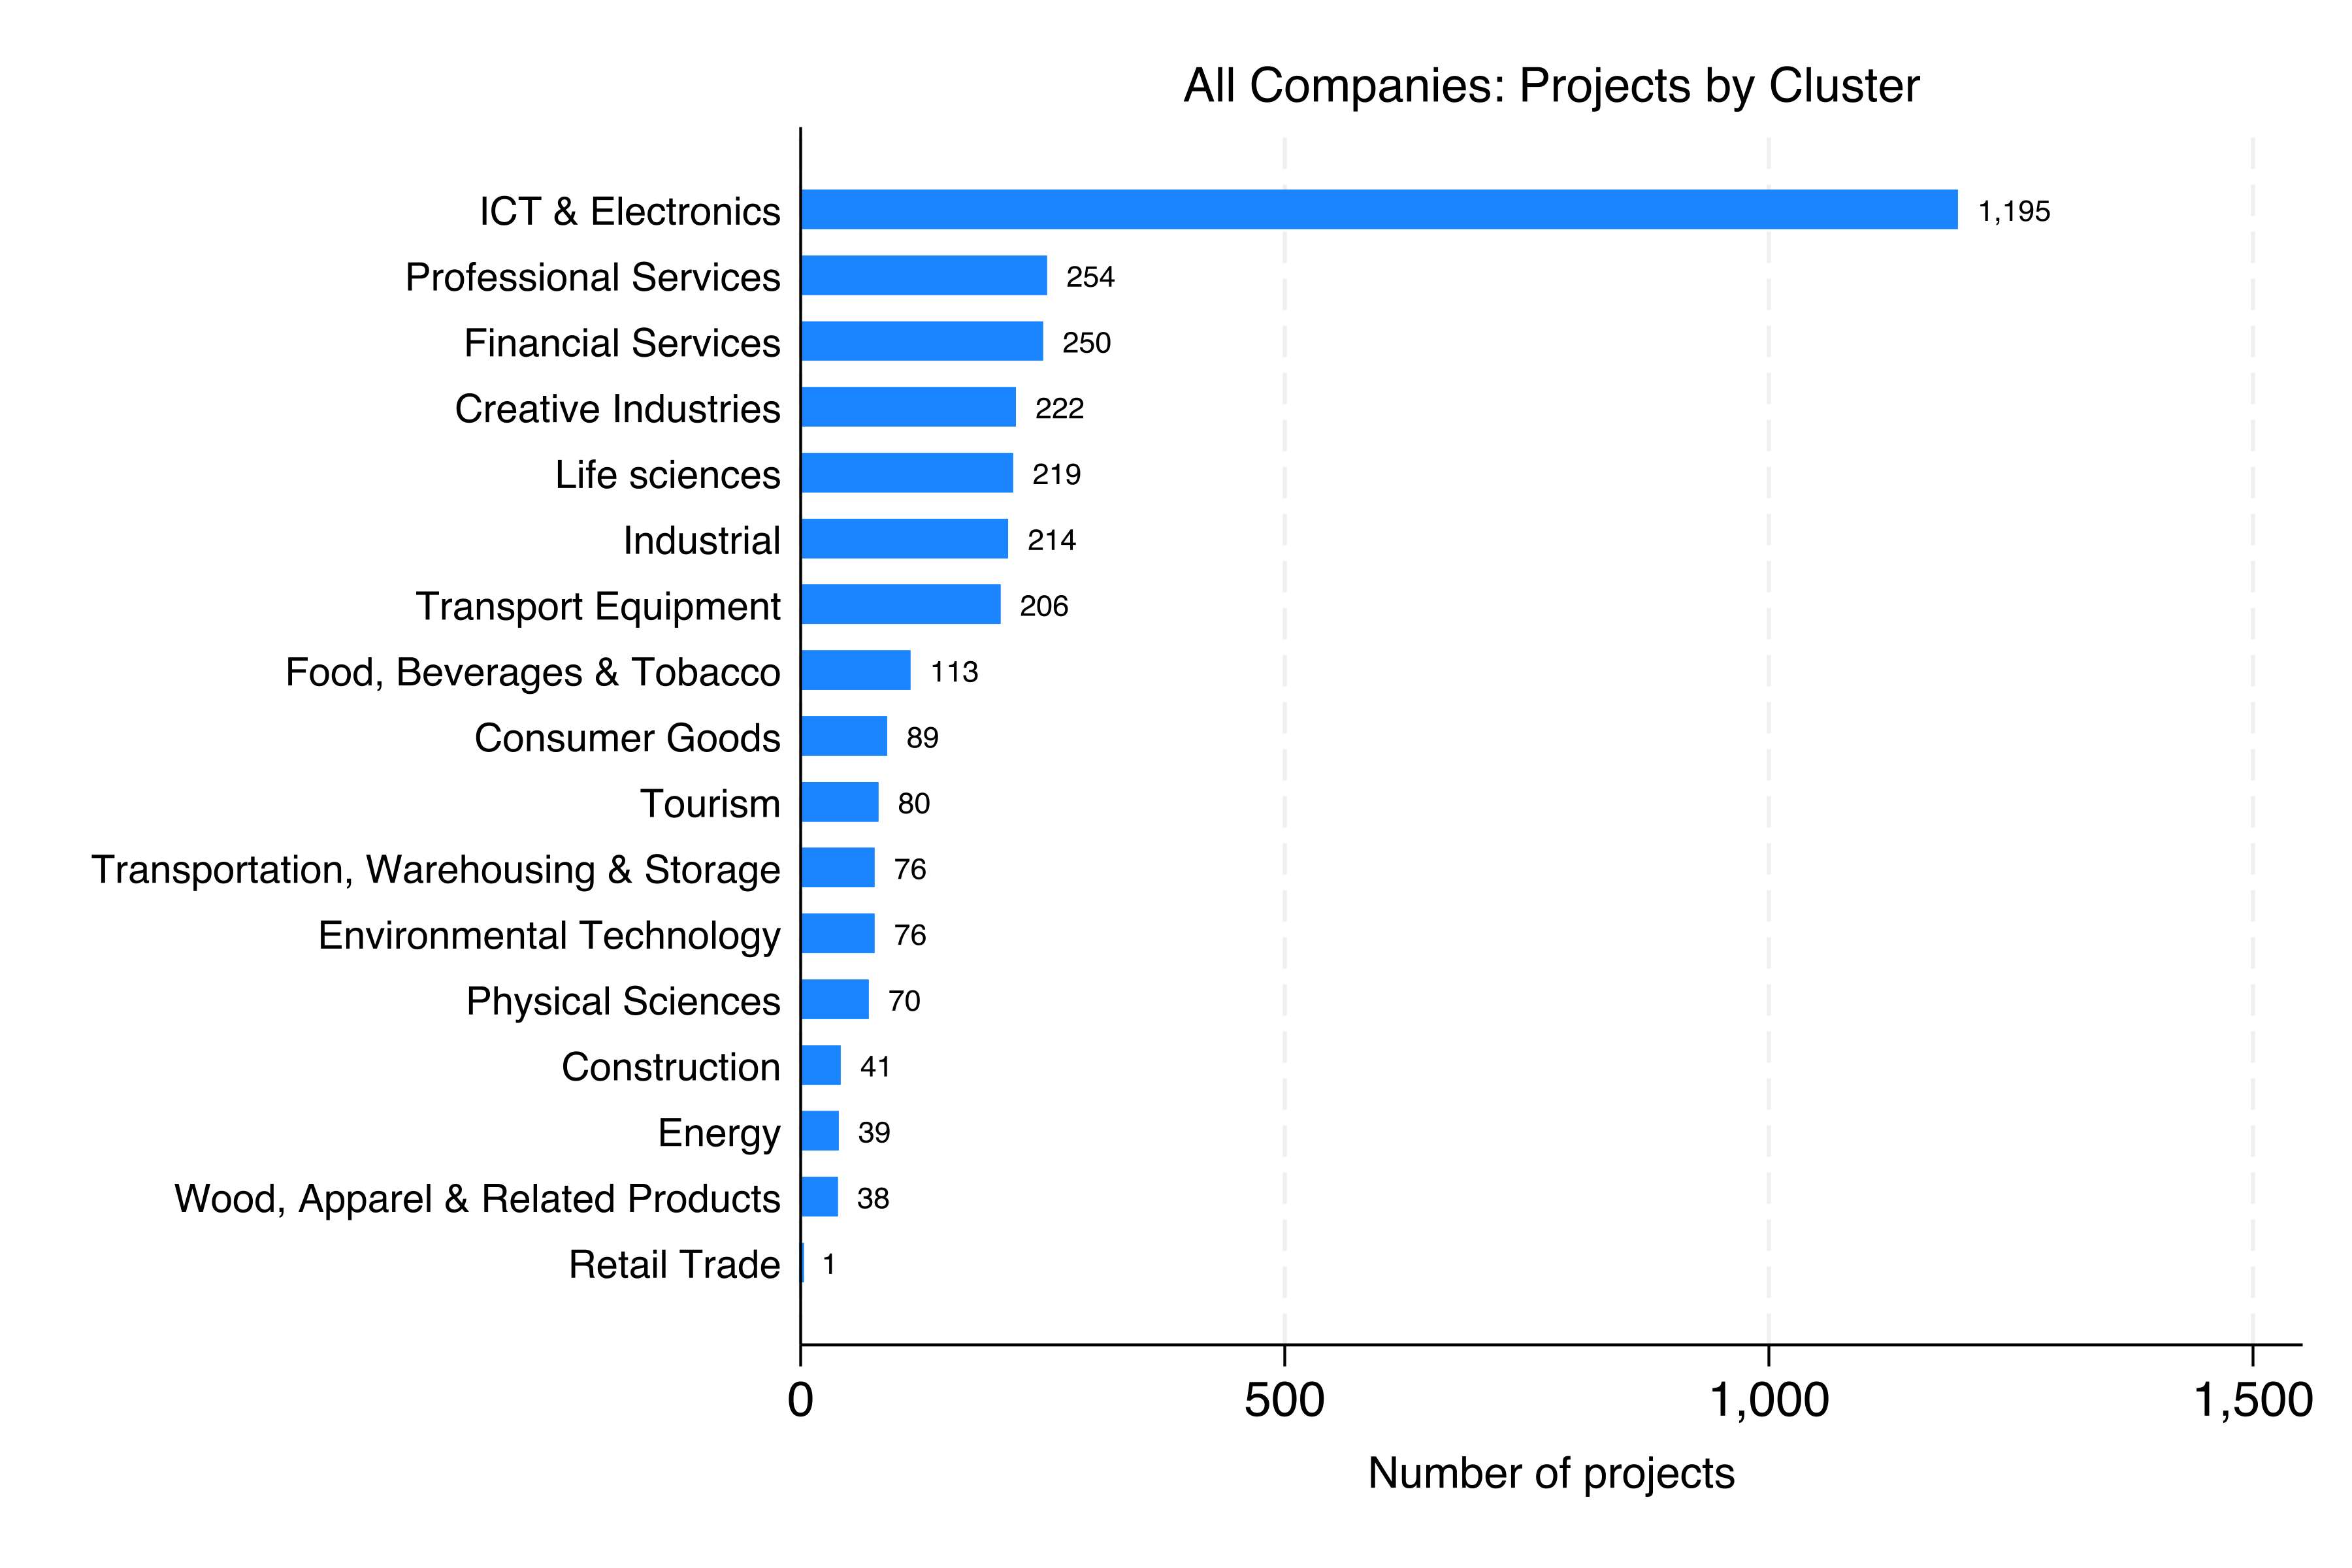
\includegraphics[width=1\linewidth]{4_5_figA22_projects_by_cluster.png}
    \caption{All companies by their sector (cluster)}
    \label{fig:all companies by sector}
\end{figure}

   As we conduct further investigation, we will deconstruct our samples further to get a more granular understanding of the behavior of our data.

\section{Additional Results} \label{sec:oa_results}

This section reports every result referenced but not shown in the paper. A caution applies to a few thin columns (Professional Services, Life Sciences, Industrial, Transport Equipment, Creative Industries, and Financial Services FDI, and the small-company tech-hub column): they have so few projects that PPML cannot really estimate them, which shows up as very large coefficients or standard errors of 0.000. Those cells should not be interpreted.

\subsection{FDI by Sector} \label{ss: sector}

\begin{table}[!htbp]
\centering
\scriptsize
\setlength{\tabcolsep}{2pt}
\renewcommand{\arraystretch}{1.08}
\caption{Sector cuts: category-level policy interactions}
\label{tab:final_cluster_table4_h3}
\begin{tabularx}{\textwidth}{@{}>{\RaggedRight\arraybackslash}X *{8}{>{\Centering\arraybackslash}X}@{}}
\hline
Specification & First-gen 25+ high-ed, all FDI & First-gen 25+ high-ed, ICT FDI & First-gen 25+ high-ed, Professional Services FDI & First-gen 25+ high-ed, Financial Services FDI & First-gen 25+ high-ed, Creative Industries FDI & First-gen 25+ high-ed, Life Sciences FDI & First-gen 25+ high-ed, Industrial FDI & First-gen 25+ high-ed, Transport Equipment FDI \\
\hline
Symbolic & 0.055 & 0.868*** & 8.700*** & 0.053*** & 0.150** & 0.000 & -10.224*** & -0.625 \\
 & (0.092) & (0.269) & (1.432) & (0.018) & (0.071) & (0.000) & (3.351) & (0.894) \\
State Bureaucracy & 0.015 & 0.135** &  & 0.011 & -0.012 & 0.000 & 0.000 & 0.000 \\
 & (0.016) & (0.057) &  & (0.021) & (0.019) & (0.000) & (0.000) & (0.000) \\
Abroad & -0.006 & 0.102 & -0.070 & 0.032 & 0.004*** & 0.000 & 0.000 & 0.000 \\
 & (0.024) & (0.081) & (0.044) & (0.026) & (0.001) & (0.000) & (0.000) & (0.000) \\
Info & -0.031*** & 0.151*** & 0.000 & -944.065 & 0.000 & 0.000 & 0.000 & 0.000 \\
 & (0.008) & (0.036) & (0.000) & (1345.299) & (0.000) & (0.000) & (0.000) & (0.000) \\
\hline
Raw sample N & 4897 & 4897 & 4897 & 4897 & 4897 & 4897 & 4897 & 4897 \\
Projects, 2005--2017 & 2130 & 791 & 187 & 255 & 158 & 109 & 145 & 113 \\
Total diaspora pop., 2005--2017 & 7021199 & 7021199 & 7021199 & 7021199 & 7021199 & 7021199 & 7021199 & 7021199 \\
e(N\_full) & 4897 & 4897 & 4897 & 4897 & 4897 & 4897 & 4897 & 4897 \\
e(N) & 1937 & 913 & 168-342 & 207 & 116-193 & 47-50 & 60-201 & 36-104 \\
Dropped singletons & 2960 & 3984 & 4555-4594 & 4690 & 4704-4730 & 4798-4806 & 4696-4760 & 4793-4826 \\
Dropped separated obs & 0 & 0 & 0-135 & 0 & 0-51 & 44-49 & 0-77 & 0-35 \\
\hline
\fulltablenote{9}{Cells are coefficients on ln\_dias or ln\_dias x policy, with SEs directly underneath.}
\fulltablenote{9}{* p<0.10, ** p<0.05, *** p<0.01.}
\end{tabularx}
\end{table}

\begin{table}[!htbp]
\centering
\scriptsize
\setlength{\tabcolsep}{2pt}
\renewcommand{\arraystretch}{1.08}
\caption{Sector cuts: single-policy interactions, 2+ states and more than 10 state-years}
\label{tab:final_cluster_appendix_singlepolicy}
\begin{tabularx}{\textwidth}{@{}>{\RaggedRight\arraybackslash}X *{10}{>{\Centering\arraybackslash}X}@{}}
\hline
Specification & \# States & \# State-years & First-gen 25+ high-ed, all FDI & First-gen 25+ high-ed, ICT FDI & First-gen 25+ high-ed, Professional Services FDI & First-gen 25+ high-ed, Financial Services FDI & First-gen 25+ high-ed, Creative Industries FDI & First-gen 25+ high-ed, Life Sciences FDI & First-gen 25+ high-ed, Industrial FDI & First-gen 25+ high-ed, Transport Equipment FDI \\
\hline
\multicolumn{11}{@{}>{\RaggedRight\arraybackslash}p{\dimexpr\linewidth-2\tabcolsep\relax}@{}}{\textit{Policies with 3+ states and 20+ state-years}}\\
Diaspora Admin Unit & 6 & 63 & 0.017 & 0.246*** & --- & 0.037 & 0.074*** & --- & --- & --- \\
 &  &  & (0.033) & (0.070) &  & (0.039) & (0.012) &  &  &  \\
Grievance Reporting & 4 & 39 & 0.030* & 0.160 & --- & -0.007 & 0.006*** & --- & --- & --- \\
 &  &  & (0.016) & (0.126) &  & (0.052) & (0.001) &  &  &  \\
Remains Repatriation & 3 & 34 & 0.020 & 0.104 & --- & 0.031 & -0.061 & --- & --- & --- \\
 &  &  & (0.024) & (0.108) &  & (0.057) & (0.050) &  &  &  \\
Manpower Companies & 3 & 33 & -0.021 & 0.129 & -0.069 & 0.040 & 0.006*** & --- & --- & --- \\
 &  &  & (0.036) & (0.087) & (0.096) & (0.059) & (0.001) &  &  &  \\
\multicolumn{11}{@{}>{\RaggedRight\arraybackslash}p{\dimexpr\linewidth-2\tabcolsep\relax}@{}}{\textit{Policies with 2+ states and more than 10 state-years}}\\
Tax \& Regulatory Guidance & 2 & 14 & -0.071*** & 0.298*** & --- & -1888.130 & --- & --- & --- & --- \\
 &  &  & (0.020) & (0.080) &  & (2690.597) &  &  &  &  \\
Investment Promotion Roadshows & 2 & 13 & -0.048** & 0.295*** & --- & -1888.130 & --- & --- & --- & --- \\
 &  &  & (0.019) & (0.054) &  & (2690.597) &  &  &  &  \\
\hline
Raw sample N &  &  & 4897 & 4897 & 4897 & 4897 & 4897 & 4897 & 4897 & 4897 \\
Projects, 2005--2017 &  &  & 2130 & 791 & 187 & 255 & 158 & 109 & 145 & 113 \\
Total diaspora pop., 2005--2017 &  &  & 7021199 & 7021199 & 7021199 & 7021199 & 7021199 & 7021199 & 7021199 & 7021199 \\
e(N\_full) &  &  & 4897 & 4897 & 4897 & 4897 & 4897 & 4897 & 4897 & 4897 \\
e(N) &  &  & 1937 & 899-913 & 168-342 & 207 & 116-193 & 43-50 & 60-201 & 36-104 \\
Dropped singletons &  &  & 2960 & 3984-3993 & 4555-4594 & 4690 & 4704-4730 & 4798-4806 & 4696-4760 & 4793-4826 \\
Dropped separated obs &  &  & 0 & 0-5 & 0-135 & 0 & 0-51 & 44-50 & 0-77 & 0-35 \\
\hline
\fulltablenote{11}{Cells are coefficients on ln\_dias x policy, with SEs clustered by Indian state directly underneath. All models include metro-state, metro-year, and state-year fixed effects. --- marks an interaction ppmlhdfe omits because it is not identified once singletons and separated observations are dropped.}
\fulltablenote{11}{* p<0.10, ** p<0.05, *** p<0.01.}
\end{tabularx}
\end{table}


The cluster cuts confirm that the main result is not evenly distributed across sectors. In the any-DEP model (Table~\pref{tab:final_cluster_table2_h1} in the paper), ICT is strongly positive and significant. Creative industries are also positive and significant, which is genuinely interesting and deserves future work. ICT, however, is the more convincing sector for deeper analysis because it has many more projects: 791 ICT projects, compared to 158 creative industries projects. That matters because once the model absorbs fixed effects and drops separated observations, small sectors can produce dramatic-looking coefficients identified off a very thin remaining slice of the data.

The category table (Table~\ref{tab:final_cluster_table4_h3}) reinforces the idea that all other industries are unstable. ICT has the most coherent pattern: symbolic, state bureaucracy, and information policies are all positive and significant. Creative industries also look promising, especially in the symbolic, state-bureaucracy, and abroad rows, but I treat that as suggestive rather than as a second main result. A warning sign emerges for further investigation of creative industries in that for many other sectors with the same size, coefficients are very unstable. We also see that the results for all industries are driven by freakishly large coefficients in certain sectors, so we can discount prior results that informational DEPs negatively influenced all-industry FDI.

The cluster section therefore points to ICT as the main sectoral story, with support from creative industries that the effectiveness of DEPs for ICT is driven by its position as a high-human-capital, low-startup-cost industry.

\FloatBarrier
\subsection{FDI by Activity} \label{ss:activity}

\begin{table}[!htbp]
\centering
\footnotesize
\setlength{\tabcolsep}{3pt}
\renewcommand{\arraystretch}{1.08}
\caption{Activity cuts: any DEP adoption x diaspora}
\label{tab:final_activity_table2_h1}
\begin{tabularx}{\textwidth}{@{}>{\RaggedRight\arraybackslash}X *{5}{>{\Centering\arraybackslash}X}@{}}
\hline
Specification & First-gen 25+ high-ed, all FDI & First-gen 25+ high-ed, Sales, Marketing \& Support FDI & First-gen 25+ high-ed, Design, Development \& Testing FDI & First-gen 25+ high-ed, Manufacturing FDI & First-gen 25+ high-ed, Business Services FDI \\
\hline
Any DEP adoption & -0.020 & 0.083 & 0.065 & -0.134 & -0.014 \\
 & (0.034) & (0.079) & (0.096) & (0.103) & (0.049) \\
\hline
Raw sample N & 4897 & 4897 & 4897 & 4897 & 4897 \\
Projects, 2005--2017 & 2130 & 520 & 533 & 271 & 313 \\
Total diaspora pop., 2005--2017 & 7021199 & 7021199 & 7021199 & 7021199 & 7021199 \\
e(N\_full) & 4897 & 4897 & 4897 & 4897 & 4897 \\
e(N) & 1937 & 929 & 759 & 488 & 351 \\
Dropped singletons & 2960 & 3968 & 4138 & 4409 & 4546 \\
Dropped separated obs & 0 & 0 & 0 & 0 & 0 \\
\hline
\fulltablenote{6}{Cells are coefficients on ln\_dias or ln\_dias x policy, with SEs directly underneath.}
\fulltablenote{6}{* p<0.10, ** p<0.05, *** p<0.01.}
\end{tabularx}
\end{table}

\begin{table}[!htbp]
\centering
\footnotesize
\setlength{\tabcolsep}{3pt}
\renewcommand{\arraystretch}{1.08}
\caption{Activity cuts: category-level policy interactions}
\label{tab:final_activity_table4_h3}
\begin{tabularx}{\textwidth}{@{}>{\RaggedRight\arraybackslash}X *{5}{>{\Centering\arraybackslash}X}@{}}
\hline
Specification & First-gen 25+ high-ed, all FDI & First-gen 25+ high-ed, Sales, Marketing \& Support FDI & First-gen 25+ high-ed, Design, Development \& Testing FDI & First-gen 25+ high-ed, Manufacturing FDI & First-gen 25+ high-ed, Business Services FDI \\
\hline
Symbolic & 0.055 & 0.193*** & 1.400*** & -0.395 & -0.543** \\
 & (0.092) & (0.070) & (0.500) & (0.326) & (0.251) \\
State Bureaucracy & 0.015 & 0.014 & 0.112*** & 0.033 & 0.020 \\
 & (0.016) & (0.038) & (0.037) & (0.066) & (0.017) \\
Abroad & -0.006 & -0.018 & 0.064 & 0.019 & 0.012 \\
 & (0.024) & (0.062) & (0.078) & (0.056) & (0.019) \\
Info & -0.031*** & -0.017 & -0.061*** & -0.021 & -0.563 \\
 & (0.008) & (0.041) & (0.022) & (0.024) & (0.347) \\
\hline
Raw sample N & 4897 & 4897 & 4897 & 4897 & 4897 \\
Projects, 2005--2017 & 2130 & 520 & 533 & 271 & 313 \\
Total diaspora pop., 2005--2017 & 7021199 & 7021199 & 7021199 & 7021199 & 7021199 \\
e(N\_full) & 4897 & 4897 & 4897 & 4897 & 4897 \\
e(N) & 1937 & 929 & 759 & 488 & 351 \\
Dropped singletons & 2960 & 3968 & 4138 & 4409 & 4546 \\
Dropped separated obs & 0 & 0 & 0 & 0 & 0 \\
\hline
\fulltablenote{6}{Cells are coefficients on ln\_dias x policy, with SEs clustered by Indian state directly underneath. All models include metro-state, metro-year, and state-year fixed effects. --- marks an interaction ppmlhdfe omits because it is not identified once singletons and separated observations are dropped.}
\fulltablenote{6}{* p<0.10, ** p<0.05, *** p<0.01.}
\end{tabularx}
\end{table}

\begin{table}[!htbp]
\centering
\scriptsize
\setlength{\tabcolsep}{2pt}
\renewcommand{\arraystretch}{1.08}
\caption{Activity cuts: single-policy interactions, 2+ states and more than 10 state-years}
\label{tab:final_activity_appendix_singlepolicy}
\begin{tabularx}{\textwidth}{@{}>{\RaggedRight\arraybackslash}X *{7}{>{\Centering\arraybackslash}X}@{}}
\hline
Specification & \# States & \# State-years & First-gen 25+ high-ed, all FDI & First-gen 25+ high-ed, Sales, Marketing \& Support FDI & First-gen 25+ high-ed, Design, Development \& Testing FDI & First-gen 25+ high-ed, Manufacturing FDI & First-gen 25+ high-ed, Business Services FDI \\
\hline
\multicolumn{8}{@{}>{\RaggedRight\arraybackslash}p{\dimexpr\linewidth-2\tabcolsep\relax}@{}}{\textit{Policies with 3+ states and 20+ state-years}}\\
Diaspora Admin Unit & 6 & 63 & 0.017 & 0.037 & 0.159** & 0.027 & 0.026 \\
 &  &  & (0.033) & (0.054) & (0.070) & (0.114) & (0.034) \\
Grievance Reporting & 4 & 39 & 0.030* & -0.004 & 0.173*** & 0.064 & 0.044 \\
 &  &  & (0.016) & (0.101) & (0.050) & (0.106) & (0.029) \\
Remains Repatriation & 3 & 34 & 0.020 & -0.165 & 0.258*** & 0.251* & 0.060 \\
 &  &  & (0.024) & (0.122) & (0.091) & (0.141) & (0.065) \\
Manpower Companies & 3 & 33 & -0.021 & 0.053 & 0.019 & -0.077** & -0.005 \\
 &  &  & (0.036) & (0.068) & (0.074) & (0.033) & (0.027) \\
\multicolumn{8}{@{}>{\RaggedRight\arraybackslash}p{\dimexpr\linewidth-2\tabcolsep\relax}@{}}{\textit{Policies with 2+ states and more than 10 state-years}}\\
Tax \& Regulatory Guidance & 2 & 14 & -0.071*** & -0.066 & -0.118*** & -0.049 & -0.499 \\
 &  &  & (0.020) & (0.098) & (0.044) & (0.048) & (0.326) \\
Investment Promotion Roadshows & 2 & 13 & -0.048** & 0.006 & -0.124*** & -0.035 & -687.544*** \\
 &  &  & (0.019) & (0.057) & (0.045) & (0.049) & (7.736) \\
\hline
Raw sample N &  &  & 4897 & 4897 & 4897 & 4897 & 4897 \\
Projects, 2005--2017 &  &  & 2130 & 520 & 533 & 271 & 313 \\
Total diaspora pop., 2005--2017 &  &  & 7021199 & 7021199 & 7021199 & 7021199 & 7021199 \\
e(N\_full) &  &  & 4897 & 4897 & 4897 & 4897 & 4897 \\
e(N) &  &  & 1937 & 929 & 759 & 488 & 351 \\
Dropped singletons &  &  & 2960 & 3968 & 4138 & 4409 & 4546 \\
Dropped separated obs &  &  & 0 & 0 & 0 & 0 & 0 \\
\hline
\fulltablenote{8}{Cells are coefficients on ln\_dias x policy, with SEs clustered by Indian state directly underneath. All models include metro-state, metro-year, and state-year fixed effects. --- marks an interaction ppmlhdfe omits because it is not identified once singletons and separated observations are dropped.}
\fulltablenote{8}{* p<0.10, ** p<0.05, *** p<0.01.}
\end{tabularx}
\end{table}


The activity cuts are weaker than the cluster cuts, which is useful in itself. In the any-DEP model (Table~\ref{tab:final_activity_table2_h1}), none of the activity-specific any-DEP coefficients are statistically significant. That means the ICT result is not simply reducible to one broad project activity like sales, design, manufacturing, or business services. Put differently, it is not just that DEPs help sales offices or design projects wherever they appear. The sectoral identity of ICT seems to matter more than these broad activity classifications. The category table (Table~\ref{tab:final_activity_table4_h3}) is messier. Symbolic policies are positive for sales and design activity, and state-bureaucratic policies are positive for design. However, business services has a large negative symbolic coefficient, and the single-policy shows an especially extreme negative estimate for investment promotion roadshows. I do not give that business-services result a clean substantive interpretation. It is better read as a sign of heterogeneity and instability in a smaller effective sample, not as a neat theory of why roadshows would reduce business services FDI. The honest takeaway is that the any-DEP model gives us no significant activity-level result, while the category table has some interesting but not yet clean heterogeneity.

\FloatBarrier
\subsection{FDI by Company Size} \label{ss:comp size}
\begin{table}[!htbp]
\centering
\footnotesize
\setlength{\tabcolsep}{3pt}
\renewcommand{\arraystretch}{1.08}
\caption{H0: location-specific diaspora versus national Indian diaspora stock: company-size FDI samples}
\label{tab:final_company_size_h0}
\begin{tabularx}{\textwidth}{@{}>{\RaggedRight\arraybackslash}X *{4}{>{\Centering\arraybackslash}X}@{}}
\hline
Specification & First-gen 25+ high-ed, all FDI, small-75 companies & First-gen 25+ high-ed, ICT FDI, small-75 companies & First-gen 25+ high-ed, all FDI, large-75 companies & First-gen 25+ high-ed, ICT FDI, large-75 companies \\
\hline
Subnational diaspora: exporter FE + importer-year FE & 0.006 & 0.030 & 0.093** & 0.095 \\
 & (0.048) & (0.094) & (0.040) & (0.058) \\
National Indian diaspora: exporter FE + importer-year FE & -0.785* & -0.184 & 0.026 & 0.147 \\
 & (0.411) & (0.662) & (0.238) & (0.352) \\
\hline
Raw sample N & 4897 & 4897 & 4897 & 4897 \\
Projects, 2005--2017 & 585 & 241 & 1545 & 550 \\
Total diaspora pop., 2005--2017 & 7021199 & 7021199 & 7021199 & 7021199 \\
e(N\_full) & 4897 & 4897 & 4897 & 4897 \\
e(N) & 2603 & 1636 & 3338 & 2020 \\
Dropped singletons & 2294 & 3261 & 1559 & 2877 \\
Dropped separated obs & 0 & 0 & 0 & 0 \\
\hline
\fulltablenote{5}{Cells are coefficients on ln\_dias (or the national Indian diaspora), with SEs clustered by metro-state pair directly underneath. Fixed effects as listed in each row.}
\fulltablenote{5}{* p<0.10, ** p<0.05, *** p<0.01.}
\end{tabularx}
\end{table}


Table~\ref{tab:final_company_size_h0} shows that the company-size split makes the descriptive $H_0$ relationship more demanding, but not damaging to the overall argument. Among small-company projects, the subnational diaspora coefficients are positive but not statistically significant for both all FDI and ICT FDI. This is weaker than the large-company all-FDI result, but it is still substantively preferable to the national-diaspora comparison: national Indian diaspora stock is negative for small-company FDI and even marginally significant in the all-FDI small-company sample. Thus, even in the thinner small-company sample, the subnational measure does not produce the negative relationship that appears for national diaspora size. This supports the broader claim that location-specific diaspora measurement is still more appropriate than national diaspora stock, even when the project sample is restricted to smaller firms.

\begin{table}[!htbp]
\centering
\footnotesize
\setlength{\tabcolsep}{3pt}
\renewcommand{\arraystretch}{1.08}
\caption{Diaspora-only PPML: company-size FDI samples}
\label{tab:final_company_size_table1_baseline}
\begin{tabularx}{\textwidth}{@{}>{\RaggedRight\arraybackslash}X *{4}{>{\Centering\arraybackslash}X}@{}}
\hline
Specification & First-gen 25+ high-ed, all FDI, small-75 companies & First-gen 25+ high-ed, ICT FDI, small-75 companies & First-gen 25+ high-ed, all FDI, large-75 companies & First-gen 25+ high-ed, ICT FDI, large-75 companies \\
\hline
PPML exporter-year FE + importer-year FE & -0.010 & -0.010 & 0.068** & 0.009 \\
 & (0.044) & (0.076) & (0.032) & (0.048) \\
PPML exporter FE + importer-year FE & 0.006 & 0.030 & 0.093** & 0.095 \\
 & (0.048) & (0.094) & (0.040) & (0.058) \\
\hline
Raw sample N & 4897 & 4897 & 4897 & 4897 \\
Projects, 2005--2017 & 585 & 241 & 1545 & 550 \\
Total diaspora pop., 2005--2017 & 7021199 & 7021199 & 7021199 & 7021199 \\
e(N\_full) & 4897 & 4897 & 4897 & 4897 \\
e(N) & 1268-2603 & 595-1636 & 2141-3338 & 948-2020 \\
Dropped singletons & 2294-3629 & 3261-4302 & 1559-2756 & 2877-3949 \\
Dropped separated obs & 0 & 0 & 0 & 0 \\
\hline
\fulltablenote{5}{Cells are coefficients on ln\_dias or ln\_dias x policy, with SEs directly underneath.}
\fulltablenote{5}{* p<0.10, ** p<0.05, *** p<0.01.}
\end{tabularx}
\end{table}


Table~\ref{tab:final_company_size_table1_baseline} reinforces the same interpretation. The unconditional diaspora--FDI slope is not consistently positive for small-company FDI once the model includes more demanding fixed effects. However, this should not be overread as evidence that small firms are unrelated to diasporas. These samples contain far fewer projects, especially in the small-company ICT column, and the fixed effects absorb much of the remaining variation. More importantly, the baseline table only asks whether diaspora size alone predicts project counts; the more theoretically relevant question is whether diaspora engagement policies change how diaspora size translates into FDI.
\begin{table}[!htbp]
\centering
\footnotesize
\setlength{\tabcolsep}{3pt}
\renewcommand{\arraystretch}{1.08}
\caption{DEP-count intensity x diaspora: company-size FDI samples}
\label{tab:final_company_size_table3_h2}
\begin{tabularx}{\textwidth}{@{}>{\RaggedRight\arraybackslash}X *{4}{>{\Centering\arraybackslash}X}@{}}
\hline
Specification & First-gen 25+ high-ed, all FDI, small-75 companies & First-gen 25+ high-ed, ICT FDI, small-75 companies & First-gen 25+ high-ed, all FDI, large-75 companies & First-gen 25+ high-ed, ICT FDI, large-75 companies \\
\hline
DEP count (support-screened) & -0.008 & 0.000 & 0.002 & 0.113*** \\
 & (0.031) & (0.086) & (0.020) & (0.043) \\
\hline
Raw sample N & 4897 & 4897 & 4897 & 4897 \\
Projects, 2005--2017 & 585 & 241 & 1545 & 550 \\
Total diaspora pop., 2005--2017 & 7021199 & 7021199 & 7021199 & 7021199 \\
e(N\_full) & 4897 & 4897 & 4897 & 4897 \\
e(N) & 885 & 367 & 1663 & 673 \\
Dropped singletons & 4012 & 4530 & 3234 & 4224 \\
Dropped separated obs & 0 & 0 & 0 & 0 \\
\hline
\fulltablenote{5}{Cells are coefficients on ln\_dias or ln\_dias x policy, with SEs directly underneath.}
\fulltablenote{5}{* p<0.10, ** p<0.05, *** p<0.01.}
\end{tabularx}
\end{table}


Table~\ref{tab:final_company_size_table3_h2} shows that the company-size split weakens the $H_2$ count-intensity result for smaller firms. The DEP-count interaction is essentially zero for small-company ICT FDI, while it is positive and significant for large-company ICT FDI. This suggests that, for smaller firms, the number of DEP categories adopted may matter less than the presence of the right kind of policy. That interpretation is substantively reasonable: a small diaspora-linked firm is unlikely to benefit simply because a state has accumulated many diaspora-facing programs, especially if some are symbolic, bureaucratic, or welfare-oriented. Instead, small firms should benefit most from policies that directly reduce the information and procedural costs of investing.

The paper shows the company-size Tables 2 and 4 and the single-policy table (Tables~\pref{tab:final_company_size_table2_h1}, \pref{tab:final_company_size_table4_h3}, and \pref{tab:final_company_size_appendix_singlepolicy}).

\FloatBarrier
\subsection{A Deeper Look at ICT} \label{ss:ict}

The paper shows the any-DEP results across diaspora definitions and the ICT-worker category results (Tables~\pref{tab:final_ict_generations_education_table2_h1} and \pref{tab:final_ict_worker_table4_h3}). The remaining ICT tables follow.

\begin{table}[!htbp]
\centering
\footnotesize
\setlength{\tabcolsep}{3pt}
\renewcommand{\arraystretch}{1.08}
\caption{ICT FDI by diaspora generation and education: category-level policy interactions}
\label{tab:final_ict_generations_education_table4_h3}
\begin{tabularx}{\textwidth}{@{}>{\RaggedRight\arraybackslash}X *{4}{>{\Centering\arraybackslash}X}@{}}
\hline
Specification & First-gen 25+ all diaspora, ICT FDI & All-gen 25+ all diaspora, ICT FDI & First-gen 25+ high-ed, ICT FDI & All-gen 25+ high-ed, ICT FDI \\
\hline
Symbolic & 0.764*** & 0.698*** & 0.868*** & 0.786*** \\
 & (0.258) & (0.244) & (0.269) & (0.248) \\
State Bureaucracy & 0.118** & 0.128** & 0.135** & 0.146** \\
 & (0.059) & (0.063) & (0.057) & (0.063) \\
Abroad & 0.074 & 0.092 & 0.102 & 0.112 \\
 & (0.075) & (0.089) & (0.081) & (0.097) \\
Info & 0.199*** & 0.337*** & 0.151*** & 0.169*** \\
 & (0.041) & (0.073) & (0.036) & (0.042) \\
\hline
Raw sample N & 5025 & 4546 & 4897 & 4437 \\
Projects, 2005--2017 & 791 & 772 & 791 & 772 \\
Total diaspora pop., 2005--2017 & 9867596 & 10785954 & 7021199 & 7462214 \\
e(N\_full) & 5025 & 4546 & 4897 & 4437 \\
e(N) & 915 & 848 & 913 & 845 \\
Dropped singletons & 4110 & 3698 & 3984 & 3592 \\
Dropped separated obs & 0 & 0 & 0 & 0 \\
\hline
\fulltablenote{5}{Cells are coefficients on ln\_dias or ln\_dias x policy, with SEs directly underneath.}
\fulltablenote{5}{* p<0.10, ** p<0.05, *** p<0.01.}
\end{tabularx}
\end{table}

\begin{table}[!htbp]
\centering
\footnotesize
\setlength{\tabcolsep}{3pt}
\renewcommand{\arraystretch}{1.08}
\caption{ICT FDI by diaspora generation and education: single-policy interactions, 2+ states and more than 10 state-years}
\label{tab:final_ict_generations_education_appendix_singlepolicy}
\begin{tabularx}{\textwidth}{@{}>{\RaggedRight\arraybackslash}X *{6}{>{\Centering\arraybackslash}X}@{}}
\hline
Specification & \# States & \# State-years & First-gen 25+ all diaspora, ICT FDI & All-gen 25+ all diaspora, ICT FDI & First-gen 25+ high-ed, ICT FDI & All-gen 25+ high-ed, ICT FDI \\
\hline
\multicolumn{7}{@{}>{\RaggedRight\arraybackslash}p{\dimexpr\linewidth-2\tabcolsep\relax}@{}}{\textit{Policies with 3+ states and 20+ state-years}}\\
Diaspora Admin Unit & 6 & 63 & 0.221*** & 0.238*** & 0.246*** & 0.267*** \\
 &  &  & (0.076) & (0.083) & (0.070) & (0.075) \\
Grievance Reporting & 4 & 39 & 0.129 & 0.144 & 0.160 & 0.165 \\
 &  &  & (0.120) & (0.131) & (0.126) & (0.139) \\
Remains Repatriation & 3 & 34 & 0.083 & 0.101 & 0.104 & 0.126 \\
 &  &  & (0.112) & (0.123) & (0.108) & (0.130) \\
Manpower Companies & 3 & 33 & 0.090 & 0.111 & 0.129 & 0.133 \\
 &  &  & (0.079) & (0.093) & (0.087) & (0.103) \\
\multicolumn{7}{@{}>{\RaggedRight\arraybackslash}p{\dimexpr\linewidth-2\tabcolsep\relax}@{}}{\textit{Policies with 2+ states and more than 10 state-years}}\\
Tax \& Regulatory Guidance & 2 & 14 & 0.393*** & 0.672*** & 0.298*** & 0.348*** \\
 &  &  & (0.087) & (0.145) & (0.080) & (0.097) \\
Investment Promotion Roadshows & 2 & 13 & 0.384*** & 0.637*** & 0.295*** & 0.315*** \\
 &  &  & (0.059) & (0.094) & (0.054) & (0.056) \\
\hline
Raw sample N &  &  & 5025 & 4546 & 4897 & 4437 \\
Projects, 2005--2017 &  &  & 791 & 772 & 791 & 772 \\
Total diaspora pop., 2005--2017 &  &  & 9867596 & 10785954 & 7021199 & 7462214 \\
e(N\_full) &  &  & 5025 & 4546 & 4897 & 4437 \\
e(N) &  &  & 915 & 848 & 899-913 & 845 \\
Dropped singletons &  &  & 4110 & 3698 & 3984-3993 & 3592 \\
Dropped separated obs &  &  & 0 & 0 & 0-5 & 0 \\
\hline
\fulltablenote{7}{Cells are coefficients on ln\_dias x policy, with SEs clustered by Indian state directly underneath. All models include metro-state, metro-year, and state-year fixed effects. --- marks an interaction ppmlhdfe omits because it is not identified once singletons and separated observations are dropped.}
\fulltablenote{7}{* p<0.10, ** p<0.05, *** p<0.01.}
\end{tabularx}
\end{table}

\begin{table}[!htbp]
\centering
\footnotesize
\setlength{\tabcolsep}{3pt}
\renewcommand{\arraystretch}{1.08}
\caption{ICT FDI, ICT-worker diaspora: any DEP adoption x diaspora}
\label{tab:final_ict_worker_table2_h1}
\begin{tabularx}{\textwidth}{@{}>{\RaggedRight\arraybackslash}X *{4}{>{\Centering\arraybackslash}X}@{}}
\hline
Specification & First-gen 25+ high-ed, ICT FDI & All-gen 25+ high-ed, ICT FDI & First-gen 25+ high-ed, ICT FDI, ICT worker & All-gen 25+ high-ed, ICT FDI, ICT worker \\
\hline
Any DEP adoption & 0.242*** & 0.267*** & 0.232*** & 0.254*** \\
 & (0.045) & (0.041) & (0.054) & (0.062) \\
\hline
Raw sample N & 4897 & 4437 & 3490 & 3217 \\
Projects, 2005--2017 & 791 & 772 & 721 & 710 \\
Total diaspora pop., 2005--2017 & 7021199 & 7462214 & 2033705 & 2032626 \\
e(N\_full) & 4897 & 4437 & 3490 & 3217 \\
e(N) & 913 & 845 & 772 & 724 \\
Dropped singletons & 3984 & 3592 & 2718 & 2493 \\
Dropped separated obs & 0 & 0 & 0 & 0 \\
\hline
\fulltablenote{5}{Cells are coefficients on ln\_dias x policy, with SEs clustered by Indian state directly underneath. All models include metro-state, metro-year, and state-year fixed effects. --- marks an interaction ppmlhdfe omits because it is not identified once singletons and separated observations are dropped.}
\fulltablenote{5}{* p<0.10, ** p<0.05, *** p<0.01.}
\end{tabularx}
\end{table}

\begin{table}[!htbp]
\centering
\footnotesize
\setlength{\tabcolsep}{3pt}
\renewcommand{\arraystretch}{1.08}
\caption{ICT FDI, ICT-worker diaspora: single-policy interactions, 2+ states and more than 10 state-years}
\label{tab:final_ict_worker_appendix_singlepolicy}
\begin{tabularx}{\textwidth}{@{}>{\RaggedRight\arraybackslash}X *{6}{>{\Centering\arraybackslash}X}@{}}
\hline
Specification & \# States & \# State-years & First-gen 25+ high-ed, ICT FDI & All-gen 25+ high-ed, ICT FDI & First-gen 25+ high-ed, ICT FDI, ICT worker & All-gen 25+ high-ed, ICT FDI, ICT worker \\
\hline
\multicolumn{7}{@{}>{\RaggedRight\arraybackslash}p{\dimexpr\linewidth-2\tabcolsep\relax}@{}}{\textit{Policies with 3+ states and 20+ state-years}}\\
Diaspora Admin Unit & 6 & 63 & 0.246*** & 0.267*** & 0.233*** & 0.247*** \\
 &  &  & (0.070) & (0.075) & (0.071) & (0.085) \\
Grievance Reporting & 4 & 39 & 0.160 & 0.165 & 0.129 & 0.135 \\
 &  &  & (0.126) & (0.139) & (0.144) & (0.168) \\
Remains Repatriation & 3 & 34 & 0.104 & 0.126 & 0.089 & 0.117 \\
 &  &  & (0.108) & (0.130) & (0.166) & (0.212) \\
Manpower Companies & 3 & 33 & 0.129 & 0.133 & 0.115 & 0.128 \\
 &  &  & (0.087) & (0.103) & (0.098) & (0.115) \\
\multicolumn{7}{@{}>{\RaggedRight\arraybackslash}p{\dimexpr\linewidth-2\tabcolsep\relax}@{}}{\textit{Policies with 2+ states and more than 10 state-years}}\\
Tax Regulatory Guidance & 2 & 14 & 0.298*** & 0.348*** & -0.873*** & -0.681*** \\
 &  &  & (0.080) & (0.097) & (0.221) & (0.181) \\
Investment Promotion Roadshows & 2 & 13 & 0.295*** & 0.315*** & -0.684*** & -0.540*** \\
 &  &  & (0.054) & (0.056) & (0.178) & (0.120) \\
\hline
Raw sample N &  &  & 4897 & 4437 & 3490 & 3217 \\
Projects, 2005--2017 &  &  & 791 & 772 & 721 & 710 \\
Total diaspora pop., 2005--2017 &  &  & 7021199 & 7462214 & 2033705 & 2032626 \\
e(N\_full) &  &  & 4897 & 4437 & 3490 & 3217 \\
e(N) &  &  & 899-913 & 845 & 772 & 724 \\
Dropped singletons &  &  & 3984-3993 & 3592 & 2718 & 2493 \\
Dropped separated obs &  &  & 0-5 & 0 & 0 & 0 \\
\hline
\fulltablenote{7}{Cells are coefficients on ln\_dias or ln\_dias x policy, with SEs directly underneath.}
\fulltablenote{7}{* p<0.10, ** p<0.05, *** p<0.01.}
\end{tabularx}
\end{table}

\begin{table}[!htbp]
\centering
\footnotesize
\setlength{\tabcolsep}{3pt}
\renewcommand{\arraystretch}{1.08}
\caption{ICT FDI by company size: any DEP adoption x diaspora}
\label{tab:final_ict_company_size_table2_h1}
\begin{tabularx}{\textwidth}{@{}>{\RaggedRight\arraybackslash}X *{4}{>{\Centering\arraybackslash}X}@{}}
\hline
Specification & First-gen 25+ high-ed, ICT FDI, all companies & First-gen 25+ high-ed, ICT FDI, all companies, ICT worker & First-gen 25+ high-ed, ICT FDI, small-75 companies & First-gen 25+ high-ed, ICT FDI, small-75 companies, ICT worker \\
\hline
Any DEP adoption & 0.242*** & 0.232*** & 0.212** & 0.216 \\
 & (0.045) & (0.054) & (0.103) & (0.152) \\
\hline
Raw sample N & 4897 & 3490 & 4897 & 3490 \\
Projects, 2005--2017 & 791 & 721 & 241 & 214 \\
Total diaspora pop., 2005--2017 & 7021199 & 2033705 & 7021199 & 2033705 \\
e(N\_full) & 4897 & 3490 & 4897 & 3490 \\
e(N) & 913 & 772 & 367 & 288 \\
Dropped singletons & 3984 & 2718 & 4530 & 3202 \\
Dropped separated obs & 0 & 0 & 0 & 0 \\
\hline
\fulltablenote{5}{Cells are coefficients on ln\_dias x policy, with SEs clustered by Indian state directly underneath. All models include metro-state, metro-year, and state-year fixed effects. --- marks an interaction ppmlhdfe omits because it is not identified once singletons and separated observations are dropped.}
\fulltablenote{5}{* p<0.10, ** p<0.05, *** p<0.01.}
\end{tabularx}
\end{table}

\begin{table}[!htbp]
\centering
\footnotesize
\setlength{\tabcolsep}{3pt}
\renewcommand{\arraystretch}{1.08}
\caption{ICT FDI by company size: category-level policy interactions}
\label{tab:final_ict_company_size_table4_h3}
\begin{tabularx}{\textwidth}{@{}>{\RaggedRight\arraybackslash}X *{4}{>{\Centering\arraybackslash}X}@{}}
\hline
Specification & First-gen 25+ high-ed, ICT FDI, all companies & First-gen 25+ high-ed, ICT FDI, all companies, ICT worker & First-gen 25+ high-ed, ICT FDI, small-75 companies & First-gen 25+ high-ed, ICT FDI, small-75 companies, ICT worker \\
\hline
Symbolic & 0.868*** & 1.217*** & 1.967 & 1.902* \\
 & (0.269) & (0.253) & (1.285) & (1.038) \\
State Bureaucracy & 0.135** & 0.120** & -0.064 & -0.098 \\
 & (0.057) & (0.061) & (0.141) & (0.122) \\
Abroad & 0.102 & 0.088 & -0.133 & -0.259 \\
 & (0.081) & (0.084) & (0.212) & (0.243) \\
Info & 0.151*** & -0.432*** & 0.093*** & -0.323*** \\
 & (0.036) & (0.149) & (0.027) & (0.090) \\
\hline
Raw sample N & 4897 & 3490 & 4897 & 3490 \\
Projects, 2005--2017 & 791 & 721 & 241 & 214 \\
Total diaspora pop., 2005--2017 & 7021199 & 2033705 & 7021199 & 2033705 \\
e(N\_full) & 4897 & 3490 & 4897 & 3490 \\
e(N) & 913 & 772 & 367 & 288 \\
Dropped singletons & 3984 & 2718 & 4530 & 3202 \\
Dropped separated obs & 0 & 0 & 0 & 0 \\
\hline
\fulltablenote{5}{Cells are coefficients on ln\_dias x policy, with SEs clustered by Indian state directly underneath. All models include metro-state, metro-year, and state-year fixed effects. --- marks an interaction ppmlhdfe omits because it is not identified once singletons and separated observations are dropped.}
\fulltablenote{5}{* p<0.10, ** p<0.05, *** p<0.01.}
\end{tabularx}
\end{table}

\begin{table}[!htbp]
\centering
\footnotesize
\setlength{\tabcolsep}{3pt}
\renewcommand{\arraystretch}{1.08}
\caption{ICT FDI by company size: single-policy interactions, 2+ states and more than 10 state-years}
\label{tab:final_ict_company_size_appendix_singlepolicy}
\begin{tabularx}{\textwidth}{@{}>{\RaggedRight\arraybackslash}X *{6}{>{\Centering\arraybackslash}X}@{}}
\hline
Specification & \# States & \# State-years & First-gen 25+ high-ed, ICT FDI, all companies & First-gen 25+ high-ed, ICT FDI, all companies, ICT worker & First-gen 25+ high-ed, ICT FDI, small-75 companies & First-gen 25+ high-ed, ICT FDI, small-75 companies, ICT worker \\
\hline
\multicolumn{7}{@{}>{\RaggedRight\arraybackslash}p{\dimexpr\linewidth-2\tabcolsep\relax}@{}}{\textit{Policies with 3+ states and 20+ state-years}}\\
Diaspora Admin Unit & 6 & 63 & 0.246*** & 0.233*** & 0.104 & 0.156 \\
 &  &  & (0.070) & (0.071) & (0.188) & (0.221) \\
Grievance Reporting & 4 & 39 & 0.160 & 0.129 & -0.310 & -0.470** \\
 &  &  & (0.126) & (0.144) & (0.224) & (0.223) \\
Remains Repatriation & 3 & 34 & 0.104 & 0.089 & 0.257 & 0.830 \\
 &  &  & (0.108) & (0.166) & (0.326) & (0.510) \\
Manpower Companies & 3 & 33 & 0.129 & 0.115 & -0.244 & -0.478* \\
 &  &  & (0.087) & (0.098) & (0.209) & (0.245) \\
\multicolumn{7}{@{}>{\RaggedRight\arraybackslash}p{\dimexpr\linewidth-2\tabcolsep\relax}@{}}{\textit{Policies with 2+ states and more than 10 state-years}}\\
Tax \& Regulatory Guidance & 2 & 14 & 0.298*** & -0.873*** & 0.174** & -0.646*** \\
 &  &  & (0.080) & (0.221) & (0.069) & (0.180) \\
Investment Promotion Roadshows & 2 & 13 & 0.295*** & -0.684*** & 0.194*** & -0.646*** \\
 &  &  & (0.054) & (0.178) & (0.039) & (0.180) \\
\hline
Raw sample N &  &  & 4897 & 3490 & 4897 & 3490 \\
Projects, 2005--2017 &  &  & 791 & 721 & 241 & 214 \\
Total diaspora pop., 2005--2017 &  &  & 7021199 & 2033705 & 7021199 & 2033705 \\
e(N\_full) &  &  & 4897 & 3490 & 4897 & 3490 \\
e(N) &  &  & 899-913 & 772 & 367 & 288 \\
Dropped singletons &  &  & 3984-3993 & 2718 & 4530 & 3202 \\
Dropped separated obs &  &  & 0-5 & 0 & 0 & 0 \\
\hline
\fulltablenote{7}{Cells are coefficients on ln\_dias x policy, with SEs clustered by Indian state directly underneath. All models include metro-state, metro-year, and state-year fixed effects. --- marks an interaction ppmlhdfe omits because it is not identified once singletons and separated observations are dropped.}
\fulltablenote{7}{* p<0.10, ** p<0.05, *** p<0.01.}
\end{tabularx}
\end{table}


The ICT company-size cuts point in the same direction. Any DEP adoption is positive for all-company ICT and small-company ICT, though the small-company ICT-worker estimate loses precision because that is a very thin slice of the data. The more important comparison is again in the category table (Table~\ref{tab:final_ict_company_size_table4_h3}). Information policies are positive for the high-education ICT samples, including small-company ICT, but negative for the ICT-worker versions of both samples. If information policies were mainly working through current ICT employees at large technology firms, the ICT-worker versions should be the strongest. They are not. Instead, the broader high-education diaspora measure performs better for the information-policy mechanism. This points toward a mechanism based on educated entrepreneurs, managers, and investors rather than simply a mechanism based on the number of diaspora members currently employed in tech occupations.

\begin{table}[!htbp]
\centering
\footnotesize
\setlength{\tabcolsep}{3pt}
\renewcommand{\arraystretch}{1.08}
\caption{ICT FDI from tech-hub metros: any DEP adoption x diaspora}
\label{tab:final_ict_company_size_techhubs_table2_h1}
\begin{tabularx}{\textwidth}{@{}>{\RaggedRight\arraybackslash}X *{4}{>{\Centering\arraybackslash}X}@{}}
\hline
Specification & First-gen 25+ all diaspora, ICT FDI, all companies, tech hubs & First-gen 25+ all diaspora, ICT FDI, all companies, ICT worker, tech hubs & First-gen 25+ all diaspora, ICT FDI, small-75 companies, tech hubs & First-gen 25+ all diaspora, ICT FDI, small-75 companies, ICT worker, tech hubs \\
\hline
Any DEP adoption & 0.155 & 0.210 & --- & -2.801 \\
 & (0.106) & (0.168) &  & (1.774) \\
\hline
Raw sample N & 777 & 677 & 777 & 677 \\
Projects, 2005--2017 & 377 & 365 & 105 & 102 \\
Total diaspora pop., 2005--2017 & 1846659 & 541517 & 1846659 & 541517 \\
e(N\_full) & 777 & 677 & 777 & 677 \\
e(N) & 269 & 239 & 20 & 73 \\
Dropped singletons & 508 & 438 & 734 & 604 \\
Dropped separated obs & 0 & 0 & 23 & 0 \\
\hline
\fulltablenote{5}{Cells are coefficients on ln\_dias x policy, with SEs clustered by Indian state directly underneath. All models include metro-state, metro-year, and state-year fixed effects. --- marks an interaction ppmlhdfe omits because it is not identified once singletons and separated observations are dropped.}
\fulltablenote{5}{* p<0.10, ** p<0.05, *** p<0.01.}
\end{tabularx}
\end{table}

\begin{table}[!htbp]
\centering
\footnotesize
\setlength{\tabcolsep}{3pt}
\renewcommand{\arraystretch}{1.08}
\caption{ICT FDI from tech-hub metros: category-level policy interactions}
\label{tab:final_ict_company_size_techhubs_table4_h3}
\begin{tabularx}{\textwidth}{@{}>{\RaggedRight\arraybackslash}X *{4}{>{\Centering\arraybackslash}X}@{}}
\hline
Specification & First-gen 25+ all diaspora, ICT FDI, all companies, tech hubs & First-gen 25+ all diaspora, ICT FDI, all companies, ICT worker, tech hubs & First-gen 25+ all diaspora, ICT FDI, small-75 companies, tech hubs & First-gen 25+ all diaspora, ICT FDI, small-75 companies, ICT worker, tech hubs \\
\hline
Symbolic & 1.766** & 1.103** & 1829.231*** & 2.543 \\
 & (0.884) & (0.554) & (87.950) & (2.167) \\
State Bureaucracy & 0.137 & -0.028 & --- & -3.584* \\
 & (0.207) & (0.147) &  & (1.862) \\
Abroad & 0.493** & 0.316 & --- & 5.403 \\
 & (0.192) & (0.233) &  & (4.085) \\
Info & 6.940*** & 0.928 & --- & --- \\
 & (0.466) & (2.369) &  &  \\
\hline
Raw sample N & 777 & 677 & 777 & 677 \\
Projects, 2005--2017 & 377 & 365 & 105 & 102 \\
Total diaspora pop., 2005--2017 & 1846659 & 541517 & 1846659 & 541517 \\
e(N\_full) & 777 & 677 & 777 & 677 \\
e(N) & 269 & 239 & 24-86 & 24-73 \\
Dropped singletons & 508 & 438 & 691-732 & 604-637 \\
Dropped separated obs & 0 & 0 & 0-22 & 0-16 \\
\hline
\fulltablenote{5}{Cells are coefficients on ln\_dias x policy, with SEs clustered by Indian state directly underneath. All models include metro-state, metro-year, and state-year fixed effects. --- marks an interaction ppmlhdfe omits because it is not identified once singletons and separated observations are dropped.}
\fulltablenote{5}{* p<0.10, ** p<0.05, *** p<0.01.}
\end{tabularx}
\end{table}


The tech-hub restriction is a stress test for this interpretation. Here the sample is limited to a series of 25 US metros where major tech companies are headquartered (see Section~\ref{sec:oa_techhubs}), with the idea that at least a plurality proportion of diaspora tech workers who live there were once employed by or associated with the company. Again, we suspect that ICT workers do not have a positive influence on ICT FDI because they are all working for the company and do not have a hand in investment decision making. This analysis helps us test this by comparing the influence of highly-educated diaspora not coded as ICT workers (i.e. managers, entrepreneurs, etc. possibly associated with the company in the past who may now lead their own companies) versus company-linked ICT workers.

The estimates become much less stable because the raw sample falls to 777 observations and the small-company cells become especially thin. For that reason, the tech-hub table should be treated as a plausibility check rather than clean independent proof. Still, the pattern is informative: for all workers from tech hubs, information policies are very large and positive, while the ICT-worker tech-hub columns are not comparably strong. If current tech-company employment were the whole mechanism, the ICT-worker tech-hub sample should dominate. It does not. The better interpretation is that the relevant actors are often high-skill people in and around tech hubs who have managerial, entrepreneurial, or investor capacity. They may be produced by the broader high-education ecosystem rather than by current tech-worker employment alone, and they may not be coded as ICT workers even when they are central to ICT investment decisions.

\subsection{Single-policy estimates by treatment support}

Note that all estimates here should be taken with a significant grain of salt, especially for lower-supported DEPs. Only coefficients in the 3+ and 20+ tier should inform policy design and evaluation.

\begingroup
\footnotesize
\setstretch{1}

\begin{longtable}{@{}>{\raggedright\arraybackslash}p{4.1cm}
>{\centering\arraybackslash}p{1.2cm}
>{\centering\arraybackslash}p{1.7cm}
>{\centering\arraybackslash}p{1.35cm}
>{\centering\arraybackslash}p{1.35cm}
>{\centering\arraybackslash}p{1.35cm}
>{\centering\arraybackslash}p{1.35cm}@{}}
\caption{Appendix. One-at-a-Time Policy Interactions Split by Treatment Support}
\label{tab:appendix_singlepolicy}\\
\toprule
Policy & \# States & \# State-years & S1 & S2 & S3 & S4 \\
\midrule
\endfirsthead

\multicolumn{7}{@{}l}{\textit{Table \thetable\ continued}}\\
\toprule
Policy & \# States & \# State-years & S1 & S2 & S3 & S4 \\
\midrule
\endhead

\midrule
\multicolumn{7}{r@{}}{\textit{Continued on next page}}\\
\endfoot

\bottomrule
\endlastfoot

\multicolumn{7}{@{}p{\dimexpr4.1cm+1.2cm+1.7cm+1.35cm+1.35cm+1.35cm+1.35cm\relax}@{}}{\textit{Panel A: Policies with support in at least 3 states and 20 state-years}}\\
Diaspora Admin Unit & 6 & 63 & 0.202** & -0.003 & 0.003 & 0.019 \\
 & 6 & 63 & (0.081) & (0.026) & (0.022) & (0.019) \\
Grievance Reporting & 4 & 39 & 0.137 & 0.012 & 0.002 & -0.004 \\
 & 4 & 39 & (0.127) & (0.018) & (0.021) & (0.011) \\
Remains Repatriation & 3 & 34 & 0.089 & 0.004 & 0.001 & 0.026 \\
 & 3 & 34 & (0.110) & (0.024) & (0.033) & (0.026) \\
Manpower Companies & 3 & 33 & 0.147* & -0.016 & -0.025 & -0.032 \\
 & 3 & 33 & (0.083) & (0.036) & (0.027) & (0.025) \\

\midrule
\multicolumn{7}{@{}p{\dimexpr4.1cm+1.2cm+1.7cm+1.35cm+1.35cm+1.35cm+1.35cm\relax}@{}}{\textit{Panel B: Policies with support in at least 2 states and 10 state-years, but below 3 states and 20 state-years}}\\
Diaspora Conferences & 4 & 10 & 0.846*** & 0.040 & 0.073 & 0.098 \\
 & 4 & 10 & (0.272) & (0.094) & (0.106) & (0.062) \\
Tax \& Regulatory Guidance & 2 & 14 & 0.296*** & -0.071*** & -0.075*** & -0.061*** \\
 & 2 & 14 & (0.090) & (0.019) & (0.025) & (0.024) \\
Investment Promotion Roadshows & 2 & 13 & 0.278*** & -0.045** & -0.052*** & -0.036** \\
 & 2 & 13 & (0.057) & (0.019) & (0.012) & (0.016) \\

\midrule
\multicolumn{7}{@{}p{\dimexpr4.1cm+1.2cm+1.7cm+1.35cm+1.35cm+1.35cm+1.35cm\relax}@{}}{\textit{Panel C: All remaining policies}}\\
Diaspora Affinity Proclamation & 1 & 1 & --- & -1.130*** & -0.731*** & -0.589*** \\
 & 1 & 1 &  & (0.160) & (0.097) & (0.095) \\
Expatriate Advisory Councils & 1 & 13 & --- & 0.228*** & 0.171*** & 0.096*** \\
 & 1 & 13 &  & (0.059) & (0.035) & (0.035) \\
NRI Courts & 2 & 7 & 0.438 & -0.373*** & -0.295*** & -0.317*** \\
 & 2 & 7 & (0.577) & (0.079) & (0.035) & (0.061) \\
NRI Police & 1 & 7 & --- & -0.475*** & -0.279*** & -0.398*** \\
 & 1 & 7 &  & (0.103) & (0.053) & (0.065) \\
Improved Statistics Reports & 1 & 2 & 0.118** & -0.116** & -0.098* & -0.076 \\
 & 1 & 2 & (0.051) & (0.053) & (0.051) & (0.048) \\
Other Predeparture Support & 1 & 6 & --- & -0.475*** & -0.279*** & -0.398*** \\
 & 1 & 6 &  & (0.103) & (0.053) & (0.065) \\
Welfare for Returnees & 1 & 13 & -0.197 & -0.018 & 0.022 & 0.023 \\
 & 1 & 13 & (0.228) & (0.060) & (0.052) & (0.050) \\
Single Window Facilitation & 1 & 9 & 0.278*** & -0.054*** & -0.055*** & -0.044** \\
 & 1 & 9 & (0.057) & (0.016) & (0.018) & (0.018) \\
Entrepreneurship Support & 1 & 5 & 0.527 & -0.174*** & -0.177*** & -0.138*** \\
 & 1 & 5 & (0.487) & (0.041) & (0.043) & (0.036) \\
Loan Advantages & 1 & 8 & -0.045 & -0.379*** & -0.433*** & -0.402*** \\
 & 1 & 8 & (0.274) & (0.029) & (0.054) & (0.053) \\

\midrule
Raw sample N &  &  & 4919 & 4919 & 5058 & 4584 \\
e(N full) &  &  & 4919 & 4919 & 5058 & 4584 \\
e(N) &  &  & 914 & 1941 & 1966 & 1781 \\
Dropped singletons &  &  & 4005 & 2978 & 3092 & 2797 \\
Dropped separated observations &  &  & 0 & 0 & 0 & 6 \\

\multicolumn{7}{@{}p{\dimexpr4.1cm+1.2cm+1.7cm+1.35cm+1.35cm+1.35cm+1.35cm\relax}@{}}{\footnotesize \textit{Notes:} Cells report coefficients from one-at-a-time policy interaction models, with standard errors in parentheses directly underneath. Support counts come from the raw DEP state-year panel, 2005--2017. $--$ correspond to the four main estimation samples used in the paper. $^{*}p<0.10$, $^{**}p<0.05$, $^{***}p<0.01$.} \\
\end{longtable}

\endgroup

\section{Extended Discussion} \label{sec:oa_discussion}

This is the full version of the discussion in Section~\pref{sec:discussion} of the paper.

The paper presents four findings. First, subnational diaspora size is much more predictive of FDI location than national Indian diaspora size. This supports the premise of the paper: the relevant diaspora for investment attraction is not simply ``Indians in the United States,'' but Gujaratis, Telugus, Punjabis, Tamils, Malayalis, Kannadigas, Marathis, and Bengalis embedded in particular US metro areas. Second, subnational DEPs matter most clearly for ICT FDI. At both the extensive margin, measured by whether a state has any DEP, and the intensive margin, measured by the number of active DEPs, the positive interaction between diaspora size and DEPs appears in ICT-oriented samples but not in all-FDI samples. Third, the policy-type results suggest that the most relevant mechanisms are not broad symbolic attachment alone, but information, facilitation, and state capacity: tax and regulatory guidance, investment promotion roadshows, and diaspora administrative units are the clearest positive results in the ICT models. Fourth, the most detailed sectoral and activity cuts suggest that these results should be generalized cautiously. For countries seeking to attract diaspora investment, the general lesson is that DEPs are most likely to work when they target sectors where diaspora members have real information, trust, and decision-making advantages. The India-specific lesson is narrower: because India is an unusually large FDI destination with an unusually important ICT sector, the ICT specificity of these results may partly reflect India's own FDI structure rather than a universal law of diaspora engagement.

The descriptive graphs provide important context for these findings. Figure \pref{fig:fdi_projects} shows that FDI projects from the top diaspora metros rise sharply after the 2005 liberalization and then settle into a more stable pattern. Figure \ref{fig:ictcount} shows why ICT deserves separate analysis: ICT projects account for a large share of observed FDI projects, especially in the earlier part of the panel. Figure \ref{fig:commercialcount}, by contrast, shows why consumer-goods and retail-specific tests are not credible in this dataset: even after the 2012 retail liberalization, project counts remain too sparse at the state-year level. Finally, Figure \pref{Budget} and Figure \pref{fig:total_deps} show that DEPs are neither purely symbolic nor uniformly adopted. Kerala, Punjab, and Tamil Nadu devote visible budgetary resources to diaspora engagement, while overall DEP adoption is staggered and uneven across states. These graphs matter because the results below are not estimated from a setting where all states receive the same FDI, adopt the same DEP package, or face the same sectoral opportunity structure.


\subsection{Location-specific diasporas and FDI}

Let us first consider the location-specificity hypothesis:

\textbf{$H_0$: As the location-specificity of a diaspora group increases, the positive effect it has on foreign direct investment to that location increases.}

Table \pref{tab:final_baseline_h0} supports this hypothesis. Across the five baseline samples, the coefficient on subnational diaspora size is positive and statistically significant or marginally significant. The coefficients range from 0.069 to 0.102, implying that larger state-linked diaspora populations in US metros are associated with more FDI projects to the corresponding Indian state. By contrast, the national Indian diaspora measure is never statistically significant. This is important because it shows that a broad national-diaspora measure is too blunt for the empirical question in this paper. The Gujarati population in Edison, the Telugu population in Dallas, or the Tamil population in the Bay Area carries location-specific information and attachment that a generic Indian diaspora measure does not capture.

This finding is descriptive rather than causal. The $H_0$ specification does not include the full set of dyad and metro-year fixed effects used later, because the national Indian diaspora measure varies at the metro-year level and would be absorbed by metro-year fixed effects. Still, the result is a useful validation exercise. If national diaspora size had predicted state-level FDI just as well as subnational diaspora size, the empirical justification for studying subnational DEPs would be weaker. Instead, Table \pref{tab:final_baseline_h0} suggests that FDI responds to subnationally specific diaspora networks, which is consistent with work showing that diaspora effects operate through familiarity, local knowledge, and transaction-cost reduction \citep{leblang_familiarity_2010, kugler_migration_2018, useche_highly_2020}.

\subsection{DEP adoption and ICT-specific effects}

I next turn to the extensive-margin DEP hypothesis:

\textbf{$H_1$: As localities adopt any DEP, the positive effect diasporas have on FDI to that locality increases.}

Table \pref{tab:final_baseline_table2_h1} is where the story becomes sector-specific. The coefficient on any DEP adoption is positive, substantively meaningful, and statistically significant in the ICT FDI sample. A coefficient of roughly 0.196 means that, after a state adopts any DEP, a doubling of the relevant subnational diaspora is associated with about 15\% more ICT FDI than the same diaspora doubling would be associated with absent that DEP. This is not a large effect in absolute project-count terms, because the dependent variable is sparse, but it is a meaningful moderation effect in a gravity model. It implies that DEPs do not simply raise a state's FDI level mechanically; rather, they make diaspora concentration more predictive of where ICT projects locate.

The all-FDI columns do not show the same pattern. The coefficients in the broader samples are close to zero and statistically insignificant. This means that the correct interpretation of $H_1$ is not ``DEPs generally increase all forms of FDI.'' The more precise interpretation is that DEPs increase the ability of diasporas to attract certain kinds of FDI, especially ICT FDI. This is consistent with the theory that diaspora members matter most where information, trust, labor-market knowledge, and personal networks are central to firm location decisions. ICT projects are often knowledge-intensive, rely on skilled labor, and are plausibly more sensitive to the kinds of informal information that diaspora networks transmit. In the Indian case, this mechanism is especially plausible because India's international investment profile is heavily shaped by software, business services, R\&D, and global capability-center activity.

\subsection{DEP intensity}

The second DEP hypothesis concerns the intensive margin:

\textbf{$H_2$: As localities' number of DEPs increases, the positive effect diasporas have on FDI to that locality increases.}

Table \pref{tab:final_baseline_table3_h2} provides weaker but still supportive evidence for $H_2$ in the ICT sample. The coefficient on the support-screened DEP count is 0.084 and marginally significant. Substantively, this implies that each additional DEP is associated with roughly 6\% more ICT FDI for a doubling of the relevant diaspora. The all-FDI samples again do not show a meaningful positive relationship. The ICT coefficient is not as precisely estimated as the $H_1$ coefficient, but the direction is consistent with the extensive-margin result: more developed DEP regimes appear to strengthen the diaspora--FDI relationship in ICT, but not across all sectors.

This result should be interpreted carefully. DEP count is a crude measure of policy intensity. It treats a lightly maintained website and a well-funded facilitation program as equivalent additional policies, so it measures the number of distinct mechanisms more cleanly than the true strength of state engagement. It also excludes rare policies to avoid estimating effects from extremely thin support. Still, the intensive-margin result matters because it makes the $H_1$ finding harder to dismiss as a one-off artifact of a single policy switch. The states with more developed diaspora engagement environments appear to be the ones where diaspora concentration becomes more predictive of ICT FDI.

\subsection{Policy type and mechanism}

The final hypothesis concerns which kinds of DEPs matter most:

\textbf{$H_3$: As the economic advantage provided by a DEP increases, its impact on DDI becomes more positive.}

The evidence for $H_3$ is suggestive but not clean. The strongest theoretical version of $H_3$ would compare non-economic DEPs, network DEPs, soft facilitation DEPs, and hard economic-advantage DEPs. The empirical difficulty is that hard economic-advantage DEPs are rare in this sample. Kerala's loan advantages and Punjab's matching-fund program are substantively important, but they do not provide enough cross-state support for stable category-level estimation. Therefore, the category-level $H_3$ results should be read as evidence about state capacity and information policies, not as a definitive test of hard economic incentives.

Table \pref{tab:final_baseline_table4_h3} shows that information policies are the clearest positive category in the ICT sample. The coefficient of 0.180 is significant at the 1\% level, implying that after information-policy adoption, a doubling of the diaspora is associated with roughly 13\% more ICT FDI. These findings fit the central mechanism of the paper. Diaspora investors and diaspora-influenced firms already possess some familiarity advantage, but they still face local uncertainty: Which agency matters? Which permit is needed? Which project is credible? Which official can resolve a bottleneck? Information-oriented DEPs and diaspora administrative units plausibly convert diffuse diaspora attachment into actionable investment.

The individual-policy appendix sharpens this interpretation. Tax and regulatory guidance and investment promotion roadshows are the two clearest information-policy results. Tax and regulatory guidance has a positive ICT coefficient of 0.356, while investment promotion roadshows have a positive ICT coefficient of 0.348. These are large effects: for a diaspora doubling, they imply roughly 28\% and 27\% more ICT FDI, respectively. In the all-FDI samples, however, these same policies turn negative. I do not interpret this as evidence that information policies reduce FDI overall. A more plausible interpretation is compositional: information policies are associated with a reorientation of diaspora-responsive FDI toward ICT rather than a general increase across all sectors. This is exactly why the sector-specific models are necessary.

The activity cuts add a second layer. Table \ref{tab:final_activity_table4_h3} shows that state bureaucracy policies are most clearly positive for design, development, and testing FDI, while symbolic policies are positive for sales, marketing, and support and for design, development, and testing. Information policies are not uniformly positive across activity categories. This suggests that the policy mechanism may not operate simply through ``more information'' in the abstract. It may depend on whether the investment activity requires local bureaucratic navigation, high-skilled labor matching, site selection, or relationship-building. The main policy implication is that governments should not design DEPs as generic diaspora outreach. They should begin by identifying which investment activities their diaspora is actually positioned to influence.

The ICT-worker cuts complicate the mechanism in a useful way. The any-DEP result remains positive in ICT-worker samples, so current ICT workers are not irrelevant. But once policy type is introduced, information policies become negative in ICT-worker samples even though they are positive in broader high-education ICT samples. One plausible interpretation is that the relevant decision-makers are not necessarily current workers coded as ICT employees in ACS. Founders, managers, investors, consultants, and senior professionals may be highly educated and deeply connected to the technology sector without being classified as ICT workers. Therefore, the high-education diaspora measure may capture investment-relevant decision-making capacity better than the narrower ICT-worker measure.

\subsection{What do diaspora-specific policies add beyond general investment promotion?}

These results raise an important policy question: if tax guidance, roadshows, facilitation, and administrative capacity matter, why do they need to be diaspora-specific? Why would they outperform analogous investment-promotion policies open to all investors?

The answer is that diaspora-specific DEPs have added value only when they either solve diaspora-specific transaction costs or use diaspora-specific advantages. Generic investment promotion agencies can reduce information asymmetries for all investors; indeed, investment-promotion research finds that targeted promotion is most effective when red tape and information asymmetries are severe \citep{harding_roll_2011}. But diaspora investors are not simply generic foreign investors. They can face a distinctive mix of advantages and obstacles. On the advantage side, they possess language skills, family networks, emotional attachment, and knowledge of local social norms. On the obstacle side, they may be absent owners, may need to navigate inherited property, may rely on relatives or agents, may be uncertain about repatriation rules, and may distrust local institutions because of prior experiences with bureaucracy or corruption. Diaspora-specific policies add value when they convert the former into investment and reduce the latter enough for investment to occur.

The Indian case shows this clearly. NRIs and OCIs are legally distinct from other foreign investors. Under India's non-debt instrument rules, NRI/OCI investments on a non-repatriation basis can be treated as domestic investment at par with resident investment \citep{unctad_india_nodate}. At the same time, NRI/OCI rights are not identical to those of resident Indians or other foreign investors: foreign-exchange rules distinguish repatriable and non-repatriable investment, and RBI rules impose specific conditions on immovable property acquisition, including restrictions on agricultural land, plantation property, and farmhouses \citep{reserve_bank_of_india_reserve_nodate}. These rules create exactly the kind of situation in which diaspora-specific guidance may matter. A generic investment portal can advertise opportunities; a diaspora-specific tax and regulatory guidance program can tell an NRI investor how their own legal status changes the investment calculation.

Punjab provides an even clearer example of diaspora-specific transaction costs. At the 2008 Punjabi NRI Sammelan, the state announced NRI police stations, a fast-track court, web-enabled hotlines, and committees to resolve NRI problems quickly \citep{jalandhar_punjab_india_special_nodate}. Later reporting on Punjabi diaspora meetings shows why these policies existed: NRIs repeatedly raised property grabbing, family disputes, visa fraud, electricity connections for agricultural land, and long-running property cases as barriers to investing or maintaining assets in Punjab \citep{pti_punjabi_2022}. These are not generic investor problems. They are problems of absentee ownership, family-based property claims, cross-border legal representation, and distrust of local enforcement. A normal investment-promotion policy cannot fully substitute for a police, legal, or grievance mechanism designed around those diaspora-specific problems.

Kerala's economic DEPs show the same logic on the positive facilitation side. The NORKA Business Facilitation Centre is explicitly designed to help Non-Resident Keralites and returnees identify business opportunities, prepare ventures, and navigate the process of starting and growing businesses in Kerala \citep{norka_nbfc_nodate}. NDPREM goes further by offering return migrants project preparation support, bank-linked loans, capital subsidies, and interest subsidies \citep{norka_ndprem_nodate}. These programs do not merely promote Kerala as an investment destination. They target a specific investor population with a specific migration history and set of financing, information, and reintegration needs. This is the added value of specialization.

\subsection{Why do more states not adopt low-cost economic DEPs?}

A second policy puzzle follows from the results. If the most effective DEPs are often relatively low-cost information and facilitation policies, why do more states not adopt them?

The first reason is that ``low fiscal cost'' does not mean ``low institutional cost.'' Effective diaspora engagement requires credible personnel, regular communication, legal clarity, coordination across agencies, and trust. The diaspora policy literature emphasizes that governments must build capacity, map diaspora skills and geography, create trust, and reduce legal and bureaucratic barriers before diaspora engagement becomes sustainable \citep{newland_developing_2012, ionescu_engaging_2006}. A roadshow is cheap if it is just a conference. It is costly if it requires a government to maintain a pipeline of credible projects, follow up with investors, coordinate approvals, and resolve complaints after the announcement.

The second reason is political. General investment promotion is easy for politicians to justify because it can be framed as job creation for current residents. Diaspora-specific investment promotion is more ambiguous. It may benefit the state, but the immediate beneficiaries are people who live abroad and may not vote locally. This creates a political economy problem: a program can be economically sensible but electorally less rewarding than a general investor summit, infrastructure announcement, or firm-specific incentive. Work on investment incentives shows that politicians often use incentives because they can claim credit for attracting investment even when the underlying economic effect is uncertain \citep{jensen_pass_2014, jensen_incentives_2018}. Diaspora-specific DEPs may offer weaker credit-claiming opportunities unless the diaspora is symbolically important, financially powerful, or closely connected to local constituencies.

The third reason is controversy over fairness and elite access. Some diaspora policies require laws or quasi-legal arrangements, especially if they create special courts, police units, advisory councils, subsidies, or preferential treatment. These are not always ideologically explosive, but they can become controversial if opposition parties portray them as elite-oriented, fiscally wasteful, or procedurally opaque. Kerala's Loka Kerala Sabha illustrates this risk. Opposition leaders criticized the forum as extravagant and insufficiently useful for ordinary expatriates; Congress politicians objected to the expense of the event, and later controversies emerged around sponsorship and fundraising for regional conferences \citep{tnn_cut_2022, express_news_services_udf_2023}. This does not mean Loka Kerala Sabha is ineffective or illegitimate. It means diaspora institutions are politically visible, and visibility invites contestation.

The fourth reason is that diaspora-specific legal reforms may require actors beyond the state government. Punjab's NRI fast-track court proposals required coordination with the Punjab and Haryana High Court, while NRI property and foreign-exchange issues interact with national law. State governments can create facilitation desks, roadshows, and advisory units relatively easily, but courts, police procedure, land rules, and repatriation rules often require legal or intergovernmental coordination. This raises the adoption threshold even when the apparent policy instrument is inexpensive.

\subsection{What do state economic DEPs provide that national policies do not?}

The third policy question is what state economic DEPs provide that national diaspora or investment policies do not. The answer is not that state DEPs replace national institutions. Rather, state DEPs localize and operationalize them.

National institutions provide the legal and informational floor. India's national framework defines who counts as an NRI or OCI, what investment routes are available, when investments count as domestic or foreign, and which sectors are open under the automatic route. The national Overseas Indian Affairs apparatus and the Overseas Indian Facilitation Centre were designed to connect overseas Indians to India, promote investment, maintain knowledge networks, and help states project investment opportunities \citep{ministry_of_external_affairs_overview_nodate, high_commission_of_india_dar_es_salaam_high_nodate}. Invest India now serves as the national investment promotion and facilitation agency, providing policy information, location advisory, incentive advisory, single-window support, and coordination with central and state governments \citep{maximize_india_with_maximum_world_about_nodate}.

State DEPs provide the local implementation layer. They can answer questions national agencies cannot answer as precisely: Which district has land? Which state incentive applies? Which officer handles a stalled approval? Which local partner is credible? Which diaspora grievance mechanism can resolve a property dispute? Which returnee loan scheme is available in this state? These are subnational questions. National agencies can point investors toward India; state DEPs can make a particular state legible, trustworthy, and navigable.

Do national policies have to exist before state DEPs can have a meaningful effect? In a strict sense, no: a state can build diaspora networks, host roadshows, or create grievance channels even without a strong national diaspora ministry. But in a practical legal sense, state economic DEPs work best when a national framework already makes diaspora investment legally possible. State governments cannot unilaterally rewrite foreign-exchange rules, OCI rights, sectoral FDI caps, or national approval routes. National policy creates the legal opportunity set; state policy changes the investor's local cost of using that opportunity set. In India, this means national FDI liberalization, FEMA rules, OCI/NRI status, and Invest India-style national facilitation form the baseline. State DEPs then explain why, within that national opportunity structure, diaspora-linked FDI may be more likely to flow to Gujarat, Kerala, Punjab, Tamil Nadu, or Andhra Pradesh rather than to another state.

\subsection{Generalizability}

The most general lesson from these results is not that all countries should copy India's state-level DEPs or prioritize ICT above all else. The broader lesson is that diaspora engagement policies should be matched to the sectors and activities where diaspora members have comparative advantages. If a country's diaspora is concentrated in finance, professional services, medicine, logistics, or manufacturing entrepreneurship, then the most effective DEPs may not look like India's ICT-oriented roadshows and tax guidance. They may instead involve licensing guidance, professional accreditation, supplier matching, research collaboration, export finance, or dispute-resolution mechanisms. The policy design principle is portable; the sectoral content is not.

The ICT specificity of the India results should therefore be generalized cautiously. On one hand, it likely captures something real about knowledge-intensive FDI. Diaspora networks should matter most where firms face high information costs, where informal knowledge is valuable, where skilled labor is central, and where project location depends on trust in local capabilities. ICT fits that description, and so might R\&D, professional services, life sciences, or advanced manufacturing in other settings. On the other hand, India is an unusually high-FDI country with an unusually deep ICT and business-services ecosystem. Figure \ref{fig:ictcount} shows that ICT is not a marginal part of the Indian sample; it is one of the main parts of the FDI story. In a country where diaspora-linked investment is concentrated in real estate, tourism, agriculture, or small manufacturing, the same DEP categories could produce different sectoral results.

The results therefore support a conditional conclusion. Subnational DEPs can strengthen the relationship between diaspora concentration and FDI, but they do so when three conditions hold: first, the diaspora has sector-relevant information or decision-making influence; second, the policy reduces a real diaspora-specific transaction cost rather than duplicating generic investment promotion; and third, the state has enough administrative capacity to follow through after outreach. In India from 2005 to 2017, those conditions appear most clearly in ICT FDI and in policies that provide information, facilitation, and bureaucratic access. That is a narrower claim than saying DEPs always attract FDI, but it is also a more useful one for governments designing diaspora investment policy.

\section{List of Tech Hubs} \label{sec:oa_techhubs}

The tech-hub results in Section~\ref{sec:oa_results} restrict the sample to the following localities.

\begin{table}[!htbp]
\centering
\caption{Candidate single-firm-dominated technology localities and corresponding MET2013 codes}
\label{tab:single_firm_tech_localities}
\tiny
\setlength{\tabcolsep}{2pt}
\renewcommand{\arraystretch}{1.03}

\begin{tabularx}{\textwidth}{@{}r C{0.15\textwidth} Y C{0.10\textwidth} Y@{}}
\toprule
\# & Locality & Employer signal & MET2013 & Metro \\
\midrule
1 & Redmond, WA & Microsoft & 42660 & Seattle--Tacoma--Bellevue, WA \\
2 & Bellevue, WA & Amazon / Microsoft spillover & 42660 & Seattle--Tacoma--Bellevue, WA \\
3 & Seattle, WA & Amazon & 42660 & Seattle--Tacoma--Bellevue, WA \\
4 & Cupertino, CA & Apple & 41940 & San Jose--Sunnyvale--Santa Clara, CA \\
5 & Mountain View, CA & Google / Alphabet & 41940 & San Jose--Sunnyvale--Santa Clara, CA \\
6 & Santa Clara, CA & Nvidia / Intel & 41940 & San Jose--Sunnyvale--Santa Clara, CA \\
7 & Sunnyvale, CA & LinkedIn / Apple / Google & 41940 & San Jose--Sunnyvale--Santa Clara, CA \\
8 & Palo Alto, CA & VMware / HP legacy / Stanford-adjacent tech & 41940 & San Jose--Sunnyvale--Santa Clara, CA \\
9 & Menlo Park, CA & Meta & 41860 & San Francisco--Oakland--Hayward, CA \\
10 & San Bruno, CA & YouTube / Google & 41860 & San Francisco--Oakland--Hayward, CA \\
11 & San Francisco, CA & Salesforce / Uber / tech HQ cluster & 41860 & San Francisco--Oakland--Hayward, CA \\
12 & Hillsboro, OR & Intel & 38900 & Portland--Vancouver--Hillsboro, OR--WA \\
13 & Beaverton, OR & Nike tech / Intel-area spillover & 38900 & Portland--Vancouver--Hillsboro, OR--WA \\
14 & Boise, ID & Micron & 14260 & Boise City, ID \\
15 & Chandler, AZ & Intel & 38060 & Phoenix--Mesa--Scottsdale, AZ \\
16 & San Diego, CA & Qualcomm & 41740 & San Diego--Carlsbad, CA \\
17 & Round Rock, TX & Dell & 12420 & Austin--Round Rock, TX \\
18 & Austin, TX & Dell / Tesla / Oracle / Apple campus mix & 12420 & Austin--Round Rock, TX \\
19 & Lehi, UT & Adobe / Qualtrics / Silicon Slopes firms & 39340 & Provo--Orem, UT \\
20 & Provo/Orem, UT & Qualtrics / BYU-linked tech & 39340 & Provo--Orem, UT \\
21 & Draper/Sandy, UT & Pluralsight / Adobe-area tech & 41620 & Salt Lake City, UT \\
22 & Verona, WI & Epic Systems & 31540 & Madison, WI \\
23 & Bentonville, AR & Walmart Global Tech & 22220 & Fayetteville--Springdale--Rogers, AR--MO \\
24 & Cary, NC & SAS / Epic Games & 39580 & Raleigh, NC \\
25 & Research Triangle Park, NC & IBM / Cisco / Lenovo-type campus employment & 20500 or 39580 & Durham--Chapel Hill, NC / Raleigh, NC \\
\bottomrule
\end{tabularx}

\vspace{0.25em}
\begin{minipage}{0.96\textwidth}
\tiny
\textit{Note:} Locality names identify the suburb or city motivating inclusion, but MET2013 is measured at the metropolitan-area level. Multiple localities therefore map onto the same MET2013 code.
\end{minipage}
\end{table}

\newpage
\printbibliography
\end{document}
